\documentclass{report}

\usepackage{amsfonts}
\usepackage{amsmath}
\usepackage{amssymb}
\usepackage{amsthm}
\usepackage{enumitem}
\usepackage{framed}
\usepackage{mathpartir}
\usepackage{mathtools}
\usepackage{tabularx}
\usepackage{placeins}
\usepackage{stmaryrd}
\usepackage{centernot}
\usepackage{wrapfig}
\usepackage{hyperref}
\usepackage[numbers]{natbib}
\bibliographystyle{IEEEtranN}
\usepackage{fancyvrb}
\usepackage[override]{cmtt}
\usepackage{csvsimple}

\usepackage{epigraph}
\usepackage{colortbl}
\usepackage{xspace}
\usepackage{listings}
\usepackage{relsize}
\usepackage{booktabs}
\usepackage{graphbox}
\usepackage{fontawesome}

\usepackage{microtype}                % Better typesetting and layout algorithms

\usepackage{float}                    % Float layout placement 
\usepackage{placeins}                 % and management 

\usepackage{hyperref}                 % Hyperlinked references
\hypersetup{
    colorlinks,
    linkcolor={red!50!black},
    citecolor={blue!50!black},
    urlcolor={blue!80!black}
}

\usepackage{amsmath}                  % AMS math tools
\usepackage{amsfonts}                 % ...
\usepackage{amssymb}                  % ...
\usepackage{amsthm}                   % ...
\usepackage{mathtools}                % ...

\usepackage{cleveref}

\newtheorem{fact}{Fact}[section]                % Standard theorem environments
\newtheorem*{fact*}{Fact}                       % ...
\newtheorem{definition}{Definition}[section]    % ...
\newtheorem*{definition*}{Definition}           % ...
\newtheorem{proposition}{Proposition}[section]  % ...
\newtheorem*{proposition*}{Proposition}         % ...
\newtheorem{theorem}{Theorem}[section]          % ...
\newtheorem*{theorem*}{Theorem}                 % ...
\newtheorem{lemma}[theorem]{Lemma}              % ...
\newtheorem*{lemma*}{Lemma}                     % ...
\newtheorem{sublemma}[theorem]{Sublemma}        % ...
\newtheorem*{sublemma*}{Sublemma}               % ...
\newtheorem{corollary}{Corollary}[theorem]      % ...
\newtheorem*{corollary*}{Corollary}             % ...

\usepackage[dvipsnames]{xcolor}       % Colors

\usepackage{natbib}                   % Better bibs

\usepackage{stmaryrd}                 % More symbols
\usepackage{pifont}                   % ...
\usepackage{textcomp}                 % ...

\usepackage{centernot}                % slashing things

\usepackage{stackengine}              % Symbol Stacking
\stackMath

\usepackage{nicefrac}                 % Nice Fractions

\usepackage{array}                    % Array Layout
\usepackage{tabularx}                 % Improved Tabular Layout

% Remove default column spacing; set to 0

\setlength\arraycolsep{0pt}           % default is 6pt
\renewcommand\arraystretch{1}         % default is 1

\usepackage{framed}                   % Framed Environment

\usepackage{lipsum}                   % Easy placeholder text generation

\usepackage{enumitem}                 % Better control over itemize/enumerate

\usepackage{mathpartir}               % Flexible math display layout

\usepackage{galois}                   % Galois connections

\usepackage{geometry}                 % Margins etc. (define this locally)

\usepackage{tikz}

\usepackage{relsize}

\newcommand{\shortnearrow}{\mathrel{\rotatebox[origin=c]{33}{$\rightarrow$}}}
\newcommand{\shortsearrow}{\mathrel{\rotatebox[origin=c]{-33}{$\rightarrow$}}}

\newcommand{\slashedrel}[1]{\mathrel{\centernot{#1}}}

\newcommand{\note}[1]{{\color{red}#1}}
\newcommand{\todo}[1]{\note{TODO: #1}}

%\newcommand*\circled[1]{\tikz[baseline=(char.base)]{\node[shape=circle,draw,inner sep=0.66pt] (char) {#1};}}
\newcommand*\circled[1]{\textcircled{\raisebox{-0.1pt}{\scalebox{0.66}{#1}}}}

\newcommand{\mtext}[1]{\ifmmode\operatorname{#1}\else\textnormal{#1}\fi}
\newcommand{\mtexttt}[1]{\ifmmode\operatorname{\mathtt{#1}}\else\textnormal{\texttt{#1}}\fi}
\newcommand{\mtextit}[1]{\ifmmode\operatorname{\mathit{#1}}\else\textnormal{\textit{#1}}\fi}
\newcommand{\mtextbf}[1]{\ifmmode\operatorname{\mathbf{#1}}\else\textnormal{\textbf{#1}}\fi}
\newcommand{\mtextsc}[1]{\ifmmode\operatorname{\textsc{\smaller #1}}\else\textnormal{\textsc{\smaller #1}}\fi}

% colors %

\definecolor{cbsafeABright}{RGB}{8,72,145}
\definecolor{cbsafeADark}{RGB}{109,36,150}

\definecolor{cbsafeBBright}{RGB}{85,119,13}
\definecolor{cbsafeBDark}{RGB}{109,70,17}

\definecolor{cbsafeCBright}{RGB}{150,48,89}
\definecolor{cbsafeCDark}{RGB}{70,24,48}

\newcommand{\colorMATHA}{cbsafeABright}
\newcommand{\colorSYNTAXA}{cbsafeADark!80!black}

\newcommand{\colorMATHB}{cbsafeBBright}
\newcommand{\colorSYNTAXB}{cbsafeBDark}

\newcommand{\colorMATHC}{cbsafeCBright}
\newcommand{\colorSYNTAXC}{cbsafeCDark}

\newcommand{\colorTEXT}{black}

\newcommand{\colorMATH}{\colorMATHA}
\newcommand{\colorSYNTAX}{\colorSYNTAXA}


\newcommand\FigureMPCSyntax[2]{
\begin{figure}
\begingroup
\setlength\arraycolsep{0pt} % default is 6pt
\small
D⁅
\vspace*{-2ex}
M⁅
Aːrcrcl@{␠}l
A⁅ i     ⧼∈⧽ ℤ            ⧼ ⧽                                & «integers»
A⁃ A,B,C ⧼∈⧽ ‹party›      ⧼ ⧽                                & «parties»
A⁃ m,p,q ⧼∈⧽ ‹pset›       ⧼≜⧽ ℘(‹party›)                     & «sets of parties»
A⁃ x,y,z ⧼∈⧽ ‹var›        ⧼ ⧽                                & «variables»
A⁃ ⊙     ⧼∈⧽ ‹bop›        ⧼ ⧽                                & «binary ops (⸨+⸩{,} ⸨×⸩{,} ...)»
A⁃ a     ⧼∈⧽ ‹atom›       ⧼⩴⧽ x                             & «variable reference»
A⁃       ⧼ ⧽              ⧼¦⧽ i                              & «integer literal»
A⁃       ⧼ ⧽              ⧼¦⧽ p                              & «party set literal»
A⁃       ⧼ ⧽              ⧼¦⧽ x ⊙ x                          & «binary operation»
A⁃       ⧼ ⧽              ⧼¦⧽ x ¿ x ◇ x                      & «atomic conditional»
A⁃       ⧼ ⧽              ⧼¦⧽ ιᵢ␣x                           & «sum injection»
A⁃       ⧼ ⧽              ⧼¦⧽ ⟨x,x⟩                          & «pair creation»
A⁃       ⧼ ⧽              ⧼¦⧽ πᵢ␣x                           & «pair projection»
A⁃       ⧼ ⧽              ⧼¦⧽ λ⸤z⸥x⍪ e                       & «(rec.) function def»
A⁃       ⧼ ⧽              ⧼¦⧽ ⦑ref⦒␣x                        & «reference creation»
A⁃       ⧼ ⧽              ⧼¦⧽ ¡x                             & «dereference»
A⁃       ⧼ ⧽              ⧼¦⧽ x ≔ x                          & «reference assignment»
A⁃       ⧼ ⧽              ⧼¦⧽ ⦑read⦒                         & «read int input»
A⁃       ⧼ ⧽              ⧼¦⧽ ⦑write⦒␣x                      & «write output»
A⁃       ⧼ ⧽              ⧼¦⧽ ⦑share⦒[x→x]␣x                 & «share encrypted val.»
A⁃       ⧼ ⧽              ⧼¦⧽ ⦑reveal⦒[x→x]␣x                & «reveal encrypted val.»
A⁃ e     ⧼∈⧽ ‹expr›       ⧼⩴⧽ a                              & «atomic expression»
A⁃       ⧼ ⧽              ⧼¦⧽ ⦑case⦒␣x␣❴⇡-x.e❵❴⇡-x.e❵        & «elim for sums, psets»
A⁃       ⧼ ⧽              ⧼¦⧽ x␣x                            & «function call»
A⁃       ⧼ ⧽              ⧼¦⧽ ⦑par⦒[x]␣e                     & «parallel execution»
A⁃       ⧼ ⧽              ⧼¦⧽ ⦑let⦒␣x=e␣⦑in⦒␣e               & «let binding»
A⁆
M⁆
\vspace*{-2ex}
D⁆
\endgroup
\vspace*{-2ex}
\caption{#2}
\label{#1}
\vspace*{-2ex}
\end{figure}
}

\newcommand\FigureMPCSemanticsAux[2]{
\begin{figure}
\begingroup
\setlength\arraycolsep{0pt} % default is 6pt
\small
D⁅
\vspace*{-2ex}
M⁅
X⁅Aːrclcl@{␠}l
  A⁅ ℓ     ⧼∈⧽ ‹loc›         ⧼ ⧽                      & «memory locations»
  A⁃ ψ     ⧼∈⧽ ‹prot›        ⧼⩴⧽ ⋅                    & «cleartext»
  A⁃       ⧼ ⧽               ⧼¦⧽ ⦑enc⦒⋕m              & «encrypted»
  A⁃ γ     ⧼∈⧽ ‹env›         ⧼≜⧽ ‹var› ⇀ ‹value›      & «value environment»
  A⁃ δ     ⧼∈⧽ ‹store›       ⧼≜⧽ ‹loc› ⇀ ‹value›      & «value store»
  A⁃ u     ⧼∈⧽ ‹loc-value›   ⧼⩴⧽ i⸢ψ⸣                 & «integer/share value»
  A⁃       ⧼ ⧽               ⧼¦⧽ p                    & «party set value»
  A⁃       ⧼ ⧽               ⧼¦⧽ ιᵢ␣v                 & «tagged union injection»
  A⁃       ⧼ ⧽               ⧼¦⧽ ⟨v,v⟩                & «pairs»
  A⁃       ⧼ ⧽               ⧼¦⧽ ⟨λ⸤z⸥x⍪e,γ⟩          & «closures»
  A⁃       ⧼ ⧽               ⧼¦⧽ ℓ⸢⋕m⸣                 & «reference»
  A⁃ v     ⧼∈⧽ ‹value›       ⧼⩴⧽ u@m                  & «located value»
  A⁃       ⧼ ⧽               ⧼¦⧽ ★                    & «opaque value»
  A⁆
X⁃
X⁃⩊B⁅ ‗↙ₘ ∈ ‹loc-value› → ‹loc-value› ␣⨟␣ ‹value› → ‹value› B⁆
X⁃
X⁃ Aː[t]rclcl
   A⁅ i⸢ψ⸣        ⧼↙ₘ⧽ ⧼≜⧽ i ⸢ψ⸣
   A⁃ p           ⧼↙ₘ⧽ ⧼≜⧽ p
   A⁃ (ιᵢ␣v)      ⧼↙ₘ⧽ ⧼≜⧽ ιᵢ␣(v↙ₘ)
   A⁆
   ⩊
   Aː[t]rclcl
   A⁅ ⟨v₁,v₂⟩     ⧼↙ₘ⧽ ⧼≜⧽ ⟨v₁↙ₘ,v₂↙ₘ⟩
   A⁃ ⟨λ⸤z⸥x⍪e,γ⟩ ⧼↙ₘ⧽ ⧼≜⧽ ⟨λ⸤z⸥x⍪e,γ⟩
   A⁃ ℓ⸢⋕p⸣       ⧼↙ₘ⧽ ⧼≜⧽ ℓ⸢⋕p⸣
   A⁆
X⁃
X⁃(u@p)↙ₘ ≜ ‘❴Aːl@{␣}c@{␣}l
              A⁅ u↙⸤m⸥@(p∩m) & «if» & p ∩ m ≠ ∅
              A⁃ ★           & «if» & p ∩ m = ∅
              A⁆’.
  ⩊
  ★↙ₘ ≜ ★
X⁆
M⁆
\vspace*{-2ex}
D⁆
\endgroup
\vspace*{-2ex}
\caption{#2}
\label{#1}
\vspace*{-2ex}
\end{figure}
}

\newcommand\FigureMPCSemanticsSequential[2]{
\begin{figure*}
\begingroup
\setlength\arraycolsep{0pt} % default is 6pt
\def\MathparLineskip{\lineskip=6pt}
\small
D⁅
\vspace*{-2ex}
M⁅
X⁅ ⩊ κ ∈ ‹stack›  ⩴ ⊤ ¦ ⟨⦑let⦒␣x=□␣⦑in⦒␣e¦m,γ⟩∷κ
   ⩊ ς ∈ ‹config› ⩴ m,γ,δ,κ,e
   ⩊ ⩊
X⁆
M⁆
\hrule
\vspace*{0.5ex}
M⁅ X⁅ ⩊ B⁅ γ ⊢⸤m⸥ δ,a ↪ δ,v B⁆ X⁆
M⁆
\vspace*{-5ex}
P⁅ Rː⦗ST-Var⦘
   R⁅ -------------------------------------------
      γ ⊢⸤m⸥ δ,x ↪ δ,γ(x)↙⸤m⸥
   R⁆
P⁃ Rː⦗ST-Lit⦘
   R⁅ -------------------------------------------
      {Aːrclcl
       A⁅ γ ⧼⊢⸤m⸥⧽ δ,i ⧼↪⧽ δ,i@m
       A⁃ γ ⧼⊢⸤m⸥⧽ δ,p ⧼↪⧽ δ,p@m
       A⁆}
   R⁆
% P⁃ Rː⦗ST-Prin⦘
%    R⁅ -------------------------------------------
%       γ ⊢⸤m⸥ δ,p ↪ δ,p@m
%    R⁆
P⁃ Rː⦗ST-Int-Binop⦘
   R⁅{Aː[b]rcl
      A⁅ i₁⸢ψ⸣@m ⧼=⧽ γ(x₁)↙⸤m⸥
      A⁃ i₂⸢ψ⸣@m ⧼=⧽ γ(x₂)↙⸤m⸥
      A⁆}
   R⁃ ⊢⸤m⸥ ψ
      -------------------------------------------
      γ ⊢⸤m⸥ δ,x₁⊙x₂ ↪ δ,⟦⊙⟧(i₁,i₂)⸢ψ⸣@m
   R⁆
P⁃ Rː⦗ST-PSet-Binop⦘
   R⁅{Aː[b]rcl
      A⁅ p₁@m ⧼=⧽ γ(x₁)↙⸤m⸥
      A⁃ p₂@m ⧼=⧽ γ(x₂)↙⸤m⸥
      A⁆}
   % R⁃ v = {‘❴Aːl@{␠}l@{␠}l
   %           A⁅ ‹true›  & ⟪«if»⟫ & p₁ = p₂
   %           A⁃ ‹false› & ⟪«if»⟫ & p₁ ≠ p₂
   %           A⁆’.}
   % R⁃ {Aːl A⁅ \vphantom{p₁⸢ψ⸣@m = γ(x₁)↙⸤m⸥}
   %         A⁃ \vphantom{p₁⸢ψ⸣@m = γ(x₁)↙⸤m⸥} ⊢⸤m⸥ ψ
   %         A⁆}
      -------------------------------------------
      {Aːrclcl
       A⁅ γ ⧼⊢⸤m⸥⧽ δ,x₁∪x₂ ⧼↪⧽ δ,(p₁∪p₂)@m
       %A⁃ γ ⧼⊢⸤m⸥⧽ δ,x₁≡x₂ ⧼↪⧽ δ,v@m
       A⁆}
   R⁆
P⁃ Rː⦗ST-Mux⦘
   R⁅{Aː[b]rcl
      A⁅ i₁⸢ψ⸣@m ⧼=⧽ γ(x₁)↙⸤m⸥
      A⁃ i₂⸢ψ⸣@m ⧼=⧽ γ(x₂)↙⸤m⸥
      A⁃ i₃⸢ψ⸣@m ⧼=⧽ γ(x₃)↙⸤m⸥
      A⁆}
   R⁃ ⊢⸤m⸥ ψ
      -------------------------------------------
      γ ⊢⸤m⸥ δ,x₁ ¿ x₂ ◇ x₃ ↪ δ,‹cond›(i₁,i₂,i₃)⸢ψ⸣@m
   R⁆
P⁃ Rː⦗ST-Pair⦘
   R⁅{Aːrcl
      A⁅ v₁ ⧼=⧽ γ(x₁)↙⸤m⸥
      A⁃ v₂ ⧼=⧽ γ(x₂)↙⸤m⸥
      A⁆}
      -------------------------------------------
      γ ⊢⸤m⸥ δ,⟨x₁,x₂⟩ ↪ δ,⟨v₁,v₂⟩@m
   R⁆
P⁃ Rː⦗ST-Proj⦘
   R⁅ ⟨v₁,v₂⟩@m = γ(x)↙⸤m⸥
      -------------------------------------------
      γ ⊢⸤m⸥ δ,πᵢ␣x ↪ δ,vᵢ
   R⁆
P⁃ Rː⦗ST-Inj⦘
   R⁅ v = γ(x)↙⸤m⸥
      -------------------------------------------
      γ ⊢⸤m⸥ δ,ιᵢ␣x ↪ δ,(ιᵢ␣v)@m
   R⁆
P⁃ Rː⦗ST-Fun⦘
   R⁅ -------------------------------------------
      γ ⊢⸤m⸥ δ,λ⸤z⸥x⍪ e ↪ δ,⟨λ⸤z⸥x⍪ e, γ⟩@m
   R⁆
P⁃ Rː⦗ST-Ref⦘
   R⁅ v = γ(x)↙⸤m⸥
      -------------------------------------------
      γ ⊢⸤m⸥ δ,⦑ref⦒␣x ↪ ❴ℓ↦v❵⊎δ,ℓ⸢⋕m⸣@m
   R⁆
P⁃ Rː⦗ST-Deref⦘
   R⁅ ℓ⸢⋕q⸣@m = γ(x)↙⸤m⸥
   %R⁃ m     ⊆ q
      -------------------------------------------
      γ ⊢⸤m⸥ δ,¡x ↪ δ,δ(ℓ)↙⸤m⸥
   R⁆
P⁃ Rː⦗ST-Assign⦘
   R⁅{Aːrcl
      A⁅ ℓ⸢⋕m⸣@m ⧼=⧽ γ(x₁)↙⸤m⸥
      A⁃ v           ⧼=⧽ γ(x₂)↙⸤m⸥
      A⁆}
      -------------------------------------------
      γ ⊢⸤m⸥ δ,x₁ ≔ x₂ ↪ δ[ℓ↦v],v
   R⁆
P⁃ Rː⦗ST-Read⦘
   R⁅ |m| = 1
      -------------------------------------------
      γ ⊢⸤m⸥ δ,⦑read⦒ ↪ δ,i@m
   R⁆
P⁃ Rː⦗ST-Write⦘
   R⁅ i@m = γ(x)↙⸤m⸥
   R⁃ |m| = 1
      -------------------------------------------
      γ ⊢⸤m⸥ δ,⦑write⦒␣x ↪ δ,0@m
   R⁆
P◘ Rː⦗ST-Share⦘
   R⁅{Aː[b]rcl
      A⁅ p@m   ⧼=⧽ γ(x₁)↙⸤m⸥
      A⁃ q@m   ⧼=⧽ γ(x₂)↙⸤m⸥
      A⁃ i@p  ⧼=⧽ γ(x₃)↙⸤p⸥
      A⁆}
   R⁃{Aː[b]rcl
      A⁅ p     ⧼⊆⧽ q
      A⁃ |p|   ⧼=⧽ 1
      A⁆}
   R⁃{Aː[b]rcl
      A⁅ q ⧼≠⧽ ∅
      A⁃ m ⧼=⧽ p ∪ q
      A⁆}
      -------------------------------------------
      γ ⊢⸤m⸥ δ,⦑share⦒[x₁ → x₂]␣x₃ ↪ δ,i⸢⦑enc⦒⋕q⸣@q
   R⁆
P⁃ Rː⦗ST-Reveal⦘
   R⁅{Aː[b]rcl
      A⁅ p@m          ⧼=⧽ γ(x₁)↙⸤m⸥
      A⁃ q@m          ⧼=⧽ γ(x₂)↙⸤m⸥
      A⁃ i⸢⦑enc⦒⋕p⸣@p ⧼=⧽ γ(x₃)↙⸤p⸥
      A⁆}
   R⁃{Aː[b]rcl
      A⁅ q ⧼≠⧽ ∅
      A⁃ m ⧼=⧽ p ∪ q
      A⁆}
      -------------------------------------------
      γ ⊢⸤m⸥ δ,⦑reveal⦒[x₁ → x₂]␣x₃ ↪ δ,i@q
   R⁆
P⁆
\vspace*{-2ex}
M⁅
X⁅⩊B⁅ ς —→ ς B⁆X⁆
M⁆
\vspace*{-5ex}
P⁅ Rː⦗ST-Case-Inj⦘
   R⁅ (ιᵢ␣v)@m = γ(x₁)↙⸤m⸥
      --------------------------------------
      m,γ,δ,κ,⦑case⦒␣x₁␣❴x₂.e₁❵❴x₂.e₂❵ —→ m,❴x₂↦v❵⊎γ,δ,κ,eᵢ
   R⁆
P⁃ Rː⦗ST-Case-PSet-Emp⦘
   R⁅ ∅@m = γ(x₁)↙⸤m⸥
      --------------------------------------
      m,γ,δ,κ,⦑case⦒␣x₁␣❴.e₁❵❴x₂x₃.e₂❵ —→ m,γ,δ,κ,e₁
   R⁆
P⁃ Rː⦗ST-Case-PSet-Cons⦘
   R⁅ (❴A❵⊎p)@m = γ(x₁)↙⸤m⸥
      --------------------------------------
      m,γ,δ,κ,⦑case⦒␣x₁␣❴.e₁❵❴x₂x₃.e₂❵ —→ m,❴x₂↦❴A❵,x₃↦p❵⊎γ,δ,κ,e₂
   R⁆
P⁃ Rː⦗ST-Par⦘
   R⁅ p@m = γ(x)↙⸤m⸥
   R⁃ m∩p ≠ ∅
      -------------------------------------------
      m,γ,δ,κ,⦑par⦒[x]␣e —→ m∩p,γ,δ,κ,e
   R⁆
P⁃ Rː⦗ST-ParEmpty⦘
   R⁅ p@m = γ(x)↙⸤m⸥
   R⁃ m∩p = ∅
   R⁃ γ′ = ❴x′↦★❵⊎γ
      -------------------------------------------
      m,γ,δ,κ,⦑par⦒[x]␣e —→ m,γ′,δ,κ,x′
   R⁆
P⁃ Rː⦗ST-App⦘
   R⁅ v₁ = γ(x₁)↙⸤m⸥
   R⁃  v₂ = γ(x₂)↙⸤m⸥
   R⁃ ⟨λ⸤z⸥x⍪ e, γ′⟩@m = v₁
      ----------------------------------------
      m,γ,δ,κ,x₁␣x₂ —→ m,❴z↦v₁,x↦v₂❵⊎γ′,δ,κ,e
   R⁆
P⁃ Rː⦗ST-LetPush⦘
   R⁅ κ′ = ⟨⦑let⦒␣x=□␣⦑in⦒␣e₂¦m,γ⟩∷κ
      ------------------------------------------
      m,γ,δ,κ,⦑let⦒␣x=e₁␣⦑in⦒␣e₂ —→ m,γ,δ,κ′,e₁
   R⁆
P⁃ Rː⦗ST-LetPop⦘
   R⁅ γ ⊢⸤m⸥ δ,a ↪ δ′,v
   R⁃ κ = ⟨⦑let⦒␣x=□␣⦑in⦒␣e¦m′,γ′⟩∷κ′
      -------------------------------------
      m,γ,δ,κ,a —→ m′,❴x↦v❵⊎γ′,δ′,κ′,e
   R⁆
P⁆
\vspace*{-2ex}
D⁆
\endgroup
\vspace*{-2ex}
\caption{#2}
\label{#1}
\vspace*{-2ex}
\end{figure*}
}

\newcommand\FigureMPCSemanticsDistributedSubset[2]{
\begin{figure*}
\begingroup
\def\MathparLineskip{\lineskip=2pt}
\setlength\arraycolsep{0pt} % default is 6pt
\small
D⁅
\vspace*{-2ex}
M⁅
X⁅ ⇡.v ∈ ‹lval› ⩴ i⸢ψ⸣ ¦ p ¦ ℓ⸢⋕m⸣
               ¦ ιᵢ␣⇡.v ¦ ⟨⇡.v,⇡.v⟩
               ¦ ⟨λ⸤z⸥x⍪ e, ⇡.γ⟩
               ¦ ★
  ⩊
  ⇡.ς ∈ ‹lconfig›  ⩴ m, ⇡.γ, ⇡.δ, ⇡.κ, e
  ⩊
    C ∈ ‹dconfig›  ≜ ‹party› ⇀ ‹lconfig›
X⁆
M⁆
\hrule
\vspace*{0.5ex}
M⁅
X⁅⩊
   Rː⦗DS-Var⦘
   R⁅ -------------------------------------------
      ⇡.γ ⊢ₘ ⇡.δ,x ↪ ⇡.δ, ⇡.γ(x)
   R⁆
   ⩊
   Rː⦗DS-Int-Binop⦘
   R⁅ i₁⸢ψ⸣ = ⇡.γ(x₁)
   R⁃ i₂⸢ψ⸣ = ⇡.γ(x₂)
   R⁃ ⊢ₘ ψ
      -------------------------------------------
      ⇡.γ ⊢ₘ ⇡.δ,x₁⊙x₂ ↪ ⇡.δ,⟦⊙⟧(i₁,i₂)⸢ψ⸣
   R⁆
   ⩊
   AːcA⁅ B⁅ ⇡.γ ⊢ₘ ⇡.δ,a ↪ ⇡.δ, ⇡.v B⁆ A⁃ ␣ A⁃ ␣ A⁃ ␣ A⁆
X⁆
M⁆
\vspace*{-4ex}
M⁅
X⁅ ⩊
   Rː⦗DS-Par⦘
   R⁅ p = ⇡.γ(x)
   R⁃ A ∈ p
      -------------------------------------------
      m,⇡.γ,⇡.δ,⇡.κ,⦑par⦒[x]␣e —→⸤A⸥ m∩p,⇡.γ,⇡.δ,⇡.κ,e
   R⁆
   ⩊
   Rː⦗DS-ParEmpty⦘
   R⁅ p = ⇡.γ(x)
   R⁃ A ∉ p
   R⁃ ⇡.γ′ = ❴x′↦★❵⊎⇡.γ
      -------------------------------------------
      m,⇡.γ,⇡.δ,⇡.κ,⦑par⦒[x]␣e —→⸤A⸥ m,⇡.γ′,⇡.δ,⇡.κ,x′
   R⁆
   ⩊
   AːcA⁅ B⁅ ⇡.ς —→⸤A⸥ ⇡.ς B⁆ A⁃ ␣ A⁃ ␣ A⁃ ␣ A⁆
X⁆
M⁆
\vspace*{-4ex}
M⁅
X⁅⩊B⁅ C ↝ C B⁆X⁆
M⁆
\vspace*{-5.5ex}
P⁅
Rː⦗DS-Step⦘
   R⁅ ⇡.ς —→⸤A⸥ ⇡.ς′
      ----------------
      ❴A ↦ ⇡.ς ❵ ⊎ C ↝ ❴A ↦ ⇡.ς′ ❵ ⊎ C
   R⁆
P⁃ Rː⦗DS-Share⦘
   R⁅{Aː[b]rcl
     A⁅ ⦑share⦒[x₁ → x₂]␣x₃ ⧼=⧽ C(m).e
      A⁃ p   ⧼=⧽ C(m).⇡.γ(x₁)
      A⁃ q   ⧼=⧽ C(m).⇡.γ(x₂)
      A⁃ i   ⧼=⧽ C(p).⇡.γ(x₃)
      A⁆}
   R⁃{Aː[b]rcl
      A⁅ m     ⧼=⧽ C(m).m
      A⁃ m     ⧼=⧽ p ∪ q
      A⁃ q     ⧼≠⧽ ∅ ␠ |p| = 1
      A⁃ p     ⧼⊆⧽ q
      A⁆}
    R⁃{Aː[b]rcl
       A⁅ C′ = ⧼❴⧽ A ↦ (m,❴x↦⇡.v❵⊎⇡.γ,⇡.δ,⇡.κ,x)
       A⁃      ⧼¦⧽ C(A) = (m,⇡.γ,⇡.δ,⇡.κ,e),
       A⁃      ⧼ ⧽ A ∈ q ⟹ ⇡.v = i⸢⦑enc⦒⋕q⸣,
       A⁃      ⧼ ⧽ A ∈ p ∧ A ∉ q ⟹ ⇡.v = ★ ❵
       A⁆}
      -------------------------------------------
      C⸤0⸥ ⊎ C ↝ C⸤0⸥ ⊎ C′
   R⁆
P⁃ Rː⦗DS-Reveal⦘
   R⁅{Aː[b]rcl
     A⁅ ⦑reveal⦒[x₁ → x₂]␣x₃ ⧼=⧽ C(m).e
      A⁃ p   ⧼=⧽ C(m).⇡.γ(x₁)
      A⁃ q   ⧼=⧽ C(m).⇡.γ(x₂)
      A⁃ i⸢⦑enc⦒⋕p⸣ ⧼=⧽ C(p).⇡.γ(x₃)
      A⁆}
   R⁃{Aː[b]rcl
      A⁅ m ⧼=⧽ C(m).m
      A⁃ q ⧼≠⧽ ∅
      A⁃ m ⧼=⧽ p ∪ q
      A⁆}
    R⁃{Aː[b]rcl
      A⁅ C′ = ⧼❴⧽ A ↦ (m,❴x↦⇡.v❵⊎⇡.γ,⇡.δ,⇡.κ,x)
      A⁃      ⧼¦⧽ C(A) = (m,⇡.γ,⇡.δ,⇡.κ,e),
      A⁃      ⧼ ⧽ A ∈ q ⟹ ⇡.v = i,
      A⁃      ⧼ ⧽ A ∈ p ∧ A ∉ q ⟹ ⇡.v = ★ ❵
      A⁆}
      -------------------------------------------
      C⸤0⸥ ⊎ C ↝ C⸤0⸥ ⊎ C′
   R⁆
P⁆
\vspace*{-4ex}
D⁆
\endgroup
\vspace*{-2ex}
\caption{#2}
\label{#1}
\vspace*{-2ex}
\end{figure*}
}

\newcommand\FigureMPCSemanticsDistributedAux[2]{
\begin{figure*}
\begingroup
\setlength\arraycolsep{0pt} % default is 6pt
\smaller
 D⁅
M⁅X⁅⩊B⁅
       ‗↯⸤A⸥ ∈ ‹loc-value› → ‹lvalue› ␣⨟␣ ‹value› → ‹lvalue›
             ⨟ ‹env› → ‹lenv› ␣⨟␣ ‹store› → ‹lstore› ␣⨟␣ ‹stack› → ‹lstack›
     B⁆X⁆M⁆
M⁅
X⁅⩊Aːrcl
   A⁅ i⸢ψ⸣↯⸤A⸥         ⧼≜⧽ i⸢ψ⸣
   A⁃ p↯⸤A⸥            ⧼≜⧽ p
   A⁃ (ιᵢ␣v)↯⸤A⸥       ⧼≜⧽ ιᵢ␣v↯⸤A⸥
   A⁆
  ⩊Aːrcl
   A⁅ ⟨v₂,v₂⟩↯⸤A⸥      ⧼≜⧽ ⟨v₁↯⸤A⸥,v₂↯⸤B⸥⟩
   A⁃ ⟨λ⸤z⸥x⍪ e,γ⟩↯⸤A⸥ ⧼≜⧽ ⟨λ⸤z⸥x⍪ e,γ↯⸤A⸥⟩
   A⁃ ℓ⸢⋕m⸣↯⸤A⸥         ⧼≜⧽ ℓ⸢⋕m⸣
   A⁆
  ⩊Aːrcl
   A⁅ u@p↯⸤A⸥      ⧼≜⧽ ‘❴Aːl@{␠}l@{␠}l
                         A⁅ u↯⸤A⸥ & «if» & A ∈ p
                         A⁃ ★     & «if» & A ∉ p
                         A⁆’.
   A⁃ ★↯⸤A⸥        ⧼≜⧽ ★
   A⁆
  ⩊Aːrcl
   A⁅ γ↯⸤A⸥(x)     ⧼≜⧽ γ(x)↯⸤A⸥
   A⁃ δ↯⸤A⸥(ℓ)     ⧼≜⧽ δ(ℓ)↯⸤A⸥
   A⁆
  ⩊
X⁃
X⁃⩊ ⊤↯⸤A⸥ ≜ ⊤
  ⩊ (⟨⦑let⦒␣x=□␣⦑in⦒␣e ¦ m,γ⟩ ∷ κ)↯⸤A⸥ ≜ ⟨⦑let⦒␣x=□␣⦑in⦒␣e ¦ γ↯⸤A⸥⟩ ∷ κ↯⸤A⸥
  ⩊
X⁃
X⁃⩊(m,γ,δ,κ,e)↯ ≜ ❴A ↦ m,γ↯⸤A⸥, δ↯⸤A⸥,κ↯⸤A⸥,e ¦ A ∈ m❵
  ⩊B⁅‗↯ ∈ ‹config› → ‹mtconfig› B⁆
X⁆
M⁆
D⁆
\endgroup
  \caption{#2}
  \label{#1}
\end{figure*}
}

\newcommand\FigureOblivSyntax[2]{
\begin{figure*} % {{{ Syntax
\small
M⁅X⁅⩊ Aːrcrcl@{␠}l
      A⁅ ℓ   ⧼∈⧽ ‹label›   ⧼⩴⧽ ‹P› ¦ ‹S›                       & ⟪public and secret⟫
      A⁃     ⧼ ⧽ 𝑚𝑐3c{⟪(«where» ⸨‹P›⊏‹S›⸩)⟫}                   & ⟪security labels⟫
      A⁃ ρ   ⧼∈⧽ R         ⧼⩴⧽ …                               & ⟪probability region⟫
      A⁃ b   ⧼∈⧽ 𝔹         ⧼⩴⧽ ⦑O⦒ ¦ ⦑I⦒                       & ⟪bits⟫
      A⁃ x,y ⧼∈⧽ ‹var›     ⧼⩴⧽ …                               & ⟪variables⟫
      A⁃ v   ⧼∈⧽ ‹val›     ⧼⩴⧽ x                               & ⟪variable values⟫
      A⁃     ⧼ ⧽           ⧼¦⧽ ⦑fun⦒⸤y⸥(x{⦂}τ).e               & ⟪function values⟫
      A⁃     ⧼ ⧽           ⧼¦⧽ ⟨v,v⟩                           & ⟪tuple values⟫
      A⁃ τ   ⧼∈⧽ ‹type›    ⧼⩴⧽ ⦑bit⦒⸤ℓ⸥⸢ρ⸣                     & ⟪non-random bit⟫
      A⁃     ⧼ ⧽           ⧼¦⧽ ⦑flip⦒⸢ρ⸣                       & ⟪secret uniform bit⟫
      A⁃     ⧼ ⧽           ⧼¦⧽ ⦑ref⦒(τ)                        & ⟪reference⟫
      A⁃     ⧼ ⧽           ⧼¦⧽ τ × τ                           & ⟪tuple⟫
      A⁃     ⧼ ⧽           ⧼¦⧽ τ → τ                           & ⟪function⟫
      A⁆
    ⩊ Aːrcl@{␠}l
      A⁅ e ∈ ‹exp›  ⧼⩴⧽ v                       & ⟪value expressions⟫
      A⁃     ⧼¦⧽ b⸤ℓ⸥                            & ⟪bit literal⟫
      A⁃     ⧼¦⧽ ⦑flip⦒⸢ρ⸣()                     & ⟪coin flip in region⟫
      A⁃     ⧼¦⧽ ⦑cast⦒⸤l⸥(v)                    & ⟪cast flip to bit⟫
      A⁃     ⧼¦⧽ e ¿ e ◇ e                       & ⟪atomic conditional⟫
      A⁃     ⧼¦⧽ ⦑xor⦒(e,e)                      & ⟪bit xor⟫
      A⁃     ⧼¦⧽ ⦑if⦒(e)❴e❵❴e❵                   & ⟪branch conditional⟫
      A⁃     ⧼¦⧽ ⦑ref⦒(e)                        & ⟪reference creation⟫
      A⁃     ⧼¦⧽ ⦑read⦒(e)                       & ⟪reference read⟫
      A⁃     ⧼¦⧽ ⦑write⦒(e,e)                    & ⟪reference write⟫
      A⁃     ⧼¦⧽ ⟨e,e⟩                           & ⟪tuple creation⟫
      A⁃     ⧼¦⧽ ⦑let⦒␣x = e␣⦑in⦒␣e              & ⟪variable binding⟫
      A⁃     ⧼¦⧽ ⦑let⦒␣x,y = e␣⦑in⦒␣e            & ⟪tuple elimination⟫
      A⁃     ⧼¦⧽ e(e)                            & ⟪fun. application⟫
      A⁆
    ⩊
  X⁆
M⁆
\caption{#2}
\label{#1}
\end{figure*} % }}}
}

\newcommand\FigureOblivSemantics[2]{
\begin{figure*}  % {{{ Semantics
\small
M⁅X⁅⩊ Aːrcrcl@{␠}l
      A⁅ ι ⧼∈⧽ ‹loc› ⧼≈⧽ ℕ            & ⟪ref locations⟫
      A⁃ v ⧼∈⧽ ‹val› ⧼⩴⧽ …            & ⟪extended…⟫
      A⁃   ⧼ ⧽       ⧼¦⧽ ⦑bitv⦒⸤ℓ⸥(b) & ⟪bit value⟫
      A⁃   ⧼ ⧽       ⧼¦⧽ ⦑flipv⦒(b)   & ⟪uniform bit value⟫
      A⁃   ⧼ ⧽       ⧼¦⧽ ⦑locv⦒(ι)    & ⟪location value⟫
      A⁆
    ⩊ Aːrcrcl@{␠}l
      A⁅ σ ⧼∈⧽ ‹store›   ⧼≜⧽ ‹loc› ⇀ ‹val› & ⟪store⟫
      A⁃ e ⧼∈⧽ ‹exp›     ⧼⩴⧽ …             & ⟪extended…⟫
      A⁃ ς ⧼∈⧽ ‹config›  ⧼⩴⧽ σ,e           & ⟪configuration⟫
      A⁃ t ⧼∈⧽ ‹trace›   ⧼⩴⧽ ε ¦ t⋅ς     & ⟪trace⟫
      A⁃ E ⧼∈⧽ ‹context› ⧼⩴⧽ …             & ⟪eval contexts…⟫
      A⁆
    ⩊
  X‣
  X⁃⩊ B⁅ ‹step› ∈ ℕ × ‹config› ⇀ 𝒟 (‹config›) B⁆
  X‣
  X⁃ Aːlcl
     A⁅ ‹step›(N,σ,b⸤ℓ⸥)
        ⧼=⧽ ‹return›(σ,⦑bitv⦒⸤ℓ⸥(b))
     A⁃ ‹step›(N,σ,⦑flip⦒⸢ρ⸣())
        ⧼=⧽ ‹do›␣ b ← ‹bit› ⨟ ‹return›(σ,⦑flipv⦒(b))
     A⁃ ‹step›(N,σ,⦑cast⦒⸤ℓ⸥(⦑flipv⦒(b)))
        ⧼=⧽ ‹return›(σ,⦑bitv⦒⸤ℓ⸥(b))
     A⁃ ‹step›(N,σ,⦑bitv⦒⸤ℓ₁⸥(b₁) ¿ ⦑bitv⦒⸤ℓ₂⸥(b₂) ◇ ⦑bitv⦒⸤ℓ₃⸥(b₃))
        ⧼=⧽ ‹return›(σ,⟨⦑bitv⦒⸤ℓ⸥(‹cond›(b₁,b₂,b₃)),⦑bitv⦒⸤ℓ⸥(‹cond›(b₁,b₃,b₂))⟩)
     A⁃ ⧼ ⧽ ␠⟪«where»⟫ ␠ ℓ ≜ ℓ₁⊔ℓ₂⊔ℓ₃
     A⁃ ‹step›(N,σ,⦑bitv⦒⸤ℓ⸥(b₁) ¿ ⦑flipv⦒(b₂) ◇ ⦑flipv⦒(b₃))
        ⧼=⧽ ‹return›(σ,⟨⦑flipv⦒(‹cond›(b₁,b₂,b₃)),⦑flipv⦒(‹cond›(b₁,b₃,b₂))⟩)
     A⁃ ‹step›(N,σ,⦑if⦒(⦑bitv⦒⸤ℓ⸥(b))❴e₁❵❴e₂❵)
        ⧼=⧽ ‹return›(σ,‹cond›(b,e₁,e₂))
     A⁃ ‹step›(N,σ,⦑xor⦒(⦑bitv⦒⸤ℓ⸥(b₁),⦑flipv⦒(b₂)))
        ⧼=⧽ ‹return›(σ,⦑flipv⦒(b₁⊕b₂))
     A⁃ ‹step›(N,σ,⦑ref⦒(v))
        ⧼=⧽ ‹return›(σ[ι↦v],⦑refv⦒(ι)) ␠ ⟪«where ⸨ι ∉ ‹dom›(σ)⸩»⟫
     A⁃ ‹step›(N,σ,⦑read⦒(⦑refv⦒(ι)))
        ⧼=⧽ ‹return›(σ,σ(ι))
     A⁃ ‹step›(N,σ,⦑write⦒(⦑refv⦒(ι),v))
        ⧼=⧽ ‹return›(σ[ι↦v],σ(ι))
     A⁃ ‹step›(N,σ,⦑let⦒␣x = v␣⦑in⦒␣e)
        ⧼=⧽ ‹return›(σ,[v/x]e)
     A⁃ ‹step›(N,σ,⦑let⦒␣x₁,x₂ = ⟨v₁,v₂⟩␣⦑in⦒␣e)
        ⧼=⧽ ‹return›(σ,[v₁/x₁][v₂/x₂]e)
     A⁃ ‹step›(N,σ,(⇣v*{v₁}{⦑fun⦒⸤y⸥(x⦂τ)⍪e})(v₂))
        ⧼=⧽ ‹return›(σ,[v₁/y][v₂/x]e)
     A‣ ‹step›(N,σ,E[e])
        ⧼=⧽ ‹do›␣ σ′,e′ ← ‹step›(N,σ,e) ⨟ ‹return›(σ′,E[e′])
     A⁃ ‹step›(N,σ,v)
        ⧼=⧽ ‹return›(σ,v)
     A⁆
  X‣
  X⁃⩊ B⁅ ‹nstep› ∈ ℕ × ‹config› ⇀ 𝒟(‹trace›) B⁆
  X⁃ Aːlcl
     A⁅ ‹nstep›(0,ς)   ⧼=⧽ ‹return›(ε⋅ς)
     A⁃ ‹nstep›(N+1,ς) ⧼=⧽ ‹do›␣t⋅ς′ ← ‹nstep›(N,ς) ⨟ ς″ ← ‹step›(N+1,ς′) ⨟ ‹return›(t⋅ς′⋅ς″)
     A⁆
  X‣
  X⁃⩊  ⇡~x ∈ 𝒟(A) ≜ ‘❴ f ∈ A → ℝ ⫾ ∑⸤x∈A⸥ f(x) = 1 ’❵
    ⩊  ‹Pr›‘[⇡~x ⩦ x ’] ≜ ⇡~x(x)
    ⩊ B⁅ 𝒟(A) ∈ ‹set› B⁆
    ⩊
  X‣
  X⁃Aːl@{␠}l@{␠}l
    A⁅ ‹return› ∈ 𝒟(A) & ‹bind› ∈ 𝒟(A) × (A → 𝒟(B)) → 𝒟(B) & ‹bit› ∈ 𝒟(𝔹)
    A⁃ ‹return›(x) ≜ λx′⍪ ‘❴Aːl@{␠}c@{␠}l
                           A⁅ 1 ⧼⟪«if»⟫⧽ x = x′
                           A⁃ 0 ⧼⟪«if»⟫⧽ x ≠ x′
                           A⁆’.
     & ‹bind›(⇡~x,f) ≜ λy⍪ ∑⸤x⸥f(x)(y)⇡~x(x)
     & ‹bit› ≜ λb⍪ ½
    A⁆
  X⁆
M⁆
\caption{#2}
\label{#1}
\end{figure*} % }}}
}

\newcommand\FigureOblivTypes[2]{
\begin{figure*} % {{{ Type System
\small
M⁅
X⁅⩊ Aːrcrcl@{␠}l
    A⁅ ⇡•τ ⧼∈⧽ ‹t⇡•{yp}e› ⧼⩴⧽ τ   ¦ •  ␣␣⟪(«where» ⸨τ ⊏ •⸩)⟫
    A⁃ κ   ⧼∈⧽ ‹kind›     ⧼⩴⧽ ⦑U⦒ ¦ ⦑A⦒␣␣⟪(«where» ⸨⦑U⦒⊏⦑A⦒⸩)⟫
    A⁆
  ⩊
  ⩊ Aːc
    A⁅ Γ ∈ ‹tcxt› ≜ var ⇀ ‹t⇡•{yp}e›
    A⁃ (Γ₁⊔Γ₂)(x)≜Γ₁(x)⊔Γ₂(x)
    A⁆
  ⩊
X‣
X⁃⩊ B⁅ 𝒦 ∈ ‹type›\!→\!‹kind› B⁆
X‣
X⁃⩊ 𝒦(⦑bit⦒⸤ℓ⸥⸢ρ⸣) ≜ 𝒦(τ₁\!→\!τ₂) ≜ 𝒦(⦑ref⦒(τ)) ≜ ⦑U⦒
  ⩊ 𝒦(⦑flip⦒⸢ρ⸣) ≜ ⦑A⦒
  ⩊ 𝒦(τ₁{×}τ₂) ≜ 𝒦(τ₁){⊔}𝒦(τ₂)
X‣
X⁃⩊ B⁅ Γ ⊢ e ⦂ τ ⨟ ΓB⁆
\\[-4ex]
⁅⁅\def\MathparLineskip{\lineskip=4pt}
P⁅ Rː⦗VarU⦘
   R⁅{Aːrcl
      A⁅𝒦(Γ(x)) ⧼=⧽ ⦑U⦒
      A⁃Γ(x)    ⧼=⧽ τ
      A⁆}
      ------------------------
      Γ ⊢ x ⦂ τ ⨟ Γ
   R⁆
P⁃ Rː⦗VarA⦘
   R⁅{Aːrcl
      A⁅ 𝒦(Γ(x)) ⧼=⧽ ⦑A⦒
      A⁃ Γ(x)    ⧼=⧽ τ
      A⁆}
      -----------------------------
      Γ ⊢ x ⦂ τ ⨟ Γ[x{↦}•]
   R⁆
P⁃ Rː⦗Bit⦘
   R⁅ ------------------------------
      Γ ⊢ b⸤ℓ⸥ ⦂ ⦑bit⦒⸤ℓ⸥⸢⊥⸣ ⨟ Γ
   R⁆
P⁃ Rː⦗Flip⦘
   R⁅
      -----------------------------------------------------------
      Γ ⊢ ⦑flip⦒⸢ρ⸣() ⦂ ⦑flip⦒⸢ρ⸣ ⨟ Γ
   R⁆
P⁃ Rː⦗Cast-S⦘
   R⁅ Γ ⊢ x ⦂ ⦑flip⦒⸢ρ⸣ ⨟ ‗
      -----------------------------------
      Γ ⊢ ⦑cast⦒⸤‹S›⸥(x) ⦂ ⦑bit⦒⸤‹S›⸥⸢ρ⸣ ⨟ Γ
   R⁆
P⁃ Rː⦗Cast-P⦘
   R⁅ Γ ⊢ x ⦂ ⦑flip⦒⸢ρ⸣ ⨟ Γ′
      -------------------------------------
      Γ ⊢ ⦑cast⦒⸤‹P›⸥(x) ⦂ ⦑bit⦒⸤‹P›⸥⸢⊥⸣ ⨟ Γ′
   R⁆
P⁃ Rː⦗If⦘
   R⁅{Aːc@{␣␣}rcl
      A⁅                             & Γ′ ⧼⊢⧽ e₁ ⦂ τ ⨟ Γ″₁
      A⁃ Γ  ⊢ e ⦂ ⦑bit⦒⸤‹P›⸥⸢⊥⸣ ⨟ Γ′ & Γ′ ⧼⊢⧽ e₂ ⦂ τ ⨟ Γ″₂
      A⁆}
      ------------------------------------------------------------
      Γ ⊢ ⦑if⦒(e)❴e₁❵❴e₂❵ ⦂ τ ⨟ Γ″₁ ⊔ Γ″₂
   R⁆
P⁃ Rː⦗Mux-Bit⦘
   R⁅{Aːrcl@{␣␣}rcl
      A⁅ Γ  ⧼⊢⧽ e₁ ⦂ ⦑bit⦒⸤ℓ₁⸥⸢ρ₁⸣ ⨟ Γ′ &
      A⁃ Γ′ ⧼⊢⧽ e₂ ⦂ ⦑bit⦒⸤ℓ₂⸥⸢ρ₂⸣ ⨟ Γ″ & ℓ ⧼=⧽ ℓ₁\!⊔\!ℓ₂\!⊔\!ℓ₃
      A⁃ Γ″ ⧼⊢⧽ e₃ ⦂ ⦑bit⦒⸤ℓ₃⸥⸢ρ₃⸣ ⨟ Γ‴ & ρ ⧼=⧽ ρ₁\!⊔\!ρ₂\!⊔\!ρ₃
      A⁆}
      ---------------------------------------------------------------------------------
      Γ ⊢ e₁ ¿ e₂ ◇ e₃ ⦂ ⦑bit⦒⸤ℓ⸥⸢ρ⸣\!×\!⦑bit⦒⸤ℓ⸥⸢ρ⸣ ⨟ Γ‴
   R⁆
P⁃ Rː⦗Mux-Flip⦘
   R⁅{Aːrcl@{␣␣}rcl
      A⁅ Γ  ⧼⊢⧽ e₁ ⦂ ⦑bit⦒⸤ℓ₁⸥⸢ρ₁⸣ ⨟ Γ′ & ρ₁ ⧼⊏⧽ ρ₂
      A⁃ Γ′ ⧼⊢⧽ e₂ ⦂ ⦑flip⦒⸢ρ₂⸣ ⨟ Γ″    & ρ₁ ⧼⊏⧽ ρ₃
      A⁃ Γ″ ⧼⊢⧽ e₃ ⦂ ⦑flip⦒⸢ρ₃⸣ ⨟ Γ‴    & 𝑚𝑐3c{ρ = ρ₁\!⊔ρ₂\!⊔\!ρ₃}
      A⁆}
      ---------------------------------------------------------------------------------
      Γ ⊢ e₁ ¿ e₂ ◇ e₃ ⦂ ⦑flip⦒⸢ρ⸣\! ×\! ⦑flip⦒⸢ρ⸣ ⨟ Γ‴
   R⁆
P⁃ Rː⦗Xor-Flip⦘
   R⁅{Aːrcl@{␣␣}c
      A⁅ Γ  ⧼⊢⧽ e₁ ⦂ ⦑bit⦒⸤ℓ₁⸥⸢ρ₁⸣ ⨟ Γ′ &
      A⁃ Γ′ ⧼⊢⧽ e₂ ⦂ ⦑flip⦒⸢ρ₂⸣    ⨟ Γ″ & ρ₁ ⊏ ρ₂
      A⁆}
      ------------------------------
      Γ ⊢ ⦑xor⦒(e₁,e₂) ⦂ ⦑flip⦒⸢ρ₂⸣ ⨟ Γ″
   R⁆
P⁃ Rː⦗Ref⦘
   R⁅ Γ ⊢ e ⦂ τ ⨟ Γ′
      ------------------------
      Γ ⊢ ⦑ref⦒(e) ⦂ ⦑ref⦒(τ) ⨟ Γ′
   R⁆
P⁃ Rː⦗Read⦘
   R⁅ 𝒦(τ) = ⦑U⦒
   R◘ Γ ⊢ e ⦂ ⦑ref⦒(τ) ⨟ Γ′
      ------------------------
      Γ ⊢ ⦑read⦒(e) ⦂ τ ⨟ Γ′
   R⁆
P⁃ Rː⦗Write⦘
   R⁅ Γ  ⊢ e₁ ⦂ ⦑ref⦒(τ) ⨟ Γ′
   R⁃ Γ′ ⊢ e₂ ⦂ τ ⨟ Γ″
      ------------------------
      Γ ⊢ ⦑write⦒(e₁,e₂) ⦂ τ ⨟ Γ″
   R⁆
P⁃ Rː⦗Tup⦘
   R⁅ Γ  ⊢ e₁ ⦂ τ₁ ⨟ Γ′
   R⁃ Γ′ ⊢ e₂ ⦂ τ₂ ⨟ Γ″
      ------------------------------------
      Γ ⊢ ⟨e₁,e₂⟩ ⦂ τ₁ × τ₂ ⨟ Γ″
   R⁆
P⁃ Rː⦗Fun⦘
   R⁅{Aːrcl@{␣␣}rcl
      A⁅    ⧼ ⧽              & Γ⁺ ⧼=⧽ Γ⊎[x {↦} τ₁,y {↦} (τ₁ {→} τ₂)]
      A⁃ Γ⁺ ⧼⊢⧽ e ⦂ τ₂ ⨟ Γ⁺′ & Γ⁺′⧼=⧽ Γ⊎[x {↦} ‗,y {↦} ‗]
      A⁆}
      ------------------------------------------------------------
      Γ ⊢ ⦑fun⦒⸤y⸥(x⦂τ₁)⍪ e ⦂ τ₁ → τ₂ ⨟ Γ
   R⁆
P⁃ Rː⦗App⦘
   R⁅{Aːrcl
      A⁅ Γ  ⧼⊢⧽ e₁ ⦂ τ₁ → τ₂ ⨟ Γ′
      A⁃ Γ′ ⧼⊢⧽ e₂ ⦂ τ₁      ⨟ Γ″
      A⁆}
      ------------------------------
      Γ  ⊢ e₁(e₂) ⦂ τ₂ ⨟ Γ″
   R⁆
P⁃ Rː⦗Let⦘
   R⁅{Aːrcl@{␣␣}rcl
      A⁅ Γ   ⧼⊢⧽ e₁ ⦂ τ₁ ⨟ Γ′  & Γ′⁺ ⧼=⧽ Γ′⊎[x{↦}τ₁]
      A⁃ Γ′⁺ ⧼⊢⧽ e₂ ⦂ τ₂ ⨟ Γ″⁺ & Γ″⁺ ⧼=⧽ Γ″⊎[x{↦}‗ ]
      A⁆}
      -------------------------------------------
      Γ ⊢ ⦑let⦒␣x = e₁␣⦑in⦒␣e₂ ⦂ τ₂ ⨟ Γ″
   R⁆
P⁃ Rː⦗Let-Tup⦘
   R⁅{Aːrcl@{␣␣}rcl
      A⁅ Γ   ⧼⊢⧽ e₁ ⦂ τ₁ × τ₂ ⨟ Γ′ & Γ′⁺ ⧼=⧽ Γ′⊎[x₁{↦}τ₁,x₂{↦}τ₂]
      A⁃ Γ′⁺ ⧼⊢⧽ e₂ ⦂ τ₃ ⨟ Γ″⁺     & Γ″⁺ ⧼=⧽ Γ″⊎[x₁{↦}‗ ,x₂{↦}‗ ]
      A⁆}
      -------------------------------------------
      Γ ⊢ ⦑let⦒␣x₁,x₂ = e₁ ␣⦑in⦒␣ e₂ ⦂ τ₃ ⨟ Γ″
   R⁆
P⁆
⁆⁆
X⁆
M⁆
\caption{#2}
\label{#1}
\end{figure*} % }}}
}


\newcommand\FigureOblivObs[2]{
\begin{figure*} % {{{ Adversary
  \small
M⁅X⁅⩊ Aːrcrcl
      A⁅ ⇡•v ⧼∈⧽ ‹v⇡•alue›  ⧼⩴⧽ … ¦ •
      A⁃ ⇡•e ⧼∈⧽ ‹e⇡•xp›    ⧼⩴⧽ … ¦ •
      A⁆
    ⩊ Aːrcrcl
      A⁅ ⇡•σ ⧼∈⧽ ‹st⇡•ore›  ⧼≜⧽  ‹loc› ⇀ ‹v⇡•alue›
      A⁃ ⇡•ς ⧼∈⧽ ‹co⇡•nfig› ⧼⩴ ⧽  ⇡•σ,⇡•e
      A⁆
    ⩊ ⇡•t∈‹tr⇡•ace›  ⩴ ε ¦ ⇡•t⋅⇡•ς
    ⩊
  X‣
  X⁃⩊ B⁅ ‹obs› ∈ (‹exp› → ‹e⇡•xp›) × (‹store› → ‹st⇡•ore›) × (‹config› → ‹co⇡•nfig›) × (‹trace› → ‹tr⇡•ace›) B⁆
  X‣
  X⁃⩊ Aːlcl
      A⁅ ‹obs›(x)                    ⧼≜⧽ x
      A⁃ ‹obs›(⦑fun⦒⸤y⸥(x⦂τ)⍪e)      ⧼≜⧽ ⦑fun⦒⸤y⸥(x⦂τ)⍪‹obs›(e)
      A⁃ ‹obs›(⦑bitv⦒⸤P⸥(b))         ⧼≜⧽ ⦑bitv⦒⸤P⸥(b)
      A⁃ ‹obs›(⦑bitv⦒⸤S⸥(b))         ⧼≜⧽ •
      A⁃ ‹obs›(⦑flipv⦒(b))           ⧼≜⧽ •
      A⁃ ‹obs›(⦑locv⦒(ι))            ⧼≜⧽ •
      A⁃ ‹obs›(b⸤P⸥)                 ⧼≜⧽ b⸤P⸥
      A⁃ ‹obs›(b⸤S⸥)                 ⧼≜⧽ •
      A⁃ ‹obs›(⦑flip⦒⸢ρ⸣())          ⧼≜⧽ ⦑flip⦒⸢ρ⸣()
      A⁃ ‹obs›(⦑cast⦒⸤ℓ⸥(v))         ⧼≜⧽ ⦑cast⦒⸤ℓ⸥(‹obs›(v))
      A⁆
    ⩊ Aːlcl
      A⁅
      A⁃ ‹obs›(e₁ ¿ e₂ ◇ e₃)         ⧼≜⧽ ‹obs›(e₁) ¿ ‹obs›(e₂) ◇ ‹obs›(e₃)
      A⁃ ‹obs›(⦑xor⦒(e₁,e₂))         ⧼≜⧽ ⦑xor⦒(‹obs›(e₁),‹obs›(e₂))
      A⁃ ‹obs›(⦑if⦒(e₁)❴e₂❵❴e₃❵)     ⧼≜⧽ ⦑if⦒(‹obs›(e₁))❴‹obs›(e₂)❵❴‹obs›(e₃)❵
      A⁃ ‹obs›(⦑ref⦒(e))             ⧼≜⧽ ⦑ref⦒(‹obs›(e))
      A⁃ ‹obs›(⦑read⦒(e))            ⧼≜⧽ ⦑read⦒(‹obs›(e))
      A⁃ ‹obs›(⦑write⦒(e₁,e₂))       ⧼≜⧽ ⦑write⦒(‹obs›(e₁),‹obs›(e₂))
      A⁃ ‹obs›(⟨e₁,e₂⟩)              ⧼≜⧽ ⟨‹obs›(e₁),‹obs›(e₂)⟩
      A⁃ ‹obs›(⦑let⦒␣x=e₁␣⦑in⦒␣e₂)   ⧼≜⧽ ⦑let⦒␣x=‹obs›(e₁)␣⦑in⦒␣‹obs›(e₂)
      A⁃ ‹obs›(⦑let⦒␣x,y=e₁␣⦑in⦒␣e₂) ⧼≜⧽ ⦑let⦒␣x,y=‹obs›(e₁)␣⦑in⦒␣‹obs›(e₂)
      A⁃ ‹obs›(e₁(e₂))               ⧼≜⧽ ‹obs›(e₁)(‹obs›(e₂))
      A⁆
    ⩊
  X‣
  X⁃ ⩊  Aːrcl
        A⁅ ‹obs›(σ) ⧼≜⧽ ❴ι␣{↦}␣‹obs›(v) ¦ ι␣{↦}␣v␣{∈}␣σ❵
        A⁃ ‹obs›(σ,e) ⧼≜⧽ ‹obs›(σ),‹obs›(e)
        A⁆
     ⩊  Aːrcl
        A⁅ ‹obs›(ε) ⧼≜⧽ ε
        A⁃ ‹obs›(t⋅ς) ⧼≜⧽ ‹obs›(t)⋅‹obs›(ς)
        A⁆
     ⩊
  X‣
  X⁃ ⩊ ⇡~*‹obs›(⇡~t) ≜ ‹do›␣t←⇡~t ⨟ ‹return›(‹obs›(t))
     ⩊ B⁅ ⇡~*‹obs› ∈ 𝒟(‹trace›) → 𝒟(‹tr⇡•ace›) B⁆
  X⁆
M⁆
\caption{#2}
\label{#1}
\end{figure*} % }}}
}


\newcommand\FigureLangSyntax[2]{
\begin{figure*} % {{{ Adversary
\small
D⁅
M⁅
Aːrcrcl@{␠}l
A⁅ b     ⧼∈⧽ 𝔹            ⧼ ⧽                                & ⟪booleans⟫
A⁃ i     ⧼∈⧽ ℤ            ⧼ ⧽                                & ⟪integers⟫
A⁃ A,B,C ⧼∈⧽ ‹party›      ⧼ ⧽                                & ⟪parties⟫
A⁃ m,p,q ⧼∈⧽ ‹party-set›  ⧼≜⧽ ℘(‹party›) ⩴ ❴A,…,A❵          & ⟪sets of parties⟫
A⁃ ρ     ⧼∈⧽ R            ⧼ ⧽                                & ⟪probability region⟫
A⁃ φ     ⧼∈⧽ ‹prob›       ⧼⩴⧽ ⦑\faThumbsDown⦒               & ⟪non-uniform⟫
A⁃       ⧼ ⧽              ⧼¦⧽  ⦑\faThumbsUp⦒                 & ⟪uniform⟫
A⁃ ψ     ⧼∈⧽ ‹prot›       ⧼⩴⧽ ⋅                             & ⟪cleartext⟫
A⁃       ⧼ ⧽              ⧼¦⧽ ⦑enc⦒⋕m                        & ⟪encrypted⟫
A⁃ μ     ⧼∈⧽ ‹base-type›  ⧼⩴⧽ ⦑int⦒                         & ⟪integer type⟫
A⁃       ⧼ ⧽              ⧼¦⧽ ⦑bool⦒                         & ⟪boolean type⟫
A⁃ σ     ⧼∈⧽ ‹loc-type›   ⧼⩴⧽ μ⸢φ ; ρ ; ψ⸣                  & ⟪protocol type⟫
A⁃       ⧼ ⧽              ⧼¦⧽ ⦑prins⦒                        & ⟪principal set type⟫
A⁃       ⧼ ⧽              ⧼¦⧽ τ + τ                          & ⟪sum type⟫
A⁃       ⧼ ⧽              ⧼¦⧽ τ × τ                          & ⟪pair type⟫
A⁃       ⧼ ⧽              ⧼¦⧽ ⦑ref⦒ τ                        & ⟪reference type⟫
A⁃       ⧼ ⧽              ⧼¦⧽ τ ᵐ→ τ                         & ⟪function type⟫
A⁃ τ     ⧼∈⧽ ‹type›       ⧼⩴⧽ σ@m                           & ⟪located type⟫
A⁃ x,y,z ⧼∈⧽ ‹var›        ⧼ ⧽                                & ⟪variables⟫
A⁃ ⊙     ⧼∈⧽ ‹binop›      ⧼ ⧽                                & ⟪binary operations (e.g., plus, times)⟫
A⁃ e     ⧼∈⧽ ‹expr›       ⧼⩴⧽ x                             & ⟪variable reference⟫
A⁃       ⧼ ⧽              ⧼¦⧽ i                              & ⟪integer literal⟫
A⁃       ⧼ ⧽              ⧼¦⧽ b                              & ⟪boolean literal⟫
A⁃       ⧼ ⧽              ⧼¦⧽ p                              & ⟪party set literal⟫
A⁃       ⧼ ⧽              ⧼¦⧽ e ⊙ e                          & ⟪binary operation⟫
A⁃       ⧼ ⧽              ⧼¦⧽ ⦑if⦒␣e␣⦑then⦒␣e␣⦑else⦒␣e       & ⟪branch conditional⟫
A⁃       ⧼ ⧽              ⧼¦⧽ e ¿ e ◇ e                      & ⟪atomic conditional⟫
A⁃       ⧼ ⧽              ⧼¦⧽ ιᵢ␣e                           & ⟪sum injection⟫
A⁃       ⧼ ⧽              ⧼¦⧽ ⦑case⦒␣e␣❴⇡-x.e❵❴⇡-x.e❵        & ⟪elim for sums, psets⟫
A⁃       ⧼ ⧽              ⧼¦⧽ ⟨e,e⟩                          & ⟪pair creation⟫
A⁃       ⧼ ⧽              ⧼¦⧽ πᵢ␣e                           & ⟪pair projection⟫
A⁃       ⧼ ⧽              ⧼¦⧽ ⦑ref⦒␣x                        & ⟪reference creation⟫
A⁃       ⧼ ⧽              ⧼¦⧽ ¡x                             & ⟪dereference⟫
A⁃       ⧼ ⧽              ⧼¦⧽ x ≔ x                          & ⟪reference assignment⟫
A⁃       ⧼ ⧽              ⧼¦⧽ λ⸤z⸥(x:τ)⍪ e                   & ⟪(recursive) function creation⟫
A⁃       ⧼ ⧽              ⧼¦⧽ e␣e                            & ⟪function elimination⟫
A⁃       ⧼ ⧽              ⧼¦⧽ ⦑let⦒␣x=e␣⦑in⦒␣e               & ⟪let binding⟫
A⁃       ⧼ ⧽              ⧼¦⧽ ⦑par⦒[e]␣e                     & ⟪parallel execution⟫
A⁃       ⧼ ⧽              ⧼¦⧽ ⦑read⦒␣μ                       & ⟪read int input⟫
A⁃       ⧼ ⧽              ⧼¦⧽ ⦑write⦒␣e                      & ⟪write output⟫
A⁃       ⧼ ⧽              ⧼¦⧽ ⦑share⦒[e→e]␣e                 & ⟪share encrypted value⟫
A⁃       ⧼ ⧽              ⧼¦⧽ ⦑reveal⦒⸤b⸥[e→e]␣e             & ⟪reveal encrypted value⟫
A⁃       ⧼ ⧽              ⧼¦⧽ ⦑unif⦒⸢ρ⸣␣μ                    & ⟪uniform, random sample in region⟫
A⁃       ⧼ ⧽              ⧼¦⧽ ⦑observe⦒␣e                    & ⟪cast distribution to base value⟫
A⁆
M⁆
D⁆
\caption{#2}
\label{#1}
\end{figure*}
}


\newcommand{\lang}{Allyn\xspace}
\newcommand{\mpc}{\ensuremath{\lambda_{\mathrm{MPC}}}\xspace}
\newcommand{\system}{\textsc{Symphony}\xspace}
\newcommand{\obliv}{\ensuremath{\lambda_{\mathrm{Obliv}}}\xspace}

\newcommand{\ins}[1]{\textcolor{red}{Ian: #1}}
\newcommand{\mwh}[1]{\textcolor{blue}{Mike: #1}}

\newcommand{\underbracketarg}[2]{\underbracket[0.5pt]{#2}_{#1}}
\newcommand{\code}[1]{\lstinline{#1}}
\newcommand{\mfootnotesize}[1]{\ifmmode\textnormal{\(#1\)}\else{#1}\fi}

\makeatletter
\lst@InstallFamily k{primitives}{primitivestyle}\slshape{primitivestyle}{}ld
\lst@InstallFamily k{basevalues}{basevaluestyle}\slshape{basevaluestyle}{}ld
\lst@InstallFamily k{operations}{operationstyle}\slshape{operationstyle}{}ld
\makeatother

\lstdefinestyle{customcaml}{
	numbers=left,
	belowcaptionskip=1\baselineskip,
	breaklines=true,
	tabsize=4,
	% frame=L,
	xleftmargin=\parindent,
	showstringspaces=false,
        basicstyle=\linespread{0.5}\footnotesize\sffamily,
	columns=flexible,
	otherkeywords={fix, mux, xor, with, region, castP, castS, flip, rnd, castU, castNU},
	literate={{<-}{{$\leftarrow\,$}}2
		{->}{{$\rightarrow\,$}}2},
	numberstyle=\tiny\rmfamily,
	keywordstyle=\bfseries\color{green!40!black},
	commentstyle=\itshape\color{purple!40!black},
	identifierstyle=\color{blue!80!black},
	stringstyle=\color{orange},
}

\lstset{language=Caml,style=customcaml}

\lstdefinelanguage{psl}{
  mathescape,
  frame=none,
  alsoletter=-,
  columns=fullflexible,
  keepspaces,
  literate={
   *{(}{{{\color{gray}{(}}}}1
    {)}{{{\color{gray}{)}}}}1
    {[}{{{\color{gray}{[}}}}1
    {]}{{{\color{gray}{]}}}}1
    {\{}{{{\color{gray}{\{}}}}1
    {\}}{{{\color{gray}{\}}}}}1
    {.}{{{\color{gray}{.}}}}1
    {:}{{{\color{gray}{:}}}}1
    {,}{{{\color{gray}{,}}}}1
    {;}{{{\color{gray}{;}}}}1
    {=}{{{\color{gray}{=}}}}1
    {|}{{{\color{gray}{|}}}}1
    {@}{{{\color{gray}{@}}}}1
    {\#}{{{\color{gray}{\#}}}}1
    {!}{{{\color{gray}{!}}}}1
    {\_}{{{\color{gray}{\_}}}}1
    %
    {+}{{{\color[RGB]{8,117,0}{+}}}}1
    {*}{{{\color[RGB]{8,117,0}{*}}}}1
    {/}{{{\color[RGB]{8,117,0}{/}}}}1
    {\%}{{{\color[RGB]{8,117,0}{\%}}}}1
    {<}{{{\color[RGB]{8,117,0}{<}}}}1
    {>}{{{\color[RGB]{8,117,0}{>}}}}1
    {\^}{{{\color[RGB]{8,117,0}{\^{}}}}}1
    %
    {=>}{{{\color{gray}{=>}}}}2
    {->}{{{\color{gray}{->}}}}2
    {<-}{{{\color{gray}{<-}}}}2
    {<<}{{{\color{gray}{<<}}}}2
    {>>}{{{\color{gray}{>>}}}}2
    {:=}{{{\color{gray}{:=}}}}2
    %
    {==}{{{\color[RGB]{8,117,0}{==}}}}2
    {<=}{{{\color[RGB]{8,117,0}{<=}}}}2
    {>=}{{{\color[RGB]{8,117,0}{>=}}}}2
    {><}{{{\color[RGB]{8,117,0}{><}}}}2
    {||}{{{\color[RGB]{8,117,0}{||}}}}2
    {&&}{{{\color[RGB]{8,117,0}{\&\&}}}}2
    {\\/}{{{\color[RGB]{8,117,0}{\textbackslash{}/}}}}2
    {/\\}{{{\color[RGB]{8,117,0}{/\textbackslash{}}}}}2
    {()}{{{\color[RGB]{8,117,0}{()}}}}2
    {[]}{{{\color[RGB]{8,117,0}{[]}}}}2
    {::}{{{\color[RGB]{8,117,0}{::}}}}2
    {++}{{{\color[RGB]{8,117,0}{++}}}}2
    {\{\}}{{{\color[RGB]{8,117,0}{\{\}}}}}2
    {\_|\_}{{{\color[RGB]{8,117,0}{\_|\_}}}}3
    %
    {0}{{{\color[RGB]{116,0,0}{0}}}}1
    {1}{{{\color[RGB]{116,0,0}{1}}}}1
    {2}{{{\color[RGB]{116,0,0}{2}}}}1
    {3}{{{\color[RGB]{116,0,0}{3}}}}1
    {4}{{{\color[RGB]{116,0,0}{4}}}}1
    {5}{{{\color[RGB]{116,0,0}{5}}}}1
    {6}{{{\color[RGB]{116,0,0}{6}}}}1
    {7}{{{\color[RGB]{116,0,0}{7}}}}1
    {8}{{{\color[RGB]{116,0,0}{8}}}}1
    {9}{{{\color[RGB]{116,0,0}{9}}}}1
    {p0}{{{p0}}}2
    {p1}{{{p1}}}2
    {p2}{{{p2}}}2
    {p3}{{{p3}}}2
    {p4}{{{p4}}}2
    {p5}{{{p5}}}2
    {p6}{{{p6}}}2
    {p7}{{{p7}}}2
    {p8}{{{p8}}}2
    {p9}{{{p9}}}2
    {0n}{{{\color[RGB]{116,0,0}{0n}}}}2
    {1n}{{{\color[RGB]{116,0,0}{1n}}}}2
    {2n}{{{\color[RGB]{116,0,0}{2n}}}}2
    {3n}{{{\color[RGB]{116,0,0}{3n}}}}2
    {4n}{{{\color[RGB]{116,0,0}{4n}}}}2
    {5n}{{{\color[RGB]{116,0,0}{5n}}}}2
    {6n}{{{\color[RGB]{116,0,0}{6n}}}}2
    {7n}{{{\color[RGB]{116,0,0}{7n}}}}2
    {8n}{{{\color[RGB]{116,0,0}{8n}}}}2
    {9n}{{{\color[RGB]{116,0,0}{9n}}}}2
    {-0}{{{\color[RGB]{116,0,0}{-0}}}}2
    {-1}{{{\color[RGB]{116,0,0}{-1}}}}2
    {-2}{{{\color[RGB]{116,0,0}{-2}}}}2
    {-3}{{{\color[RGB]{116,0,0}{-3}}}}2
    {-4}{{{\color[RGB]{116,0,0}{-4}}}}2
    {-5}{{{\color[RGB]{116,0,0}{-5}}}}2
    {-6}{{{\color[RGB]{116,0,0}{-6}}}}2
    {-7}{{{\color[RGB]{116,0,0}{-7}}}}2
    {-8}{{{\color[RGB]{116,0,0}{-8}}}}2
    {-9}{{{\color[RGB]{116,0,0}{-9}}}}2
    {-0n}{{{\color[RGB]{116,0,0}{-0n}}}}3
    {-1n}{{{\color[RGB]{116,0,0}{-1n}}}}3
    {-2n}{{{\color[RGB]{116,0,0}{-2n}}}}3
    {-3n}{{{\color[RGB]{116,0,0}{-3n}}}}3
    {-4n}{{{\color[RGB]{116,0,0}{-4n}}}}3
    {-5n}{{{\color[RGB]{116,0,0}{-5n}}}}3
    {-6n}{{{\color[RGB]{116,0,0}{-6n}}}}3
    {-7n}{{{\color[RGB]{116,0,0}{-7n}}}}3
    {-8n}{{{\color[RGB]{116,0,0}{-8n}}}}3
    {-9n}{{{\color[RGB]{116,0,0}{-9n}}}}3
    {0:}{{{\color[RGB]{184,184,184}{0:}}}}2
    {1:}{{{\color[RGB]{184,184,184}{1:}}}}2
    {2:}{{{\color[RGB]{184,184,184}{2:}}}}2
    {3:}{{{\color[RGB]{184,184,184}{3:}}}}2
    {4:}{{{\color[RGB]{184,184,184}{4:}}}}2
    {5:}{{{\color[RGB]{184,184,184}{5:}}}}2
    {6:}{{{\color[RGB]{184,184,184}{6:}}}}2
    {7:}{{{\color[RGB]{184,184,184}{7:}}}}2
    {8:}{{{\color[RGB]{184,184,184}{8:}}}}2
    {9:}{{{\color[RGB]{184,184,184}{9:}}}}2
    {10:}{{{\color[RGB]{184,184,184}{10:}}}}3
    {11:}{{{\color[RGB]{184,184,184}{11:}}}}3
    {12:}{{{\color[RGB]{184,184,184}{12:}}}}3
    {13:}{{{\color[RGB]{184,184,184}{13:}}}}3
    {14:}{{{\color[RGB]{184,184,184}{14:}}}}3
    {15:}{{{\color[RGB]{184,184,184}{15:}}}}3
    {16:}{{{\color[RGB]{184,184,184}{16:}}}}3
    {17:}{{{\color[RGB]{184,184,184}{17:}}}}3
    {18:}{{{\color[RGB]{184,184,184}{18:}}}}3
    {19:}{{{\color[RGB]{184,184,184}{19:}}}}3
    {0::}{{{\color[RGB]{116,0,0}{0}\color[RGB]{8,117,0}{::}}}}3
    {1::}{{{\color[RGB]{116,0,0}{1}\color[RGB]{8,117,0}{::}}}}3
    {2::}{{{\color[RGB]{116,0,0}{2}\color[RGB]{8,117,0}{::}}}}3
    {3::}{{{\color[RGB]{116,0,0}{3}\color[RGB]{8,117,0}{::}}}}3
    {4::}{{{\color[RGB]{116,0,0}{4}\color[RGB]{8,117,0}{::}}}}3
    {5::}{{{\color[RGB]{116,0,0}{5}\color[RGB]{8,117,0}{::}}}}3
    {6::}{{{\color[RGB]{116,0,0}{6}\color[RGB]{8,117,0}{::}}}}3
    {7::}{{{\color[RGB]{116,0,0}{7}\color[RGB]{8,117,0}{::}}}}3
    {8::}{{{\color[RGB]{116,0,0}{8}\color[RGB]{8,117,0}{::}}}}3
    {9::}{{{\color[RGB]{116,0,0}{9}\color[RGB]{8,117,0}{::}}}}3
    {10::}{{{\color[RGB]{116,0,0}{10}\color[RGB]{8,117,0}{::}}}}3
    {11::}{{{\color[RGB]{116,0,0}{11}\color[RGB]{8,117,0}{::}}}}3
    {12::}{{{\color[RGB]{116,0,0}{12}\color[RGB]{8,117,0}{::}}}}3
    {13::}{{{\color[RGB]{116,0,0}{13}\color[RGB]{8,117,0}{::}}}}3
    {14::}{{{\color[RGB]{116,0,0}{14}\color[RGB]{8,117,0}{::}}}}3
    {15::}{{{\color[RGB]{116,0,0}{15}\color[RGB]{8,117,0}{::}}}}3
    {16::}{{{\color[RGB]{116,0,0}{16}\color[RGB]{8,117,0}{::}}}}3
    {17::}{{{\color[RGB]{116,0,0}{17}\color[RGB]{8,117,0}{::}}}}3
    {18::}{{{\color[RGB]{116,0,0}{18}\color[RGB]{8,117,0}{::}}}}3
    {19::}{{{\color[RGB]{116,0,0}{19}\color[RGB]{8,117,0}{::}}}}3
  },
  morekeywords={
      primitive,principal,def,fun,abs,forall,let,in,
      if,mux,then,else,case,reveal,share,send,trace,
      set,this,solo,as,fold,on,par,ref,array,do,
      read,write,from,to,proc,return,loop,when,
      import,nizk-witness,nizk-commit,virtual,party,
      send-share,recv-share,reveal-send,reveal-recv,
      wire,sec,brec,sign,unsign,is-signed
  },
  moreprimitives={
    yao,gmw,bgw,bgv,spdz,auto,ssec,isec,bundle,type,
    prin,prins,empty,unit,bool,string,nat,int,flt,list,
    rand,rand-range,inp,rev,inf,all,nizk-test,nizk-verify
  },
  moreoperations={
    not,to_flt,abs_val,ceil,sqrt,size,L,R,-
  },
  morebasevalues={
    true,false
  },
  string=[b]",
  comment=[l]{--},
  morecomment=[n]{\{-}{-\}},
  basicstyle=\small\ttfamily,
  commentstyle=\color[RGB]{184,184,184}\slshape,
  stringstyle=\color[RGB]{116,0,0},
  keywordstyle=\color[RGB]{117,117,0}\bfseries,
  primitivestyle=\color[RGB]{0,4,117},
  basevaluestyle=\color[RGB]{116,0,0},
  operationstyle=\color[RGB]{8,117,0}
}

%%% Macros for MPC
\newcommand{\alice}{B⸨‹A›B⸩\xspace}
\newcommand{\bob}{C⸨‹B›C⸩\xspace}

\newcommand{\alices}[1]{B⸨#1⸤A⸥B⸩}
\newcommand{\bobs}[1]{C⸨#1⸤B⸥C⸩}

\newcommand{\aliceSec}{\alices{s}\xspace}
\newcommand{\bobSec}{\bobs{s}\xspace}

\newcommand{\aliceSh}[1]{\alices{⌊#1⌋}}
\newcommand{\bobSh}[1]{\bobs{⌊#1⌋}}

\newcommand{\opaque}{A⸨★A⸩\xspace}
%%%

%%% Macros from Symphony Paper
\newcommand{\eset}{⸨∅⸩}
%%%

\definecolor{implColor}{HTML}{EA9999}
\definecolor{theoryColor}{HTML}{A4C2F4}

\begin{document}

\title{\lang: A Probabilistically Oblivious Language for Secure Multiparty Computation}

\author{Ian Sweet \\
  \emph{University of Maryland, College Park} \\
  \emph{isweet@umd.edu}}

\date{}

\maketitle

\begin{abstract} \emph{Secure Multiparty Computation} (MPC) has emerged as a promising approach to mutually confidential computation.
Traditionally, MPC programs do not allow memory to be addressed using secret values. This precludes, for example,
a secure binary search in which the element being accessed is considered secret.
This restriction is relaxed by ensuring that the secure computation is (probabilistically) \emph{oblivious}.
Unfortunately, existing languages for MPC do not support efficient, oblivious programming. We propose \lang,
a probabilistically oblivious language for MPC. We will show that \lang can express asymptotically optimal
secure ORAM (SC-ORAM) constructions, thereby proving that they are oblivious. This will allow for provably secure,
asymptotically optimal implementations of RAM-model secure computations, such as binary search.
 \end{abstract}

\ins{TODO: Ensure consistency, eliminate staleness.} \\
\ins{TODO: Add all the citations, hunt for broken refs.} \\
\ins{TODO: Make sure code examples are consistent with langauges --- Figure 2.3 isn't, for example.}

\tableofcontents

\chapter{Introduction}
\label{ch:intro}

\epigraph{It seems like everywhere I go \\
          The more I see, the less I know}{
            Michael Franti \& Spearhead \\
            \emph{Say Hey I Love You}}

Programming languages have a duty of \emph{confidentiality}. They are responsible for protecting the
data that we designate as sensitive or private. Most modern computation is \emph{mutual} --- computation
is performed over the private information of many parties --- which means that programming languages
have a duty of \emph{mutual confidentiality}. What do languages that guarantee mutual confidentiality look
like? How can they be improved?

\section{Secure Multiparty Computation and Obliviousness}
\label{sec:intro-mpc-obliv}

% What is MPC, in a nutshell?
\emph{Secure Multiparty Computation} (MPC) is a subfield of cryptography
that allows mutually untrusting parties to compute arbitrary functions over their private inputs while revealing nothing
except the function output. That is, MPC allows parties to work together to run programs \emph{under encryption}.

% Problem: MPC programs are hard to write and read for novices.
% Solution: Abstract Sequentiality.
Approaches to MPC have improved significantly over the years. The first full implementation, FairPlay~\cite{todo}, could evaluate
only a few hundred Boolean gates per second. Modern implementations with custom deployments evaluate \emph{billions} of Boolean gates per
second~\cite{todo}, and cryptographers continue to reduce the cost of MPC. Despite increasing efficiency and compelling applications
(secure auctions, secure databases, collaborative machine learning, and any other imaginable application with security concerns),
MPC has not been widely adopted. One significant barrier to adoption is a lack of appropriate infrastructure. Today, it is difficult
for non-experts to understand and work in the complex distributed model that MPC requires. To assuage this difficulty, some recent
MPC lanuages (e.g. SCVM, Wysteria, and Symphony) are \textbf{abstractly sequential}. An \textbf{abstractly sequential} language hides
the parallel deployment of the MPC program from the programmer. This proposal builds heavily on one such language, Symphony, which is
discussed formally in~\cref{sec:lam-mpc}.

% Problem: MPC programs are slow, linear ORAM is intractable.
% Solution: Uniform, random sampling => logarithmic ORAM.

In addition to a lack of infrastructure, MPC languages also fail to provide adequate support for RAM-model programming.
The standard means by which RAM-model computation is supported in MPC languages is using \emph{Oblivious RAM} (ORAM). To date, most MPC languages
simply do not provide any access to ORAM. In their 2019 SoK,~\citet{todo} observe that only a ``few frameworks have ORAM support, either
natively (ObliVM and SCALE-MAMBA) or via a library (Obliv-C).'' The three languages mentioned, ObliVM~\cite{todo}, SCALE-MAMBA~\cite{todo}, and
Obliv-C~\cite{todo}, are \emph{probabilistic} MPC languages. According to~\citet{todo}, a language must have support for uniform, random sampling
to implement asymptotically optimal ORAM. Indeed, each of these languages provides a highly optimized implementation of
Circuit ORAM~\cite{todo}, which is known to be asymptotically optimal (i.e. $O(\log{n})$).

% Problem: MPC programs that use uniform, random sampling for efficiency are not guaranteed to be safe (confidential).
% Solution: High assurance programs via an oblivious or leak-free declassification which is checked for confidentiality.
It is common practice in probabilistic MPC languages to declassify values with the expectation that they
do not reveal any information. For example, consider the One-Time Pad (OTP) in~\Cref{fig:mpc-otp}.

\begin{figure}[h]
M⁅
\begin{array}{r@{␠}lcl}
     «0:» & 𝑚𝑐3l{ ⦑par⦒[\alice,\bob] }
  \\ «1:» & ␠⦑let⦒␣k ⧼=⧽ ⦑par⦒[\alice]␣⦑unif⦒⸢ρ⸣␣⦑bool⦒␣⦑in⦒
  \\ «2:» & ␠⦑let⦒␣s ⧼=⧽ ⦑par⦒[\alice]␣⦑read⦒␣⦑bool⦒␣⦑in⦒
  \\ «3:» & ␠⦑let⦒␣e ⧼=⧽ ⦑send⦒[\alice → \alice,\bob]␣⦑par⦒[\alice]␣k ⊕ s␣⦑in⦒
  \\ «4:» & ␠…
\end{array}
M⁆
\caption{\lang code for a One-Time Pad.}
\label{fig:mpc-otp}
\end{figure}

Line 0 indicates that this is a joint computation among \alice and \bob. On line 1, \alice generates a uniform, random bit which will serve
as her encryption key. On line 2, she reads a secret bit from local storage. Finally, on line 3, she encrypts her secret, ⸨s⸩, by XORing it
with the key ⸨k⸩ and then sends the result to \bob. Does \bob learn any information about \alice's secret? He doesn't, because it has been encrypted
by the random bit ⸨k⸩ which he doesn't know. As long as ⸨k⸩ is never revealed to \bob, \alice's secret is safe.
However, in existing MPC languages, there is no way to specify that the ⸨⦑send⦒⸩ on line 3 reveals no information about ⸨s⸩.
A \emph{high assurance} language ensures that programs are probabilistically oblivious. Such languages give programmers the ability to specify
that probabilistic values may be safely revealed to other parties. They give novices the opportunity to experiment safely, and free experts from having to
manually audit their programs.

In summary, we would like a modern MPC language to satisfy the following properties.

\begin{enumerate}
\item \label{itm:sequential} \textbf{\underline{Abstractly Sequential}} -- An abstractly sequential language, which hides the parallel deployment from the
  programmer, is necessary for lowering the barrier of entry to MPC languages. Being able to program as though the program is being executed sequentially,
  without worrying about the parallel deployment of the program, significantly reduces the complexity of MPC programming.
\item \label{itm:probabilistic} \textbf{\underline{Probabilistic}} -- A probabilistic language, which allows sampling from uniform, random distributions,
  is necessary for implementing asymptotically optimal ORAM, oblivious algorithms, and oblivious data structures. When more efficient oblivious protocols are
  invented (which happens every year), cryptographers would like to be able to implement these protocols as libraries in MPC languages.
\item \label{itm:assurance} \textbf{\underline{High Assurance}} -- A high assurance language, which guarantees that all programs are oblivious, is necessary
  for certifying that programs do not leak information through side channels. Without certification of obliviousness, a domain expert
  would need to manually audit the declassifications in the program which are expected to reveal no information. Such declassifications
  are common in, for example, tree-based ORAM constructions.
\end{enumerate}

\paragraph{Problem.} No existing MPC language is (all together) \textbf{Abstractly Sequential}, \textbf{Probabilistic}, and \textbf{High Assurance}.

\section{Proposed Work}
\label{sec:intro-proposal}

\paragraph{Hypothesis.} It is possible to design and implement an efficient language for MPC which is \textbf{Abstractly Sequential},
\textbf{Probabilistic}, and \textbf{High Assurance} (as defined above).

\paragraph{Contribution: \mpc is MTO\%.} In ongoing work, we show that \mpc's type system guarantees that MPC programs are
\emph{Memory Trace Oblivious Modulo Declassifications} (MTO\%). To our knowledge, this is the first time such a theorem has been
proved for an MPC language. The SCVM language \mwh{CITE} has a proof of a related property based on crypto-style ``simulation.''

\paragraph{Contribution: \mpc Performance Measurement.} In already completed work, we implemented \system, a Haskell
interpreter for \mpc. \system supports both the sequential and distributed semantics with an MPC backend based on EMP~\cite{todo}.
We performed an empirical evaluation of the runtime performance of \system by comparing to Obliv-C on five standard MPC benchmarks. We concluded
that \system is slower than Obliv-C, but in the same ballpark. Our results strongly suggest that \system could be made competitive with Obliv-C
with standard optimizations (e.g. compiling rather than interpreting).

\paragraph{Contribution: A Type System for \mpc.} We will extend \mpc (and \system) with a static type system, satisfying type soundness.
Terminating, well-typed programs are then guaranteed to evaluate to the same result in both the sequential and distributed semantics.
This also implies that well-typed programs can't enounter nasty distributed programming errors such as hanging and deadlock.

\paragraph{Contribution: \obliv is PMTO.} In already completed work, we show that ObliVM's~\cite{todo} type system is not oblivious,
and show how to fix it in such a way that is satisfies \emph{Probabilistic Memory Trace Obliviousness} (PMTO).
We prove this property for \obliv, a non-MPC language for oblivious programming.

\paragraph{Contribution: \obliv Expressiveness Measurement.} In already completed work, we implemented \textsc{OblivML}, an OCaml
interpreter for \obliv. \textsc{OblivML} supports type-checking and interpretation of \obliv programs. We performed an empirical
evaluation of the expressiveness of \textsc{OblivML} by implementing three case studies and seeing if they type-check.
The case studies were Non-Recursive Tree ORAM, Recursive Tree ORAM, and Oblivious Stacks. We concluded that the type system is
sufficiently expressive, successfully type-checking both ORAM examples. Oblivious Stacks were rejected by our type-checker, but
it turns out the rejection is warranted because Oblivious Stacks do not satisfy obliviousness (as we have defined it)~\cite{todo}.

\paragraph{Contribution: Identifying PMTO\%.} In ongoing work, we identify and define \emph{Probabilistic Memory Trace Obliviousness Modulo Declassification}
(PMTO\%) as an appropriate definition of security for probabilistic MPC languages. We also investigate and explicate the connection between
this property and other common security properties involving declassifications (such as Gradual Release~\cite{todo}).

\paragraph{Contribution: \lang, an \textbf{Abstractly Sequential}, \textbf{Probabilistic}, \textbf{High Assurance} MPC language.}
We will design, implement, and evaluate the expressiveness and efficiency of \lang, an MPC language satisfying our three desirable
properties. To do so, we will extend \mpc with expressions for uniform, random sampling and declassification. This satisfies
Property~\ref{itm:probabilistic} above. Next, we will prove that \lang satisfies type safety, simulation, and obliviousness theorems.
The type safety and simulation theorems establish that \lang satisfies Property~\ref{itm:sequential}. The type safety and obliviousness
theorems establish that \lang satisfies Property~\ref{itm:assurance}. We will provide evidence that \lang is expressive and efficient
by evaluating \lang against four benchmarks: One-Time Pad, Circuit ORAM, Binary Search (on Circuit ORAM), and Optimized QuickSort~\cite{}.
Expressiveness of \lang is established by type checking the benchmarks, while efficiency is measured by measuring execution time and
gate counts and comparing against Obliv-C. Having accomplished all this, we will have confirmed our hypothesis.

\Cref{tab:timeline} describes the remaining tasks and gives a rough estimate for their time to completion. Tasks
in \colorbox{implColor}{red} require adding features to the existing Haskell interpreter for \mpc. Tasks in
\colorbox{theoryColor}{blue} require adaptation of the formal metatheory of \mpc.

\begin{table*}
  \centering
  \small

\begin{tabular}{|p{.33\textwidth}|p{.33\textwidth}|p{.33\textwidth}|}
  \hline
  \textbf{Task} & \textbf{Description} & \textbf{Estimated Time of Completion} \\
  \hline

  \rowcolor{implColor}
  Probabilistic Choice &
  Implement probabilistic choice and declassification for \lang. &
  \ins{TODO} \\ \hline

  \rowcolor{implColor}
  Type Checker &
  Implement the type checker for \lang. &
  \ins{TODO} \\ \hline

  \rowcolor{implColor}
  Case Studies:
  \begin{itemize}
  \item One-Time Pad
  \item Circuit ORAM
  \item Binary Search
  \item Optimized QuickSort
  \end{itemize} &
  Implement the ORAM case studies in \lang and benchmark their performance. &
  \ins{TODO} \\ \hline

  \rowcolor{theoryColor}
  Static Semantics &
  Design the type system of \lang. &
  \ins{TODO} \\ \hline

  \rowcolor{theoryColor}
  Type Soundness Proof &
  Prove \lang satisfies Type Soundness. &
  \ins{TODO} \\ \hline

  \rowcolor{theoryColor}
  Simulation Proof &
  Prove \lang satisfies Simulation. &
  \ins{TODO} \\ \hline

  \rowcolor{theoryColor}
  PMTO\% Proof &
  Prove \lang satisfies PMTO\%. &
  \ins{TODO} \\ \hline

  Thesis Writing &
  Write and defend the dissertation. &
  \ins{TODO} \\ \hline
\end{tabular}
  \caption{
    Description of remaining tasks and an estimate of their time to completion.
    }
\label{tab:timeline}
\end{table*}

\chapter{Overview}
\label{ch:overview}

\epigraph{Trust in me in all you do \\
          Have the faith I have in you \\
          Love will see us through \\
          If only you trust in me}{
            Etta James \\
            \emph{Trust in Me}}

Why should we care about the properties outlined in~\Cref{sec:intro-mpc-obliv}? To answer this question,
we'll first need to describe the \mpc language in more depth so that it may be used as the \textit{lingua franca}
for the remainder of the proposal. We will assume that readers are familiar with MPC and ORAM. For readers who don't have this
background,~\Cref{ch:gmw,ch:oram} provide an overview of the GMW MPC protocol and ORAM respectively.

\section{\mpc By Example}
\label{sec:background-symphony}

As a means of gentle introduction, let's consider the classic Millionaire's Problem in which two wealthy parties,
\alice and \bob, would like to know who is wealthier.

\begin{figure}[h]
M⁅
\begin{array}{r@{␠}lcl}
   «0:» & 𝑚𝑐3l{ ⦑par⦒[\alice,\bob] }
\\ «1:» & ␠⦑let⦒␣x    ⧼=⧽ ⦑par⦒[\alice]␣⦑read⦒␣⦑in⦒
\\ «2:» & ␠⦑let⦒␣y    ⧼=⧽ ⦑par⦒[\bob]␣⦑read⦒␣⦑in⦒
\\ «3:» & ␠⦑let⦒␣xₛ   ⧼=⧽ ⦑share⦒[\alice → \alice,\bob]␣x␣⦑in⦒
\\ «4:» & ␠⦑let⦒␣yₛ   ⧼=⧽ ⦑share⦒[\bob → \alice,\bob]␣y␣⦑in⦒
\\ «5:» & ␠⦑let⦒␣r    ⧼=⧽ xₛ < yₛ␣⦑in⦒
\\ «6:» & ␠⦑let⦒␣z    ⧼=⧽ ⦑reveal⦒[\alice,\bob]␣r␣⦑in⦒
\\ «7:» & ␠…
\end{array}
M⁆
\caption{\mpc code for the Millionaire's Problem.}
\label{fig:millionaires-symphony}
\end{figure}

The code in~\Cref{fig:millionaires-symphony} is written in the \mpc language. On line 0, the ⸨⦑par⦒[\alice,\bob]⸩ expression
indicates that both \alice and \bob should execute the body of the expression. Any other principals will ignore the
body of the expression and generate an \emph{opaque value}, denoted \opaque, instead. On line 1, \alice reads her wealth,
⸨\alices{⋖wealth⋗}⸩, from local storage and binds it to ⸨x⸩. \bob evaluates the expression ⸨⦑par⦒[\alice]␣⦑read⦒⸩ to
\opaque because he is not included in principals declared by the ⸨⦑par⦒[\alice]⸩ expression. On line 2, \bob reads his wealth,
⸨\bobs{⋖wealth⋗}⸩, and binds it to ⸨y⸩ while \alice binds \opaque to ⸨y⸩. In summary, after line 2, the local environemnts are:

M⁅
  Aːcc
  A⁅ \alice & \bob
  A⁃ ⟨x ↦ \alices{⋖wealth⋗},␣y ↦ \opaque⟩␠ & ␠⟨x ↦ \opaque,␣y ↦ \bobs{⋖wealth⋗}⟩
  A⁆
M⁆

On line 3, \alice splits her ⸨\alices{⋖wealth⋗}⸩ into two shares. She keeps her share and sends \bob's share to him. We use the same
notation for shares which appears in \Cref{ch:gmw} to emphasize the connection between the explanation of GMW and the execution model
of \mpc. On line 4, \bob splits his ⸨\bobs{⋖wealth⋗}⸩ into two shares. He keeps his share and send's \alice's share to her. So, after
line 4 the local environments are:

M⁅
  Aːllll
  A⁅ 𝑚𝑐2c{\alice} & 𝑚𝑐2c{\bob}
    A⁃ ⟨…,&␣xₛ ↦ \aliceSh{\alices{⋖wealth⋗}}, & ␠⟨…,&␣xₛ ↦ \bobSh{\alices{⋖wealth⋗}},
    A⁃    &␣yₛ ↦ \aliceSh{\bobs{⋖wealth⋗}}⟩   &     &␣yₛ ↦ \bobSh{\bobs{⋖wealth⋗}}⟩
  A⁆
M⁆

On line 5, \alice and \bob compute over their shares to produce a share indicating who is wealthier. Here we assume that the language knows
how to compute ⸨<⸩ over shares. For example, if the underlying MPC protocol were GMW then we would encode ⸨<⸩ as a magnitude circuit made
up of XOR and AND gates.

M⁅
  Aːcc
  A⁅ \alice & \bob
  A⁃ ⟨…,␣r ↦ \aliceSh{A⸨\alices{⋖wealth⋗} < \bobs{⋖wealth⋗}A⸩}⟩ & ␠⟨…,␣r ↦ \bobSh{A⸨\alices{⋖wealth⋗} < \bobs{⋖wealth⋗}A⸩}⟩
  A⁆
M⁆

Finally, on line 6, the shares of ⸨\alices{⋖wealth⋗} < \bobs{⋖wealth⋗}⸩ among \alice and \bob are combined and the
result is revealed to both parties. The XOR operator, ⸨⊕⸩, is used to combine shares implicitly as part of the ⸨⦑reveal⦒⸩.

M⁅
  Aːllll
  A⁅ 𝑚𝑐2c{\alice} & 𝑚𝑐2c{\bob}
    A⁃ ⟨…,␣z &{} ↦ \aliceSh{A⸨\alices{⋖wealth⋗} < \bobs{⋖wealth⋗}A⸩} & ␠⟨…,␣z &{} ↦ \aliceSh{A⸨\alices{⋖wealth⋗} < \bobs{⋖wealth⋗}A⸩}
    A⁃       &{}␣⊕ \bobSh{A⸨\alices{⋖wealth⋗} < \bobs{⋖wealth⋗}A⸩} & &{}␣⊕ \bobSh{A⸨\alices{⋖wealth⋗} < \bobs{⋖wealth⋗}A⸩}
    A⁃       &{}␣= \alices{⋖wealth⋗} < \bobs{⋖wealth⋗}⟩ & &{}␣= \alices{⋖wealth⋗} < \bobs{⋖wealth⋗}⟩
  A⁆
M⁆

The Millionaire's Problem in~\Cref{fig:millionaires-symphony} illustrates two non-standard features of \mpc. First, the programmer
controls which parties evaluate which expressions by using ⸨⦑par⦒⸩ expressions. This is in contrast to languages like OblivC
which must coordinate parties manually using ⸨⦑if⦒⸩ expressions. Second, clear and encrypted computations may be arbitrarily
interleaved. There is no phase distinction between clear and encrypted computation. Languages such as OblivC and Wysteria
require that clear and encrypted (MPC) computation be separated syntactically.

\section{Desirable Properties of MPC}
\label{sec:background-properties}

In~\Cref{sec:intro} we claimed that a MPC language ought to be \textbf{Abstractly Sequential}, \textbf{Probabilistic},
and \textbf{High Assurance}. But, what are these properties and why do we care about them?

\subsection{Abstractly Sequential}
\label{subsec:background-properties-centralized}

A language which is abstractly sequential liberates the programmer from managing a distributed computation. In the context of MPC,
the programmer does not need to perform commands conditionally on which party is executing. To see the difference, contrast the
Obliv-C implementation of the Millionaire's Problem in~\Cref{fig:millionaires-oblivc} with the \mpc implementation
in~\Cref{fig:millionaires-symphony}.

\mwh{But this program basically is abstractly sequential, because all
  parties will run literally the same code, which is doing the same
  thing. You need something like MMM to point out Obliv-C's
  failings. In sum: This example shows that Obliv-C is ugly, but
  doesn't make your case about abstract sequentiality.}

\begin{figure}[h]
\begin{lstlisting}[language=c,basicstyle=\footnotesize\ttfamily,numbers=left,stepnumber=1]
  // File: million.h
  typedef struct {
    int in;
    bool out;
  } ProtocolIO;

  void millionaire (void *args);

  // File: million.oc
  #include <million.h>
  #include <obliv.oh>

  void millionaire (void *args) {
    ProtocolIO *io = args;
    obliv int a, b;
    obliv bool res = false;
    a = feedOblivInt (io->in, 1);
    b = feedOblivInt (io->in, 2);
    obliv if (a < b) res = true;
    revealOblivBool(&io->out, res, 0);
  }

  // File: million.c
  #include <million.h>

  int main (int argc, char *argv[]) {
    ProtocolDesc pd;
    ProtocolIO io;
    int p = (argv[1] == '1' ? 1 : 2);
    sscanf(argv[2], "%d", &io.in);
    // ... set up TCP connections

    setCurrentParty(&pd, p);
    execYaoProtocol(&pd, millionaire, &io);
    printf ("%d\n", io.out);
    // ... cleanup
  }
\end{lstlisting}
\caption{Obliv-C code for the Millionaire's Problem}
\label{fig:millionaires-oblivc}
\end{figure}

Hopefully it is clear that many of the details of the distributed deployment have leaked into the application code.
The \lstinline[language=c,basicstyle=\ttfamily]{main} function is responsible for scaffolding such as establishing TCP connections (line 31),
explicitly executing the protocol (line 34), and populating the \lstinline[language=c,basicstyle=\ttfamily]{io} variable with party inputs (line 30). As
a point of comparison, take a look back at~\Cref{fig:millionaires-symphony}. Notice that this code makes no mention of TCP connections,
explicit execution of any protocol, or eagerly reading and caching secret inputs. Dealing with such infrastructure can be annoying, but
is it safe? By allowing the programmer to execute code conditionally based on which party is executing, languages like Obliv-C allow code
which has all the usual pitfalls of distributed programming. For example, deadlock caused by both parties attempting to receive values
from each other before they have performed a send.

In Chapter~\ref{ch:lam-mpc} we formally define \textbf{Abstractly Sequential} MPC languages as those which satisfy~\nameref{thm:mpc-safety} and~\nameref{thm:mpc-simulation}.
~\nameref{thm:mpc-safety} guarantees that well-typed \mpc programs don't get stuck (encounter a runtime error).~\nameref{thm:mpc-simulation} guarantees
that the sequential interpretation of a program terminates successfully if and only if the distributed interpretation terminates successfully (with the same
result). These two theorems work together to guarantee that well-typed programs can't encounter liveness errors.

\subsection{Probabilistic}
\label{subsec:background-properties-probabilistic}

In our terminology, an MPC language is \textbf{Probabilistic} if it supports a primitive for drawing uniform, random samples from a
discrete, finite set. For example, drawing a uniform, random sample from ⸨𝔹⸩, the Booleans, corresponds to a fair coin toss. We
could also draw from ⸨ℕ⸤32⸥⸩, Natural numbers modulo ⸨2^{32}⸩. Why is such a primitive important in an MPC language?

As discussed in Chapter~\ref{sec:intro}, MPC languages rely on ORAM to support a RAM-model of computation. In their seminal paper,~\citet{}
showed that Trivial ORAM, which has an overhead of $O(n)$, is optimal in a deterministic language. However, provided the ability
to perform uniform, random samples, it is possible to design more efficient ORAMs. For example, tree-based ORAM schemes, including
(Recursive) Circuit ORAM, require the position tag to be uniformly random. In addition to ORAMs, there are optimized oblivious algorithms
and data structures which do not rely on ORAM, but do rely on randomness to achieve greater efficiency~\cite{}.

To see how the use of random sampling is used to improve efficiency, consider the \mpc{} code in~\Cref{fig:mpc-2-oram}. The purpose of
this code is to allow \bob to choose one of two secrets belonging to \alice without \alice learning which one \bob chose. On lines 1-2,
\alice shares two secrets, ⸨s⸤A1⸥⸩ and ⸨s⸤A2⸥⸩, with \bob. On line 3, \bob's choice, ⸨s⸤B⸥⸩, is shared with \alice.
On line 4, \bob flips a coin, ⸨u⸩, which he shares with \alice. On lines 5-6, the array, ⸨a⸩, is populated
in-order if the coin ⸨u⸩ is heads (⸨0⸩), and out-of-order if the coin is tails (⸨1⸩). Finally, on line 7 the XOR of \bob's choice with the
coin is revealed to both parties. Notice that if \bob's choice was ⸨0⸩ (heads) then he always gets ⸨s⸤A1⸥⸩ and
likewise for ⸨1⸩ (tails) and ⸨s⸤A2⸥⸩.

This code illustrates the importance of random sampling for efficient RAM access. If the MPC program had instead stored the array ⸨a⸩ in
a Trivial ORAM then the lookup on line 8 would require 2 accesses (one for each element in the ORAM). This may not seem so bad, but consider
the overhead if \bob wanted to choose from an array of length ⸨n⸩. In that case, the lookup would incur an $O(n)$ overhead!

\begin{figure}[h]
M⁅
\begin{array}{r@{␠}lcl}
   «0:» & 𝑚𝑐3l{ ⦑par⦒[\alice,\bob] }
\\ «1:» & ␠⦑let⦒␣s⸤A1⸥ ⧼=⧽ ⦑share⦒[\alice → \alice,\bob]␣(⦑par⦒[\alice]␣⦑read⦒␣ℤ)␣⦑in⦒
\\ «2:» & ␠⦑let⦒␣s⸤A2⸥ ⧼=⧽ ⦑share⦒[\alice → \alice,\bob]␣(⦑par⦒[\alice]␣⦑read⦒␣ℤ)␣⦑in⦒
\\ «3:» & ␠⦑let⦒␣s⸤B⸥  ⧼=⧽ ⦑share⦒[\bob → \alice,\bob]␣(⦑par⦒[\bob]␣⦑read⦒␣ℕ⸤1⸥)␣⦑in⦒
\\ «4:» & ␠⦑let⦒␣u     ⧼=⧽ ⦑share⦒[\bob → \alice,\bob]␣(⦑par⦒[\bob]␣𝒰(ℕ⸤1⸥))␣⦑in⦒
\\ «5:» & ␠⦑let⦒␣⟨l,r⟩ ⧼=⧽ u == 0 ¿ ⟨s⸤A1⸥,s⸤A2⸥⟩ ◇ ⟨s⸤A2⸥,s⸤A1⸥⟩␣⦑in⦒
\\ «6:» & ␠⦑let⦒␣a     ⧼=⧽ [l;␣r]␣⦑in⦒
\\ «7:» & ␠⦑let⦒␣idx   ⧼=⧽ ⦑reveal⦒[\alice,\bob]␣s⸤B⸥ ⊕ u␣⦑in⦒
\\ «8:» & ␠⦑let⦒␣r     ⧼=⧽ a[idx]␣⦑in⦒
\\ «9:» & ␠…
\end{array}
M⁆
\caption{Conceptual 2 element ORAM lookup in \mpc{}}
\label{fig:mpc-2-oram}
\end{figure}

\subsection{High Assurance}
\label{subsec:background-properties-assurance}

An MPC language is \textbf{High Assurance} if it guarantees that programs are oblivious by construction.
Existing MPC languages with support for uniform, random sampling cannot be considered high assurance because
they do not allow developers to distinguish between \emph{declassification} and \emph{benign exposure}.
A declassification intends to leak some necessary information about secrets. The information leak is part of
the specification of the program. A benign exposure intends not to leak any information about secrets. Freedom
from information leaks is part of the specification. For example, the Millionaire's Problem in~\Cref{fig:millionaires-symphony}
features a declassification. The developer expects that declassification of the comparison will leak some information about the wealth of the
participants. In contrast, the ⸨⦑reveal⦒⸩ expressions in the One-Time Pad and Mini-ORAM examples (~\Cref{fig:otp-symphony,fig:mpc-2-oram})
are benign exposures. The developer expects that the ⸨⦑reveal⦒⸩ is not actually leaking any information about the secrets
of either party.

Existing MPC languages provide only a mechanism for declassification. These declassifications are trusted and any
information leaked is assumed to be intentional. Unfortunately, this means that benign exposures must also use the
declassification mechanism. As such, the leak-freedom of those exposures is not, and cannot be, checked by the language.
Consider what happens if we change line 7 in the Mini-ORAM example to declassify ⸨s⸤B⸥⸩.
In that case, the functional correctness of the program is unaffected but we have accidentally leaked \bob's secret to \alice!
This information leak could have been prevented by a language which provides a mechanism to certify that benign exposures do
not leak any information.

Both MPC applications and libraries rely on benign exposure. Cryptographers rely on benign exposure to implement secure protocols such as ORAM,
Function Secret Sharing~\cite{}, and Zero-Knowledge Proofs\cite{}. Cryptographers are not the only ones who we expect to leverage the
benign exposure mechanism. It turns out that many application-level algorithms and data structures also rely on benign exposure. For example,
various comparison-based algorithms in MPC are optimized by permuting the collection prior to sorting~\cite{hamada2012}. This allows occurrences of
comparison in the sorting algorithm to use ⸨⦑if⦒⸩ over declassified comparison, instead of a multiplexor. These sorts of algorithms and
data structures are more likely to be implemented by developers who are not experts in cryptography.

A high assurance language is beneficial to both MPC experts and novices. Experts save time and gain confidence in their
experimental protocols by relying on the language to enforce confidentiality. For example, modifying line 7 in
Figure~\ref{fig:mpc-2-oram} to use a benign exposure means it need not be manually audited. Instead, the language would ensure that the
exposure is safe. Likewise, MPC novices will benefit by being able to safely experiment with their own cryptographic optimizations
without fear of accidentally leaking information they didn't intend to. They need only mark exposures that are expected to be
leak-free appropriately.

In~\Cref{ch:lam-obliv,ch:proposal} we formally define \textbf{High Assurance} languages as those which satisfy~\nameref{thm:obliv-pmto} and~\nameref{thm:lang-pmto}
respectively. In the former, we discuss \obliv which is not an MPC language and doesn't have declassifications. It only contains what we referred to above
as benign exposure. In the latter, we discuss \lang which is an MPC language and therefore has declassifications. As such, we must generalize~\nameref{thm:obliv-pmto}
to~\nameref{thm:lang-pmto} to take declassifications into account. In both languages, a sound static type system is used as the enforcement mechanism. Only well-typed
programs are guaranteed to be oblivious.

\ins{IDEA: In future paper, implement quicksort (1) on top of ORAM and then (2) using permutation optimization. Show that (2) is much
  faster, which suggests that building ORAM into the language and using it everywhere is not a good solution.}

\chapter{\mpc, A Language for MPC with Coordination}
\label{ch:mpc}

Busy readers can skip this chapter, returning for details as necessary. The key points from this chapter are
\textbf{(1)} that the informal description of \textbf{Abstractly Sequential} languages in~\Cref{intro-mpc-obliv} is captured
by the~\nameref{thm:mpc-simulation} theorem, and \textbf{(2)} that empirical evidence suggests that
the efficiency of \mpc can be made competitive with traditional MPC languages (e.g. Obliv-C). The implementation
of \system, a Haskell interpreter for \mpc, and \textbf{(2)} is a completed contribution of this proposal.

The purpose of this chapter is to provide a formal description of \mpc and describe our already completed work
on the Haskell implementation, \system.~\Cref{sec:mpc-design} describes \mpc formally, defining the syntax,
sequential semantics, and distributed semantics. These definitions are used to prove~\nameref{thm:mpc-simulation}.
~\Cref{sec:mpc-impl} describes \system, a Haskell interpreter for \mpc. This is a contribution of the proposal.
\system includes both the sequential and distributed semantics, as well as an MPC backend based on EMP~\cite{emp-toolkit}.
It also has additional features not included in the formal model of \mpc. Finally, a set of experiments on a
benchmark suite suggest that performance of \system is similar to Obliv-C. Interested readers can find additional
information on \mpc and \system in~\citet{symphony22}.

\section{Design}
\label{sec:mpc-design}

In addition to the definition of the syntax (\Cref{fig:mpc-syntax}), the formal definition of \mpc
includes two dynamic semantics --- sequential (\Cref{fig:mpc-seq-aux,fig:mpc-seq}) and distributed (\Cref{fig:mpc-dist}).
The sequential semantics represents the local execution of the program, requiring no communication
and no MPC. The distributed semantics represents the distributed execution, requiring communication
between principals performing MPC. The~\nameref{thm:mpc-simulation} theorem ensures that successfully
terminating programs produce the same answer, whether they are executed locally (sequential semantics),
or deployed as a distributed system performing MPC (distributed semantics).

The syntax of \mpc is in \Cref{fig:mpc-syntax}. To simplify the formal semantics,
\mpc is defined using a kind of \emph{administrative normal form} (ANF), meaning
that most expression forms operate directly on variables $x$, rather than subexpressions $e$,
as is the case in the actual implementation.
\footnote{ This restriction does not harm expressiveness. Direct-style syntax like ⸨⦑ref⦒␣(1+⦑read⦒)⸩ can be encoded in \mpc's formal syntax as ⸨⦑let⦒␣x = ⦑read⦒␣⦑in⦒␣⦑let⦒␣y = 1␣⦑in⦒␣⦑let⦒␣z = y+x␣⦑in⦒␣⦑ref⦒␣z⸩. }

\FigureMPCSyntax{fig:mpc-syntax}{\mpc formal syntax.}

\subsection{Standard Expressions}
\label{subsec:mpc-design-standard}

Most of \mpc's expressions are standard. We isolate \emph{atomic expressions} $a$
as a sub-category of full expressions $e$. They include
variables $x$;
integers $i$;
party sets $p$;
binary operations ⸨x ⊙ y⸩ (left abstract, but could be, e.g., addition and multiplication);
multiplexor ⸨x ¿ y ◇ z⸩ (an “if” expression which evaluates both branches and returns one result);
sum injection ⸨ιᵢ␣x⸩ (i.e., tagged union creation);
pair creation ⸨⟨x,y⟩⸩ and projection ⸨πᵢ␣x⸩;
recursive function creation ⸨λ⸤z⸥x⍪ e⸩;
and reference creation ⸨⦑ref⦒␣x⸩ dereference ⸨¡x⸩ and assignment ⸨x ≔ y⸩.
Sum elimination ⸨⦑case⦒␣x␣❴y⍪e⸤1⸥❵␣❴y⍪e⸤2⸥❵⸩ is a full expression ⸨e⸩
because it does not reduce to a value in one step; here, $y$ binds in
the branch bodies $e_i$, only one of which is evaluated.
\footnote{ We can encode ⸨⦑if⦒␣x␣⦑then⦒␣e⸤1⸥␣⦑else⦒␣e⸤2⸥⸩ as
⸨⦑let⦒␣z=0␣⦑in⦒␣⦑let⦒␣y=x ¿ ι₁␣z ◇ ι₂␣z␣⦑in⦒␣⦑case⦒␣y␣❴\_⍪e⸤1⸥❵␣❴\_⍪e⸤2⸥❵⸩. }
Function application ⸨x␣y⸩ and local variable binding ⸨⦑let⦒␣x=e⸤1⸥␣⦑in⦒␣e⸤2⸥⸩
describe full expressions for the same reason. The ⸨⦑par⦒[p]␣e⸩ expression
is specific to the distributed programming setting, which we describe next.

\subsection{Distributed Computing Expressions}
\label{subsec:mpc-design-par}

The \mpc expression ⸨⦑par⦒[x]␣e⸩ says that if $p$ is the
party set contained in variable $x$, then $e$ may be computed at
parties $p$ in parallel (hence the syntax ⸨⦑par⦒⸩). That is, every
party $A \in p$ may evaluate $e$. We say ``may'' here because
nesting such an expression in another ⸨⦑par⦒⸩ could shrink the set of
parties. For example, $e$ in ⸨⦑par⦒[x]␣(⦑par⦒[y]␣e)⸩ will be
evaluated by $p \cap q$ when $y$ is party set $q$; if this
intersection is $\eset$ then $e$ is essentially dead code. The fact that
party sets are \emph{first class} (i.e., can be stored in
variables) and not simply literal annotations allows \mpc
to support rich coordination patterns.

We call the set of parties $m$ computing an expression in parallel
the \emph{mode}. We say the parties $A \in m$ are \emph{present}
for a computation. The semantics of many constructs depends on the
mode. A number $i$ created in mode $m$ is
known only to parties $A \in m$ and notated ⸨i@m⸩. This means that adding two numbers
located at $p$ can only be done in a mode $m$ such that
$m \subseteq p$; if the mode contained additional parties
$A \not\in p$ then they wouldn't know what to do; such states will be
stuck in our semantics. The same goes for functions, sums, and
references. The ⸨⦑read⦒⸩ and ⸨⦑write⦒␣x⸩ expressions perform local
I/O and so can only be run in a mode with a single party.

On the other hand, it is possible that a variable $x$ is in scope for
$A$, but maps to a value only usable by $B$. Party $A$ can
still manipulate a placeholder for $x$ (e.g., to store it in a
data structure or pass it to a function) but may never compute with its
contents (e.g., add to it or branch on it). This approach
simplifies the design of the language at the cost of missing some
(unlikely, but ultimately harmless) logic errors.

\subsection{MPC Expressions}
\label{subsec:mpc-design-mpc}

The \mpc expression ⸨⦑share⦒[x→y]␣z⸩ directs $p$ ($x$'s contents),
required to be a singleton party set, to create secret shares of $z$,
an integer, and distribute the shares to each party in
$q$ ($y$'s contents). All parties $p \cup q$ must be present.
Parties $q$ can all mutually compute on a shared, encrypted value
using ⸨x {⊙} y⸩ and ⸨x {¿} y {◇} z⸩.  Recall from above that the latter is a
multiplexor: we select between ⸨y⸩ and ⸨z⸩ based on whether $x$ is zero or
non-zero. The former models binary operations over numeric types.
An MPC is completed by invoking ⸨⦑reveal⦒[x→y]␣z⸩. This takes $z$, a share
among a set of parties $p$ (the contents of $x$) and converts it to cleartext,
sharing the result among parties $q$ (the contents of $y$). Doing so requires that all of
$p \cup q$ are present so that the shareholders can agree to send the value,
and the result-receivers are ready to receive it.

\subsection{Sequential Semantics}
\label{subsec:mpc-design-seq}

This section defines a small-step, \emph{sequential} (ST)
operational semantics for \mpc. Its execution model treats all
participating parties as if they were executing in lockstep.
We prove that the ST semantics faithfully models the \emph{distributed} (DS)
semantics presented in \Cref{subsec:mpc-design-dist}, according to which parties may act
independently. Thus, the ST semantics can serve as the basis of \mpc formal reasoning,
e.g., about correctness and security.

\FigureMPCSemanticsAux{fig:mpc-seq-aux}{\mpc definitions and metafunctions used in formal semantics.}

\subsubsection{Located Values}
\label{subsubsec:mpc-design-seq-val}

When evaluated, a \mpc expression either loops or returns a \emph{value},
of which their are two kinds. \emph{Located values} ⸨u⸩, defined in
\Cref{fig:mpc-seq-aux}, are only accessible to particular parties. The form
⸨u@m⸩ is a \emph{value}, indicating that the located value ⸨u⸩ is
accessible to each party ⸨A ∈ m⸩, e.g., because it was the result of
evaluating ⸨⦑par⦒[x]␣e⸩ when ⸨x⸩ contained party-set $m$. Values for numbers ⸨i⸢ψ⸣⸩, sets of parties
⸨p⸩, sums ⸨ιᵢ␣v⸩, pairs ⸨⟨v,v⟩⸩, recursive closures ⸨⟨λ⸤z⸥x⍪e,γ⟩⸩ (which include
a closure environment ⸨γ⸩ and “self” binder ⸨z⸩), and memory locations (i.e.,
pointers) ⸨ℓ⸢⋕p⸣⸩ are all located, and otherwise standard except for annotations
⸨ψ⸩ and ⸨⋕p⸩.

For integer values ⸨i⸢ψ⸣⸩, we write just ⸨i⸩ when the annotation ⸨ψ⸩ is~⸨⋅⸩
(i.e., ⸨ψ⸩ is not written at all), and this represents a cleartext value. When
the annotation ⸨ψ⸩ is ⸨⦑enc⦒⋕p⸩ this represents an encrypted value shared among
parties ⸨B ∈ p⸩ (a ``share''). Thus, a value ⸨1⸢⦑enc⦒⋕q⸣@q⸩ can be read as “an
integer 1, encrypted (i.e., secret shared) between parties ⸨q⸩, and accessible to parties
⸨q⸩.” The duplication of ⸨q⸩ may seem redundant, but they may differ
in other contexts. The first ⸨q⸩ represents \emph{among whom is this value shared}
(determined when the share is created), and the second ⸨q⸩ represents
\emph{who has access to this value} (determined by the enclosing ⦑par⦒ blocks).
Location annotations are only used in the sequential semantics in order to
simulate the presence of multiple parties; they are unused in the distributed
semantics and final execution. On the other hand, the ⸨⦑enc⦒⋕q⸩ annotation is
used in distributed execution to detect at runtime buggy programs which fail to
coordinate properly, e.g., if ⸨ A ⸩ attempts to do arithmetic on a secret share
owned by both ⸨ A ⸩ and ⸨ B ⸩, but while ⸨ B ⸩ is not present.

Memory locations ⸨ℓ⸩ are annotated with ⸨⋕p⸩ to indicate the parties
⸨p⸩ that are \emph{co-creators} of the referenced memory. \emph{Values}
are either ⸨u@m⸩ indicating the located value ⸨u⸩ is only accessible to ⸨C ∈ m⸩,
or they are the \emph{opaque value} ⸨★⸩ which indicates the value is both
unknown and inaccessible.

The same figure defines the function ⸨‗↙ₘ⸩, which is used to \emph{(re)locate} a
value to a scope with parties ⸨m⸩ present. For located values ⸨u@p⸩, ⸨‗↙ₘ⸩
relocates them to ⸨p ∩ m⸩, unless the intersection is empty in which case the
value is inaccessible, so it becomes ⸨★⸩. Relocating is a deep operation;
⸨u@p↙ₘ⸩ also relocates the contents ⸨u⸩ to ⸨u↙ₘ⸩, which recurses over
the sub-terms of ⸨u⸩. This step has no effect on closures, though: the closure's
environment's variables get relocated when they are referenced, as we will see.

\FigureMPCSemanticsSequential{fig:mpc-seq}{\mpc sequential semantics.}

\subsubsection{Semantics}
\label{subsubsec:mpc-design-seq-sem}

The small-step, sequential semantics is given in \Cref{fig:mpc-seq}. The
main judgment ⸨ς —→ ς⸩, shown at the bottom, is expressed as rules that step
between \emph{configurations} ⸨ς⸩, which are 5-tuples comprising the current
mode ⸨m⸩, environment ⸨γ⸩, store ⸨δ⸩, stack ⸨κ⸩, and expression ⸨e⸩.
Per~\Cref{fig:mpc-seq-aux}, environments are partial maps from variables to
values, and stores are partial maps from memory locations to values. The main
judgment refers to judgment ⸨γ ⊢ₘ δ,a ↪ δ,v⸩, also shown in the figure, which
defines the evaluation of atomic expressions ⸨a⸩ to values ⸨v⸩.

A stack ⸨κ⸩ is defined by the grammar at the top of
\Cref{fig:mpc-seq}; it is either the empty stack ⸨⊤⸩ or a
list of frames ⸨⟨⦑let⦒␣x=□␣⦑in⦒␣e¦m,γ⟩∷κ⸩. Rule~*⦗ST-LetPush⦘ evaluates
⸨⦑let⦒␣x=e₁␣⦑in⦒␣e₂⸩ by pushing a frame (which includes the skeleton of the
⸨⦑let⦒⸩, the current mode ⸨m⸩, and the environment ⸨γ⸩) and then evaluating
⸨e₁⸩. By rule~*⦗ST-LetPop⦘, when the current expression is atomic, we
evaluate it to a value ⸨v⸩, and then pop the top frame and evaluate its
contents ⸨e₂⸩ in the frame's mode ⸨m⸩ and in its captured environment ⸨γ′⸩
extended with variable ⸨x⸩ mapped to value ⸨v⸩.

The rules satisfy two key invariants. First, if ⸨γ ⊢ₘ δ,a ↪ δ,v⸩ then ⸨v⸩ is «compatible
with» ⸨m⸩. A value ⸨v⸩ is compatible with a set of parties ⸨m⸩ when it is
accessible to some set of parties ⸨p ⊆ m⸩. Formally, the compatibility of ⸨v⸩
with ⸨m⸩ is captured by ⸨v↙ₘ = v⸩; that is, ⸨v⸩ is already located at ⸨m⸩, and
re-locating it there does nothing. (Note that ⸨‗↙ₘ⸩ is idempotent.)
The second invariant is that to \emph{destruct} a value located at ⸨m⸩
requires running in mode ⸨m⸩, i.e., all parties which know the value must be
present. This invariant helps ensure these parties, when running in a
distributed setting with their own store, environment, etc. will agree on the
result.

\paragraph*{Variables, Literals, Binding, and Closures}

Rule~*⦗ST-Var⦘ retrieves a variable's value from the environment and
locates it to the current mode ⸨m⸩ via ⸨γ(x)↙ₘ⸩. Rule~*⦗ST-Lit⦘ evaluates
cleartext constant ⸨i⸩ to the value ⸨i@m⸩, or party set ⸨p⸩ to the value ⸨p@m⸩;
the location is based on the evaluation mode ⸨m⸩.  Rule~*⦗ST-PSetBinop⦘ computes
the union of two party sets in the expected way. Rules~*⦗ST-IntBinop⦘
and~*⦗ST-Mux⦘ capture arithmetic and atomic conditional functions over integers,
but in a way that is parametric in cleartext and encrypted (via multiparty
computation) modalities; we say more, shortly.

Because locations are narrowed when a variable is accessed, we don't need to
explicitly (re)locate a closure's environment ⸨γ⸩ in the relocating
operation in Rule~*⦗ST-Fun⦘. Rule~*⦗ST-App⦘ requires the closure to be available at ⸨m⸩,
the current mode, and sets of evaluation of its body in the standard way.

\paragraph*{Par Mode}

The current mode ⸨m⸩ may change due to ⸨⦑par⦒[x]␣e⸩, which denotes a
sub-computation ⸨e⸩ to be evaluated only by parties in the set stored
in ⸨x⸩; call that set ⸨p⸩. Operationally, ⸨⦑par⦒[x]␣e⸩ evaluates ⸨e⸩ in mode
⸨m ∩ p⸩; i.e., only those parties in ⸨p⸩ which are «also» present in ⸨m⸩ will run ⸨e⸩.
When ⸨m ∩ p⸩ is non-empty, rule~*⦗ST-Par⦘ directs ⸨e⸩ to evaluate in the refined mode.
If ⸨m ∩ p⸩ is empty, then per rule~*⦗ST-ParEmpty⦘, ⸨e⸩ is skipped and ⸨★⸩ is returned.
(Since ⸨★⸩ is a value, not an expression, we return a fresh variable and the
environment with that variable mapped to ⸨★⸩.) Note that because the stack
tracks each frame's mode, when the current expression completes the old
mode will be restored when a stack frame is popped.

\paragraph*{Sums, Pairs, and Party Sets}

Sums and pairs are essentially standard, modulo the consideration of their values' locations.
%
Rule~*⦗ST-Inj⦘ introduces a sum, and rule~*⦗ST-Case⦘ eliminates it, binding the
contents to ⸨x⸩ in the appropriate branch ⸨i ∈ ❴1,2❵⸩, in the usual way.
%
Rule~*⦗ST-Pair⦘ introduces a pair, and rule~*⦗ST-Proj⦘ eliminates it.
%
Party sets can be constructed by set-union in rule~*⦗ST-PSetBinop⦘,
and eliminated in the style of sums using rules~*⦗ST-Case-PSet-Emp⦘
and~*⦗ST-Case-PSet-Cons⦘. The former rule eliminates an empty set,
evaluating to first-branch expression ⸨e₁⸩; the latter rule binds an
arbitrarily chosen singleton principal ⸨❴A❵⸩ from ⸨x₁⸩ to ⸨x₂⸩ and the
remainder ⸨p⸩ to ⸨x₃⸩ when evaluating second-branch ⸨e₂⸩.

\paragraph*{References}

Rule~*⦗ST-Ref⦘ creates a fresh reference in the usual way, returning a located
pointer, but annotated with the parties that created it.
Rule~*⦗ST-Deref⦘ takes a reference located in the current mode ⸨m⸩ and
returns the pointed-to contents made compatible with ⸨m⸩. Rule
*⦗ST-Assign⦘ updates the
store with the new value and returns it, as usual, but only works for
⸨ℓ⸢⋕p⸣⸩ references where ⸨p = m⸩, the current mode. Why? Consider the
following example.

M⁅ Aːl@{␣}l
   A⁅ ⦑par⦒[A,B] & ⦑let⦒␣x=⦑ref⦒␣0␣⦑in⦒
   A⁃            & ⦑let⦒␣‗= (⦑par⦒[A]␣x ≔ 1)␣⦑in⦒
   A⁃            & ⦑let⦒␣y = ¡x␣⦑in⦒␣…
   A⁆
M⁆

The variable ⸨x⸩ initially contains a reference ⸨ℓ⸢⋕❴A,B❵⸣⸩ because it was
created in a context with mode ⸨m=❴A,B❵⸩. Then ⸨x⸩ is assigned to by
⸨ A ⸩ in the ⸨⦑par⦒⸩ expression on the subsequent line. By
rule~*⦗ST-Assign⦘, the creators of the reference ⸨⋕❴A,B❵⸩
must match mode $m$ to proceed, but since $m$ is ⸨❴A❵⸩ the program is stuck.
This is desirable because to proceed would cause the ⸨ A ⸩'s and ⸨ B ⸩'s views
of the computation to get out of sync. When we run this program at each of ⸨ A ⸩ and
⸨ B ⸩ separately, as part of the distributed semantics, on ⸨ A ⸩ we would do the assignment but on
⸨ B ⸩ it would be skipped. As such, on ⸨ A ⸩ the value of ⸨y⸩ would be ⸨1⸩ but on
⸨ B ⸩ it would be ⸨0⸩. If the ⸨…⸩ part of the program were to branch on ⸨y⸩ and
then in one branch do some MPC constructs but not in the other, then the two
parties would fall out of sync.

\paragraph*{I/O}

Rules~*⦗ST-Read⦘ and~*⦗ST-Write⦘ handle I/O. They require that the mode is a
singleton party, and locate the resulting value at the singleton set for that party.
In the semantics, ⦑read⦒ nondeterministically returns any integer,
which over-approximates the behavior of reading a particular integer as input
from the host environment.

\paragraph*{MPC}

The remaining rules cover constructs for MPC, as well as local,
integer-based computations.
%
Rule~*⦗ST-Binop⦘ handles arithmetic integer operations which are supported in
both plaintext and encrypted modes, such as ⸨+⸩ and ⸨×⸩. The protocol
⸨ψ⸩ must be the same for both integer arguments, and it must be compatible with the
current mode ⸨m⸩, per the judgment ⸨⊢ₘ ψ⸩. This judgment (not shown) holds when ⸨ψ⸩ is
either~⸨⋅⸩ or ⸨⦑enc⦒⋕m⸩, that is, both integers are either cleartext or
encrypted values shared among those present in ⸨m⸩. The result depends on the
particular operation ⸨⊙⸩, as determined by the semantic function ⸨⟦‗⟧ ∈ ‹binop›
→ ℤ × ℤ → ℤ ⸩ which we leave opaque.
%\footnote{We assume that other operations can be added,
%  depending on the underlying cryptographic scheme. In GMW,
%  comparisons such as $<$ can be encoded using arithmetic operations.}
Rule~*⦗ST-Mux⦘ is similar to *⦗ST-Binop⦘ and functions as a ternary atomic
conditional; it handles a multiplexor according to the semantic function
⸨‹cond›⸩ where ⸨‹cond›(i₁,i₂,i₃) ≜ i₂⸩ when ⸨i₁ ≠ 0⸩, and ⸨‹cond›(i₁,i₂,i₃) ≜ i₃⸩
when ⸨i₁ = 0⸩.

Party ⸨ A ⸩ can create an encrypted value (i.e., a
secret-share) shared among parties ⸨q⸩ using ⸨⦑share⦒[x₁ → x₂]␣x₃⸩ handled by
rule~*⦗ST-Share⦘. Variable ⸨x₁⸩ must be a singleton set of the input party
⸨p⸩ where ⸨|p|=1⸩; variable ⸨x₂⸩ must be the (nonempty) set of parties
who wild hold shares ⸨q ≠ ∅⸩; and
⸨x₃⸩ must be the input share value known to at least the input party ⸨p′ ⊇ p⸩.
The input party (singleton) set ⸨p⸩ and share parties ⸨q⸩ must all be present in
the mode ⸨m⸩, and no other parties may be present (so ⸨m=p∪q⸩). The input party
must be one of the shareholders (⸨p ⊆ q⸩), so that they are present to provide their secret
input during the reveal if necessary. The resulting value is located at ⸨q⸩, and has protocol
⸨⦑enc⦒⋕q⸩ indicating it is an encrypted value shared among parties ⸨q⸩.

A shared encrypted value is revealed from parties ⸨p⸩ to a nonempty set of
parties ⸨q ≠ ∅⸩ as a cleartext result via the ⸨⦑reveal⦒[x₁→x₂]␣x₃⸩, where ⸨x₁⸩
evaluates to ⸨p⸩ and ⸨x₂⸩ evaluates to ⸨q⸩, and ⸨x₃⸩ evaluates to the encrypted
value, as described by rule~*⦗ST-Reveal⦘. All parties ⸨p⸩ among which ⸨x₃⸩
is shared must be present, as well as the recipients of the value ⸨q⸩, and no
other parties.

\subsection{Distributed Semantics}
\label{subsec:mpc-design-dist}

This section presents \mpc's distributed semantics, modeling the
communication and coordination needed for MPC.

\subsubsection{Configurations}
\label{subsubsec:mpc-design-dist-config}

\FigureMPCSemanticsDistributedSubset{fig:mpc-dist}{\mpc distributed semantics, selected rules.
  Note that judgment ⸨⇡.γ ⊢ₘ ⇡.δ,a ↪ ⇡.δ, ⇡.v⸩ is referred to by the elided rule~*⦗DS-LetPop⦘ of the ⸨⇡.ς
—→⸤A⸥ ⇡.ς⸩ judgment, analogously to the sequential semantics in \Cref{fig:mpc-seq}.}

A \emph{distributed configuration} ⸨ C ⸩ collects the execution states
of the individual parties in an MPC\@. A configuration, defined at the top of
\Cref{fig:mpc-dist}, consists of a finite map from parties to \emph{local configurations} ⸨⇡.ς⸩,
which are 5-tuples consisting of %
\textbf{(1)} a mode ⸨m⸩, %
\textbf{(2)} a local environment ⸨⇡.γ⸩, %
\textbf{(3)} a local store ⸨⇡.δ⸩, %
\textbf{(4)} a local stack ⸨⇡.κ⸩, and %
\textbf{(5)} an expression ⸨e⸩.
Local environments, stores, and stacks are the same as their
single-threaded counterparts except that instead of containing
values ⸨v⸩, they contain «local values» ⸨⇡.v⸩, which lack location
annotations ⸨@m⸩.

For a set of parties ⸨m⸩ wishing to jointly execute program ⸨e⸩, the
initial configuration ⸨C⸤0⸥⸩ will map each party ⸨A ∈ m⸩ to a local
configuration ⸨(m,∅,∅,⊤,e)⸩, where ⸨∅⸩ is the empty function (used for
the empty environment and store), ⸨⊤⸩ is the empty stack, and ⸨e⸩ is
the source program.

\subsubsection{Semantics}
\label{subsubsec:mpc-design-dist-sem}

The distributed semantics ⸨C ↝ C′⸩ uses auxiliary judgments ⸨⇡.γ ⊢ₘ ⇡.δ,a ↪
⇡.δ, ⇡.v⸩ and ⸨⇡.ς —→⸤A⸥ ⇡.ς⸩; these are defined in part in
\Cref{fig:mpc-dist}. The main rule~*⦗DS-Step⦘ is used to execute a single party,
independently of the rest. The rule selects some party $A$'s local
configuration ⸨⇡.ς⸩, steps it to ⸨⇡.ς′⸩, then the incorporates the
latter back into the configuration along with all of the other
configurations $C$ that were not changed. This rule can be used
whenever $A$'s active expression $e$ is anything other than ⸨⦑share⦒⸩ or
⸨⦑reveal⦒⸩, which require synchronizing between multiple parties.
Those two cases use the rules~*⦗DS-Share⦘ and~*⦗DS-Reveal⦘,
respectively, discussed below.

\paragraph*{Non-Synchronizing Expressions} \label{para:mpc-design-dist-sem-nonsync}
%
The rules for ⸨⇡.γ ⊢ₘ ⇡.δ,a ↪ ⇡.δ, ⇡.v⸩ are essentially the same as
those for the single-threaded semantics, except that they operate on
non-located data. The figure shows two examples. Rule~*⦗ST-Var⦘'s
conclusion locates the
result at $m$ via ⸨γ(x)↙ₘ⸩, but rule~*⦗DS-Var⦘'s conclusion simply
returns ⸨⇡.γ(x)⸩. Similarly, rule~*⦗ST-IntBinop⦘'s premise requires
⸨i₁⸢ψ⸣@m = γ(x₁)↙ₘ⸩ while rule~*⦗DS-IntBinop⦘'s premise simply
requires ⸨i₁⸢ψ⸣ = ⇡.γ(x₁)⸩. For elimination forms, a location mismatch
in a single-threaded rule would translate to failed attempt to
eliminate ⸨★⸩ in the distributed rule. For example, if rule~*⦗ST-IntBinop⦘
would have failed because ⸨i₁⸢ψ⸣⸩ was located not at ⸨m⸩ but at ⸨p ⊂
m⸩ instead, then rule~*⦗DS-IntBinop⦘ would fail for parties ⸨A ∈ (m-p)⸩
since for these ⸨⇡.γ(x₁) = ★⸩, which cannot be added to another
share. The check ⸨⊢ₘ ψ⸩ is present in both rules to prevent attempts
to add incompatible shares. Likewise,
rules~*⦗DS-Deref⦘~and~*⦗DS-Assign⦘ (not shown) retain the check from the ST
versions that the reference owners are compatible with $m$.

The rules for ⸨⇡.ς —→⸤A⸥ ⇡.ς⸩ are also essentially the same as their
counterparts for single-threaded ⸨ς —→ ς⸩, with the exception of the rules for
⸨⦑par⦒[x]␣e⸩ expressions. The arrow is annotated with the party ⸨ A ⸩
whose local configuration is executing. This annotation is used by
rules~*⦗DS-Par⦘~and~*⦗DS-ParEmpty⦘, shown in the figure. The first rule evaluates to the
expression $e$ so long as ⸨A ∈ p⸩, where ⸨p = ⇡.γ(x)⸩, updating the
global mode to ⸨m∩p⸩, just as the ST semantics does. The second rule
handles the case when ⸨A ∉ p⸩, thus skipping $e$ and leaving global
mode $m$ as it is, evaluating to result ⸨x′⸩, which is a fresh
variable bound to ⸨★⸩ in ⸨⇡.γ′⸩.

\paragraph*{Synchronizing Expressions}
%
Rules~*⦗DS-Share⦘ and~*⦗DS-Reveal⦘ are used to evaluate expressions
⸨⦑share⦒⸩ and ⸨⦑reveal⦒⸩, respectively. These expressions require
synchronizing between multiple parties, transferring data from one
party to the other(s), and so the rules manipulate multiple local
configurations at once. But they are quite similar to their
single-threaded counterparts.

In the rules we write $C(m)$ to refer to the set of configurations
mapped to by principals ⸨A ∈ m⸩. When we write $C(m).e = e'$, we are
saying that the expression component ($e$) of each configuration in
the set $C(m)$ is equal to expression $e'$. For~*⦗DS-Share⦘, $e'$ is
⸨⦑share⦒[x₁ → x₂]␣x₃⸩ and for~*⦗DS-Reveal⦘ it is ⸨⦑reveal⦒[x₁ →
x₂]␣x₃⸩. We similarly insist that each party's configuration agrees on
the valuation of ⸨x₁⸩ to ⸨p⸩ and ⸨x₂⸩ to ⸨q⸩, which together comprise
the agreed-upon mode $m$. For~*⦗DS-Share⦘, the sharing party $p$ must
be a singleton, and its valuation of ⸨x₃⸩ is a cleartext integer;
for~*⦗DS-Reveal⦘, the valuation of ⸨x₃⸩ for all sharing parties ⸨p⸩
must be an encrypted integer shared amongst those parties. All of
these conditions are sufficient that the actual MPC backend used at
each party is able to sync up properly and begin the encrypted
computation.\footnote{Note that in the actual implementation, each
  party ⸨A ∈ m⸩ merely needs to check that its own view of $m$, $p$,
  and $q$ is consistent per ⸨m=p∪q⸩---if not, as shown in the next
  section, it has landed in a \emph{stuck configuration} and can
  signal that MPC has failed with a type error.} The updated
configuration $C'$ matches the original
configuration $C$ but updates the local configuration for each party
⸨A ∈ m⸩ to have expression component $x$, where $x$ is a fresh
variable added to the store ⸨⇡.γ⸩ to map to the communicated
(cleartext or encrypted) integer; those sharing parties ⸨A ∈ p⸩ such
that ⸨A ∉ q⸩ evaluate to ⸨★⸩ instead.

\subsection{Simulation}
\label{subsec:mpc-design-sim}

This section sketches a proof of~\nameref{thm:mpc-simulation} which states
the sense in which we can interpret a \mpc program in terms of its
sequential semantics, even though in reality it will execute in a
distributed fashion.

\FigureMPCSemanticsDistributedAux{fig:mpc-dist-aux}{
  Slicing metafunction used to relate sequential and distributed semantics.}

We can relate a sequential configuration ⸨ς⸩ to a distributed one by
«slicing» it, written ⸨ς↯⸩, which is defined in \Cref{fig:mpc-dist-aux}. Each
party ⸨ A ⸩ in the mode ⸨m⸩ of ⸨ς⸩ is mapped to a 5-tuple that represents its
local state; this local state consists of $m$, $e$, and the sliced
versions of the environment
⸨γ⸩, store ⸨δ⸩, and stack ⸨κ⸩ of ⸨ς⸩ that are specific to ⸨ A ⸩. Slicing is an
otherwise structure preserving operation, but where located values ⸨u@p⸩ are
sliced either to the sliced version of ⸨u⸩ if ⸨A ∈ p⸩ or ⸨★⸩ otherwise. Slicing
captures the simple idea that for a value ⸨u@p⸩, if ⸨A ∈ p⸩ then ⸨ A ⸩ can
access ⸨u⸩, but if ⸨A ∉ p⸩ then it cannot. Note that
shares ⸨i⸢ψ⸣⸩ and locations ⸨ℓ⸢⋕m⸣⸩ are left alone, since they are
needed by the distributed semantics---only the
location annotation is affected.

To capture the relationship between sequential and distributed execution
models we prove a semantic correspondence theorem between them, which is
slightly weaker than full bisimulation. The proof of the theorems follow
from two key lemmas: «forward simulation» and «confluence». Forward simulation
establishes that for every sequential execution, there exists a compatible distributed
one. Confluence establishes taht even though the distributed semantics is nondeterministic,
its final states are uniquely determined.

A «successful termination» is an execution trace that
concludes in a «terminal state», defined as:

M⁅ Aːrcl
   A⁅ ⟪⸨ς⸩ is a terminal state⟫   ⧼⇡△⟺⧽ ς = m,γ,δ,⊤,a ∧ γ ⊢ₘ δ,a ↪ δ′,v
   A⁃ ⟪⸨⇡.ς⸩ is a terminal state⟫ ⧼⇡△⟺⧽ ⇡.ς = m,⇡.γ,⇡.δ,⊤,a ∧ ⇡.γ ⊢ₘ ⇡.δ,a ↪ ⇡.δ′,⇡.v
   A⁃ ⟪⸨ C ⸩ is a terminal state⟫   ⧼⇡△⟺⧽ ∀ A ∈ ‹dom›(C)⍪ ⟪⸨C(A)⸩ is a terminal state⟫
   A⁆
   M⁆

This definition captures the idea that a state is terminal if the execution
stack is empty (⸨⊤⸩), the next term to execute is atomic (⸨a⸩), and the
atomic expression is able to step (via ⸨↪⸩) to a value ⸨v⸩.
There are no successor configurations which can be reached from a terminal state. Any
state which is both non-terminal and also has no successor configurations we
call «stuck». Given this definition of terminal states, we are ready to
state~\nameref{thm:mpc-simulation}:

\begin{theorem}[Simulation (\mpc)]\label{thm:mpc-simulation}
  If ⸨ς —→⋆ ς'⸩ then ⸨ς′⸩ is a terminal state and ⸨C = ς'↯⸩ ⸨⟺⸩ ⸨ς↯ ↝⋆ C ⸩ and ⸨ C ⸩ is a terminal state.
\end{theorem}

A crucial aspect of the correspondence is that it only
holds for «successfully terminating» executions. This means the correspondence
 does not capture executions which diverge or get stuck due to runtime failure,
 e.g., a configuration will get stuck if ⸨ A ⸩ attempts to create a secret share
 with ⸨ B ⸩ when ⸨ B ⸩ is not present in the computation.

\section{Implementation}
\label{sec:mpc-impl}

The interpreter for \mpc, \system, was implemented in 4K lines of Haskell. The
interpreter can run programs in sequential mode for prototyping and debugging,
and distributed mode for actual MPC\@.
%
Full \system adds a number of features beyond \mpc, including booleans and a conditional
expression; nested pattern-matching on pairs, sums, lists, principal
sets and bundles;
arrays (immutable vectors with O(1) lookup); and
non-local control flow (e.g., early return).

The \system interpreter provides a general interface for MPC
protocols. The ⸨⦑share⦒⸩ primitive is extended thus:
⸨⦑share⦒[φ,τ:P→Q]␣v⸩. Here, the metavariable ⸨φ⸩ denotes protocols
(e.g., ⸨⦑yao⦒⸩) and the metavariable ⸨τ⸩ denotes types. A
particular protocol implementation must provide operations for creating, combining,
and revealing shares. Shares are an abstract data type, so each protocol is free to
choose their own representation. So far we have only implemented
two-party Yao's garbled circuits, linking to the EMP toolkit~\cite{emp-toolkit}.
The share ADT for Yao the protocol is a foreign pointer to
an EMP C++ object. All MPC operations on primitive types (i.e. booleans,
naturals, integers, and floats) are implemented via FFI to their
corresponding operations in C++. We are currently working on adding
support for an N-party GMW backend.

The interpreter also generalizes \mpc
by allowing ⸨⦑mux⦒⸩, ⸨⦑case⦒⸩, ⸨⦑share⦒⸩ and ⸨⦑reveal⦒⸩ to operate
recursively over on pairs, sums, and lists. It adds another expression,
⸨⦑mux-case⦒⸩, for case analysis on encrypted sums, which are
represented with pairs: \mpc value ⸨ι₀␣v⸩ is represented
⸨⟨⦑true⦒,⟨v,⦑default⦒⟩⟩⸩ and value ⸨ι₁␣v⸩ is represented
⸨⟨⦑false⦒,⟨⦑default⦒,v⟩⟩⸩, with each of the components encrypted. The value
⸨⦑default⦒⸩ is to allow case analysis to proceed on \emph{both} branches of
⸨⦑mux-case⦒⸩, as a kind of multiplexor. The precise value of ⸨⦑default⦒⸩ is
determined when sharing, based on the type annotation on
⸨⦑share⦒[φ{,}τ{:}P{→}Q]␣⦑default⦒⸩.

The expressiveness of \system{} enables us to implement many convenient data structures
and coordination patterns as libraries. We provide a standard library (about 800 LOC) for \system{}
including (but not limited to) libraries for coordination (e.g., initializing a bundle from a principal
set) and bounded recursion (for unrolling an MPC function).

\subsection{Experimental Evaluation}
\label{subsec:mpc-impl-eval}

We evaluate \system for two reasons.
The first is to demonstrate \system's expressivity.
We do so by implementing interesting benchmark programs.
The second is to demonstrate that Symphony does not introduce unreasonable performance overhead.
We have argued that Symphony is highly expressive, but it is
important that expressivity not come at significant performance cost.
Our experiments show that Symphony, while slower than one state-of-the-art tool,
is performant.

\paragraph{Experimental Setup}

To evaluate performance we compare \system with
OblivC~\cite{cryptoeprint:2015:1153}.
For fair comparison, both languages were configured to use EMP as their
MPC backend; we extended OblivC to use EMP via its
callback interface.

We used both \system and OblivC to implement a benchmark suite of five
programs:
\begin{itemize}
  \item \texttt{hamming} (from~\cite{10.1007/978-3-642-54807-9_15, CCS:ZhaSteBla13}, 12 LOC app, 0 LOC lib) finds the Hamming distance of two strings.
  \item \texttt{bio-match} (from~\cite{CCS:BDKKS18}, 20
LOC app, 16 LOC lib) finds the minimum Euclidean distance between a set of points
(from ⸨ A ⸩) and a single point (from ⸨ B ⸩) in 2D space.
  \item \texttt{db-analytics} (from~\cite{CCS:BDKKS18}, 35 LOC app, 8 LOC lib) computes the mean
    and variance over the union and join of two databases.
  \item \texttt{gcd-gc} (from~\cite{10.1145/3319535.3339818}, 11 LOC app, 11 LOC lib) determines the GCD of two numbers using Euclid's algorithm.
  \item \texttt{edit-dist} (from~\cite{cryptoeprint:2015:1153}, 26 LOC app, 20 LOC lib) computes the edit distance, by dynamic
    programming, between two strings.
\end{itemize}
We have also implemented trivial ORAM~\cite{10.1145/2810103.2813634}, insertion sort, and k-means~\cite{CCS:BDKKS18} in \system (but did not compare them against OblivC).

Experiments were run on a 2019 MacBook Pro with a 2.8 GHz Quad-Core
Intel Core i7 and 16GB of RAM (OSX 11.3.1).
Experiments were run on two simulated networks:
a LAN (1Gbps bandwidth, ⸨<⸩1ms RTT latency) and a WAN (100Mbps bandwidth, 50ms RTT latency).
All experiments use 32-bit integers, except for \texttt{gcd-gc}
which uses 64-bit integers.
Reported execution times measure the end-to-end execution time of party ⸨ A ⸩ and were averaged over five samples.

\begin{figure*}
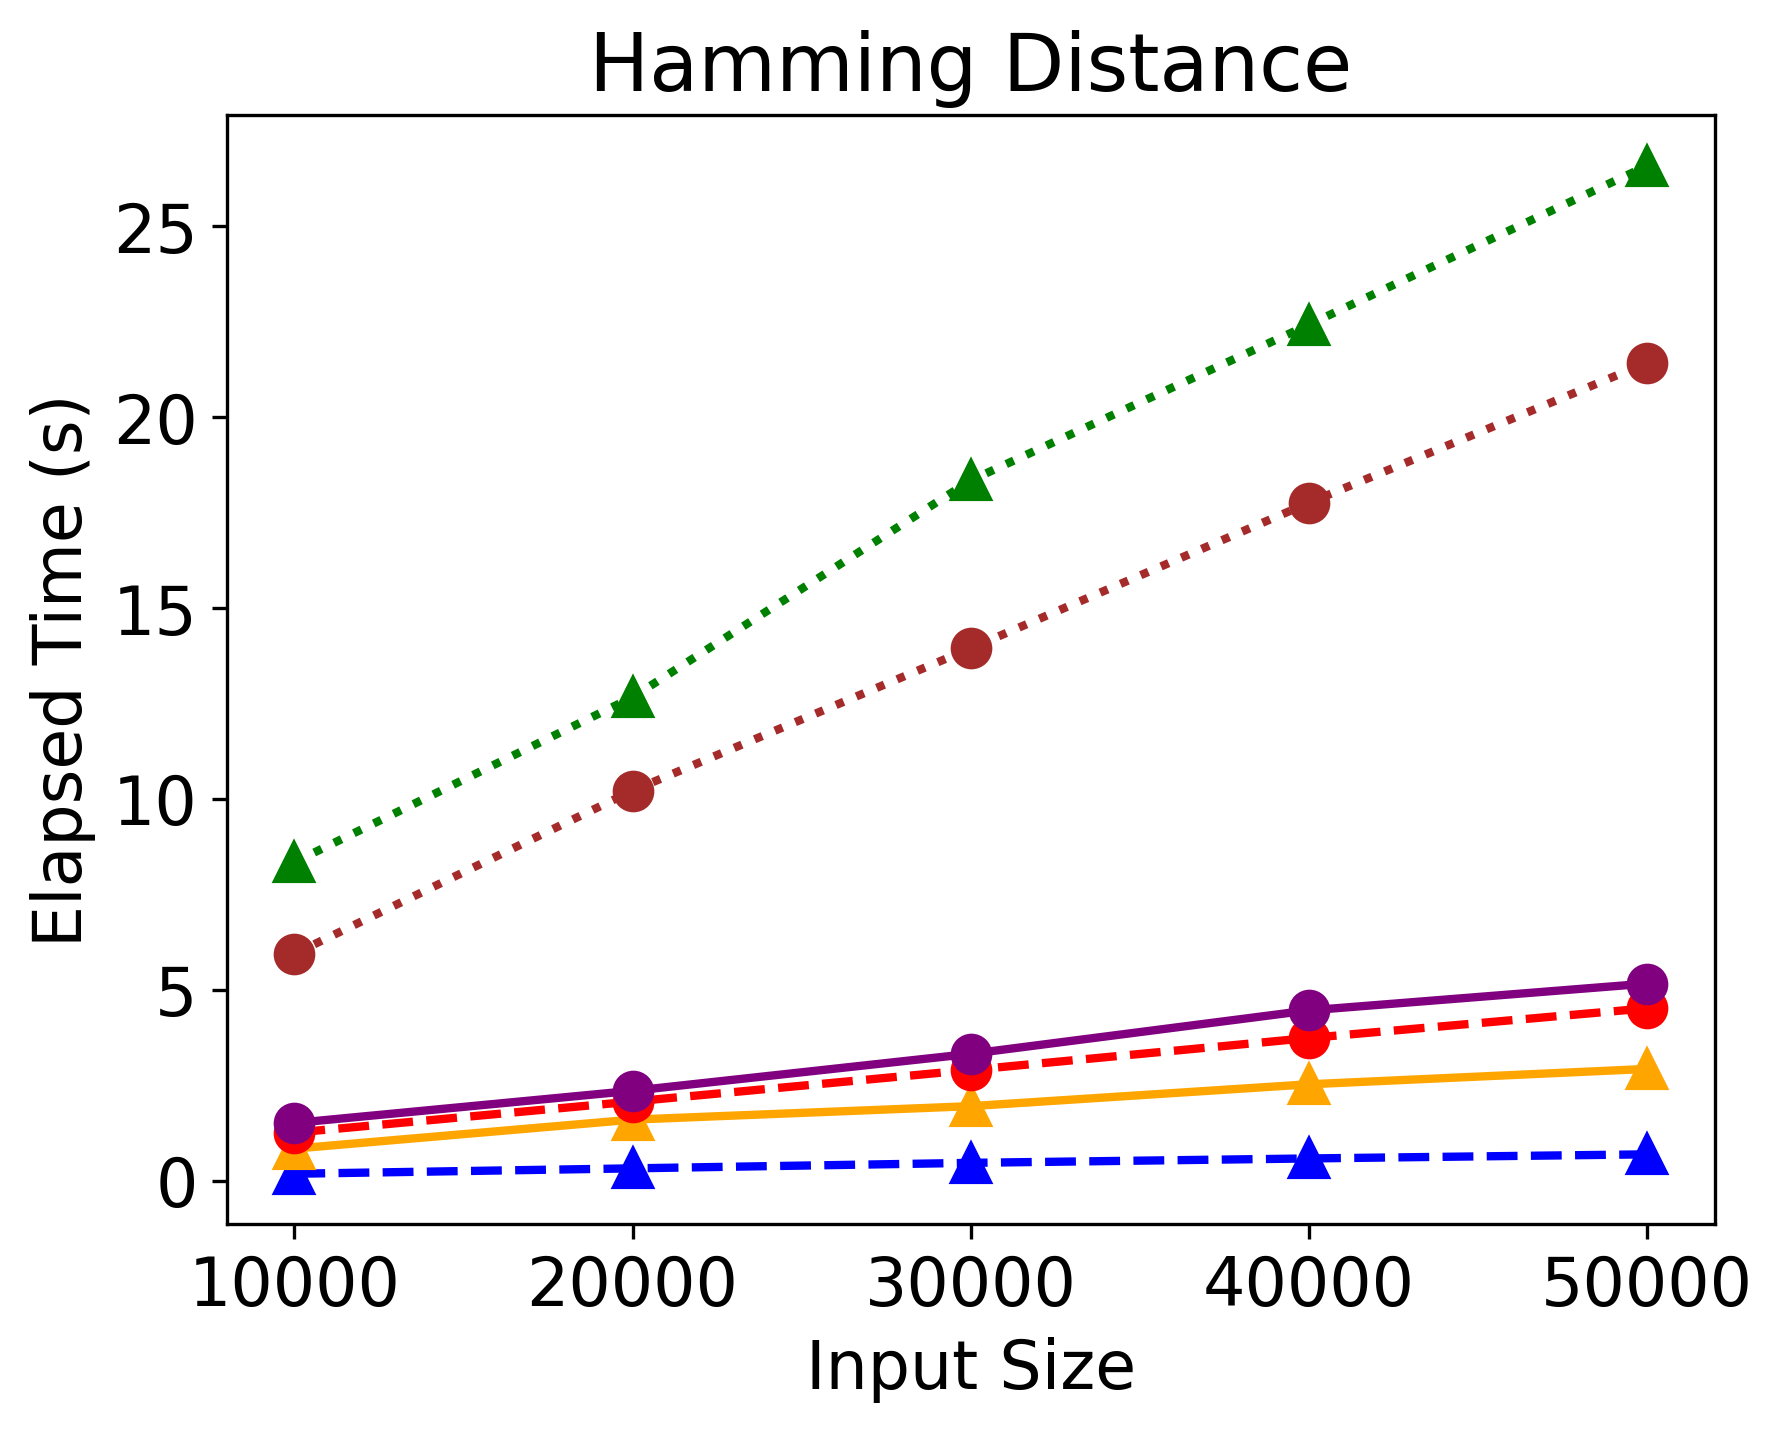
\includegraphics[width=.33\linewidth,align=t]{../figures/hamming.png}
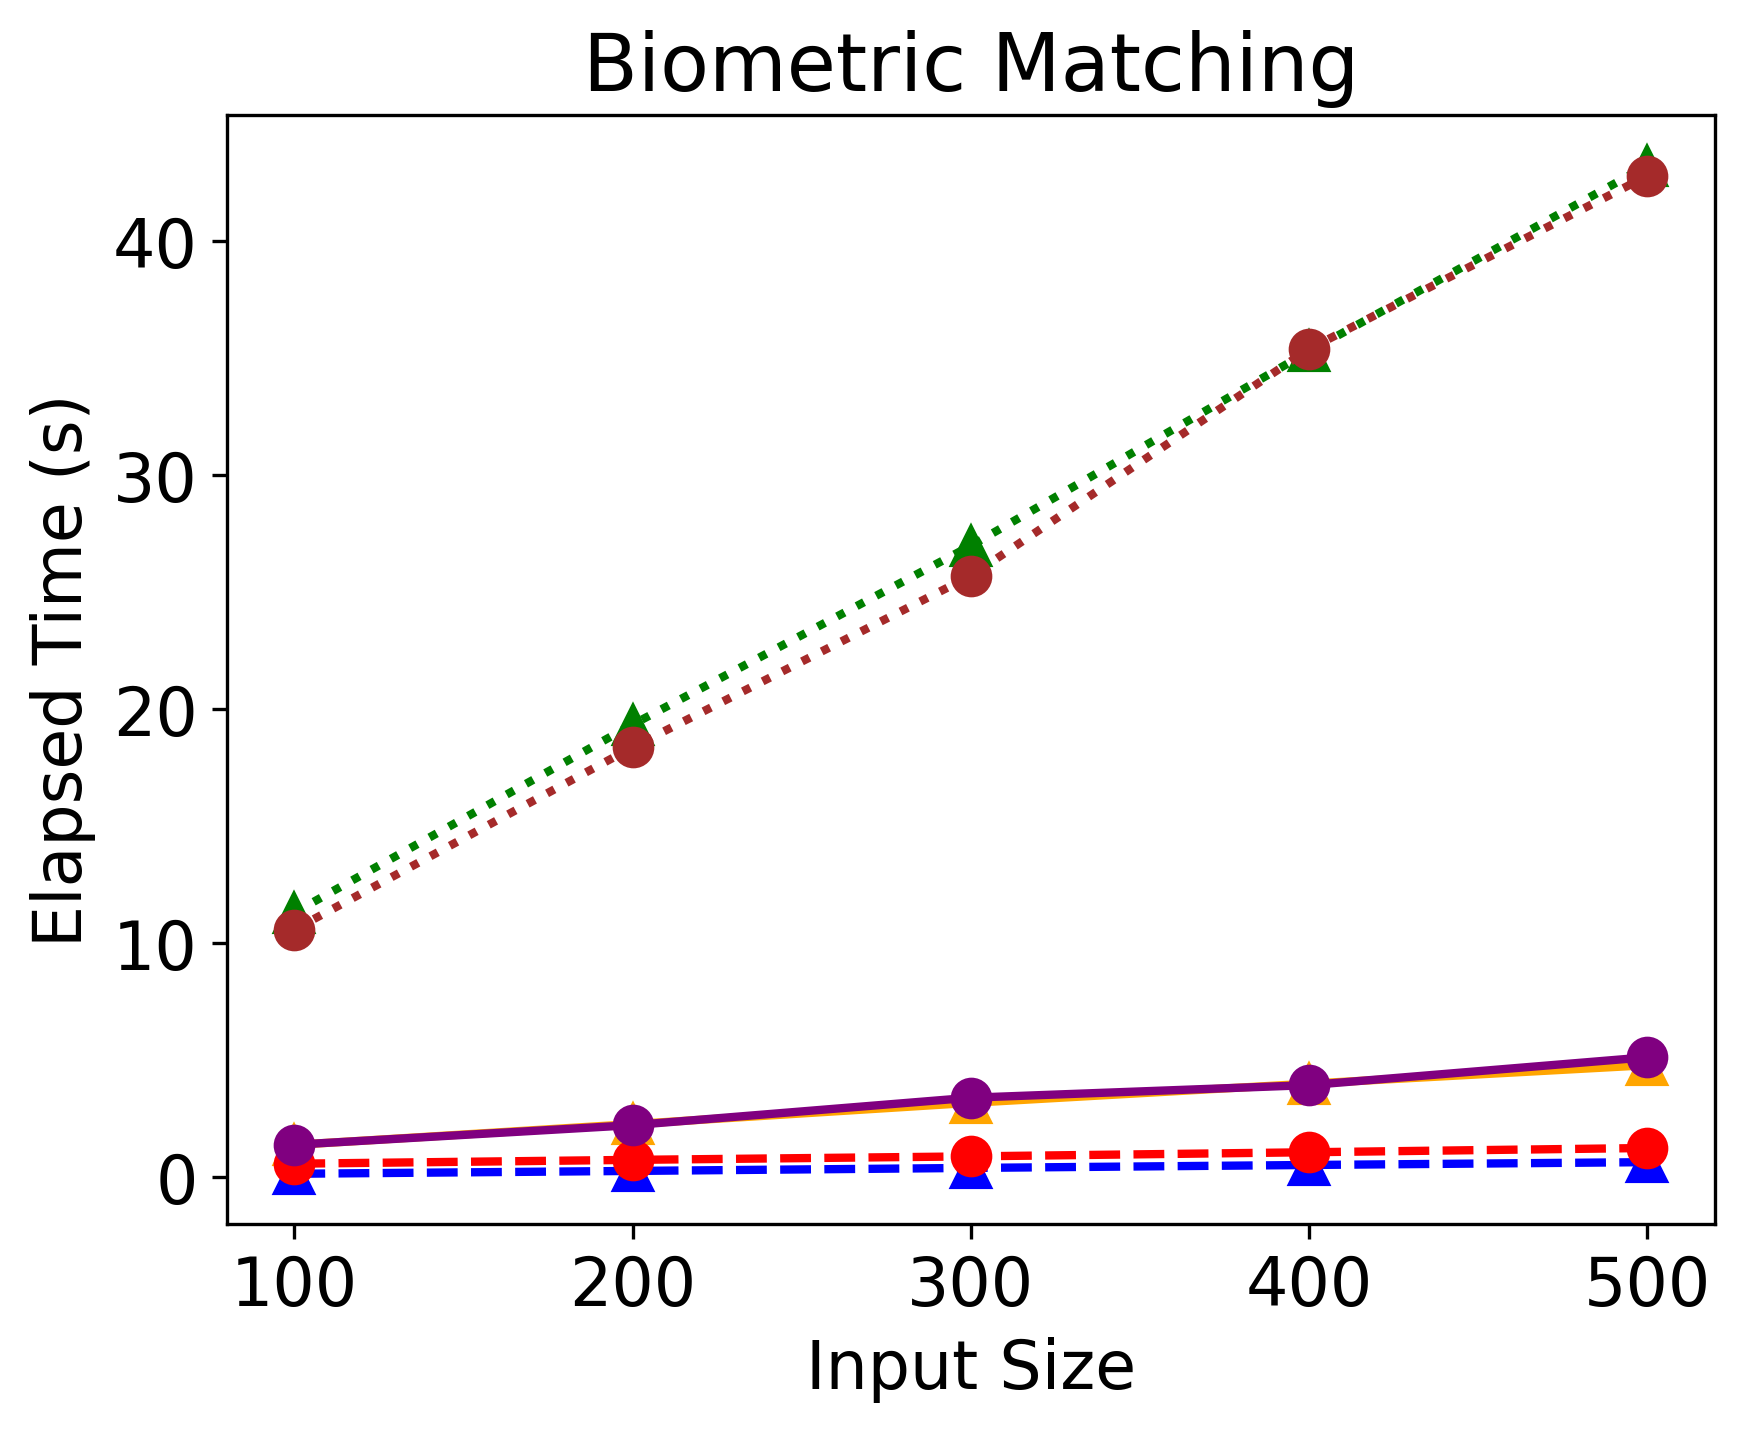
\includegraphics[width=.33\linewidth,align=t]{../figures/bio-matching.png}
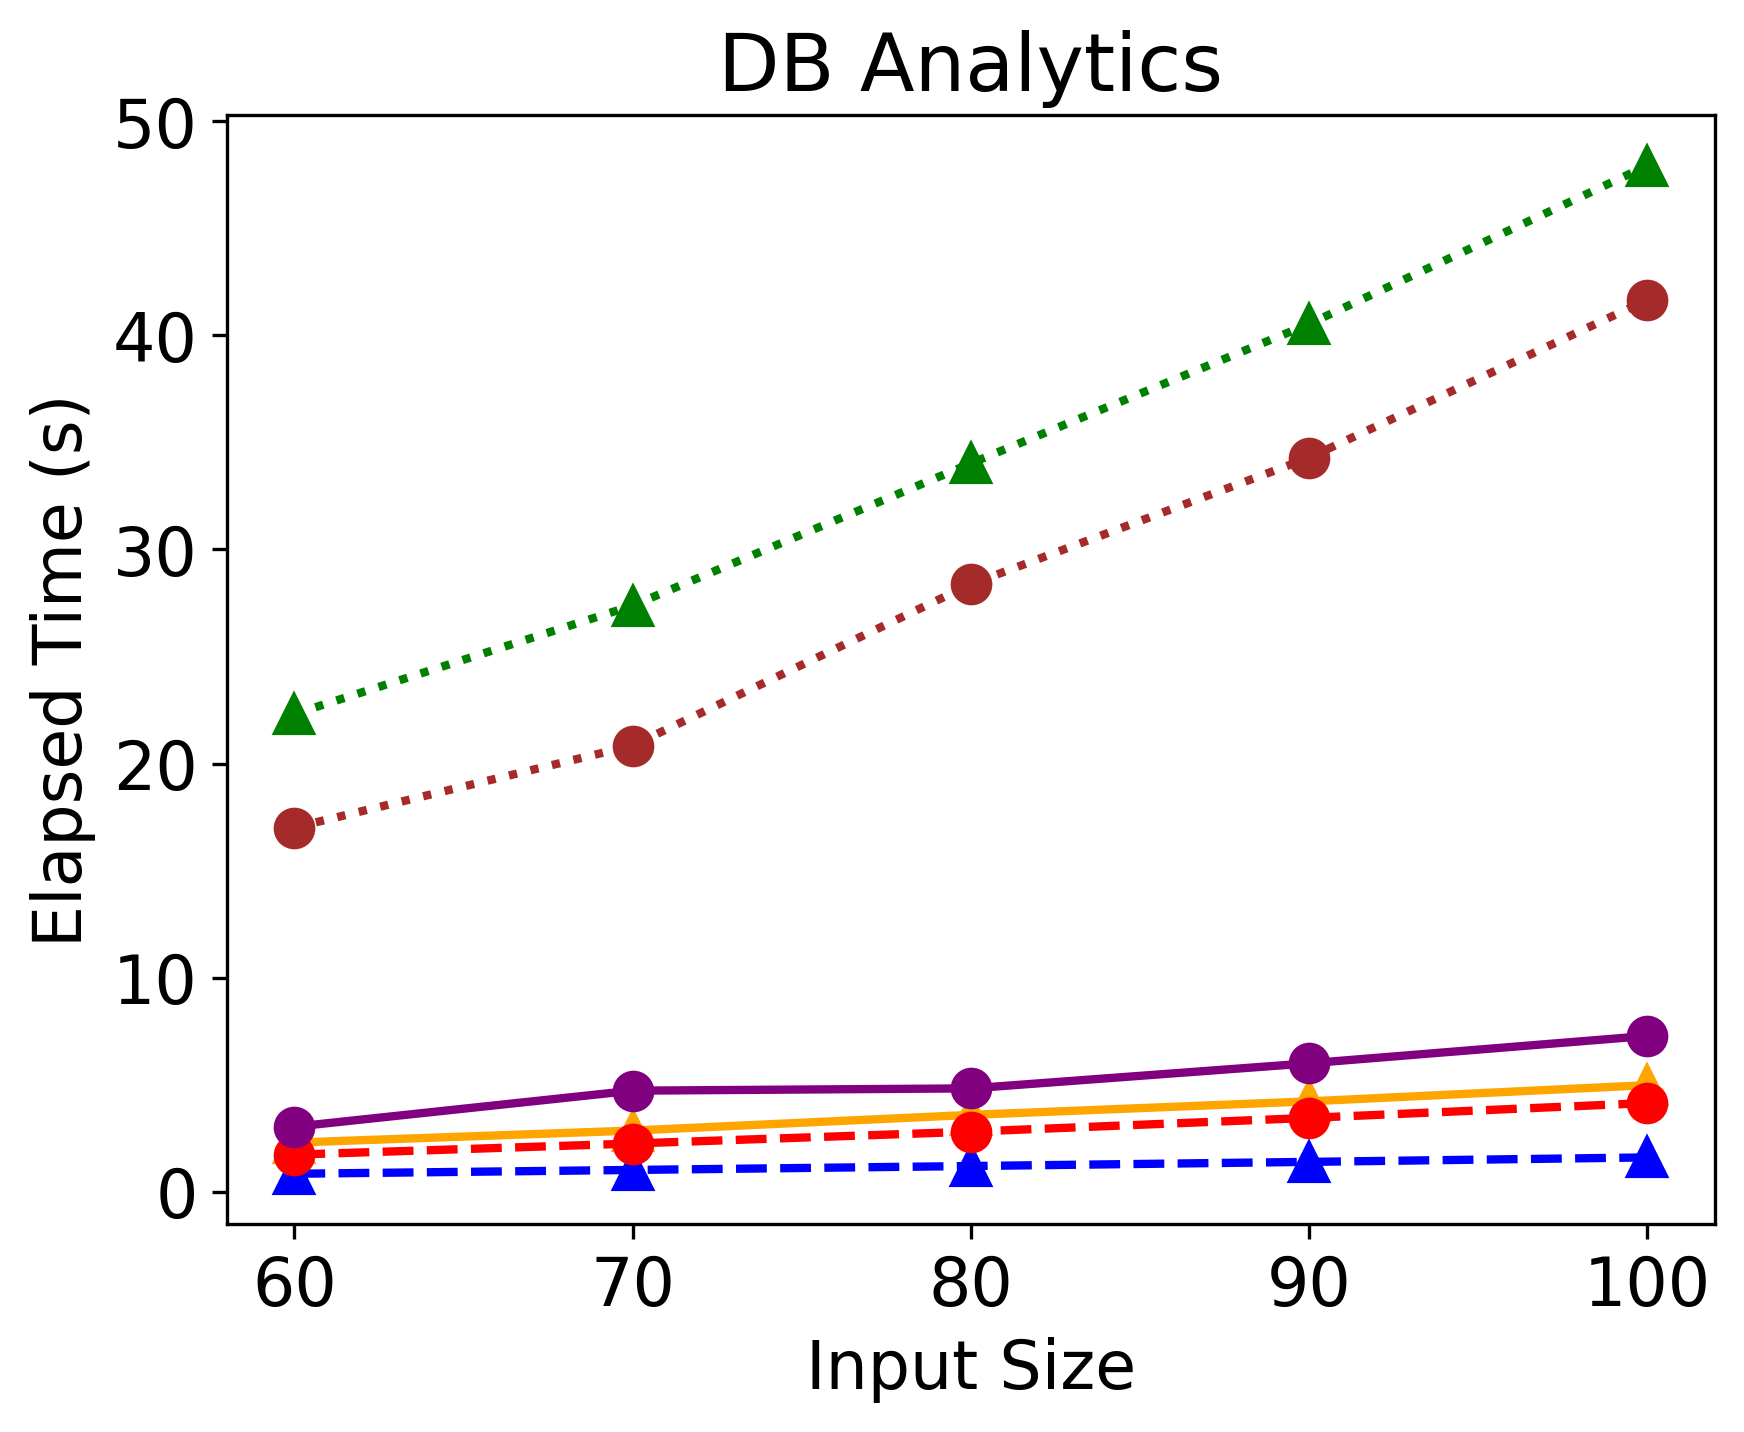
\includegraphics[width=.33\linewidth,align=t]{../figures/db-analytics.png}
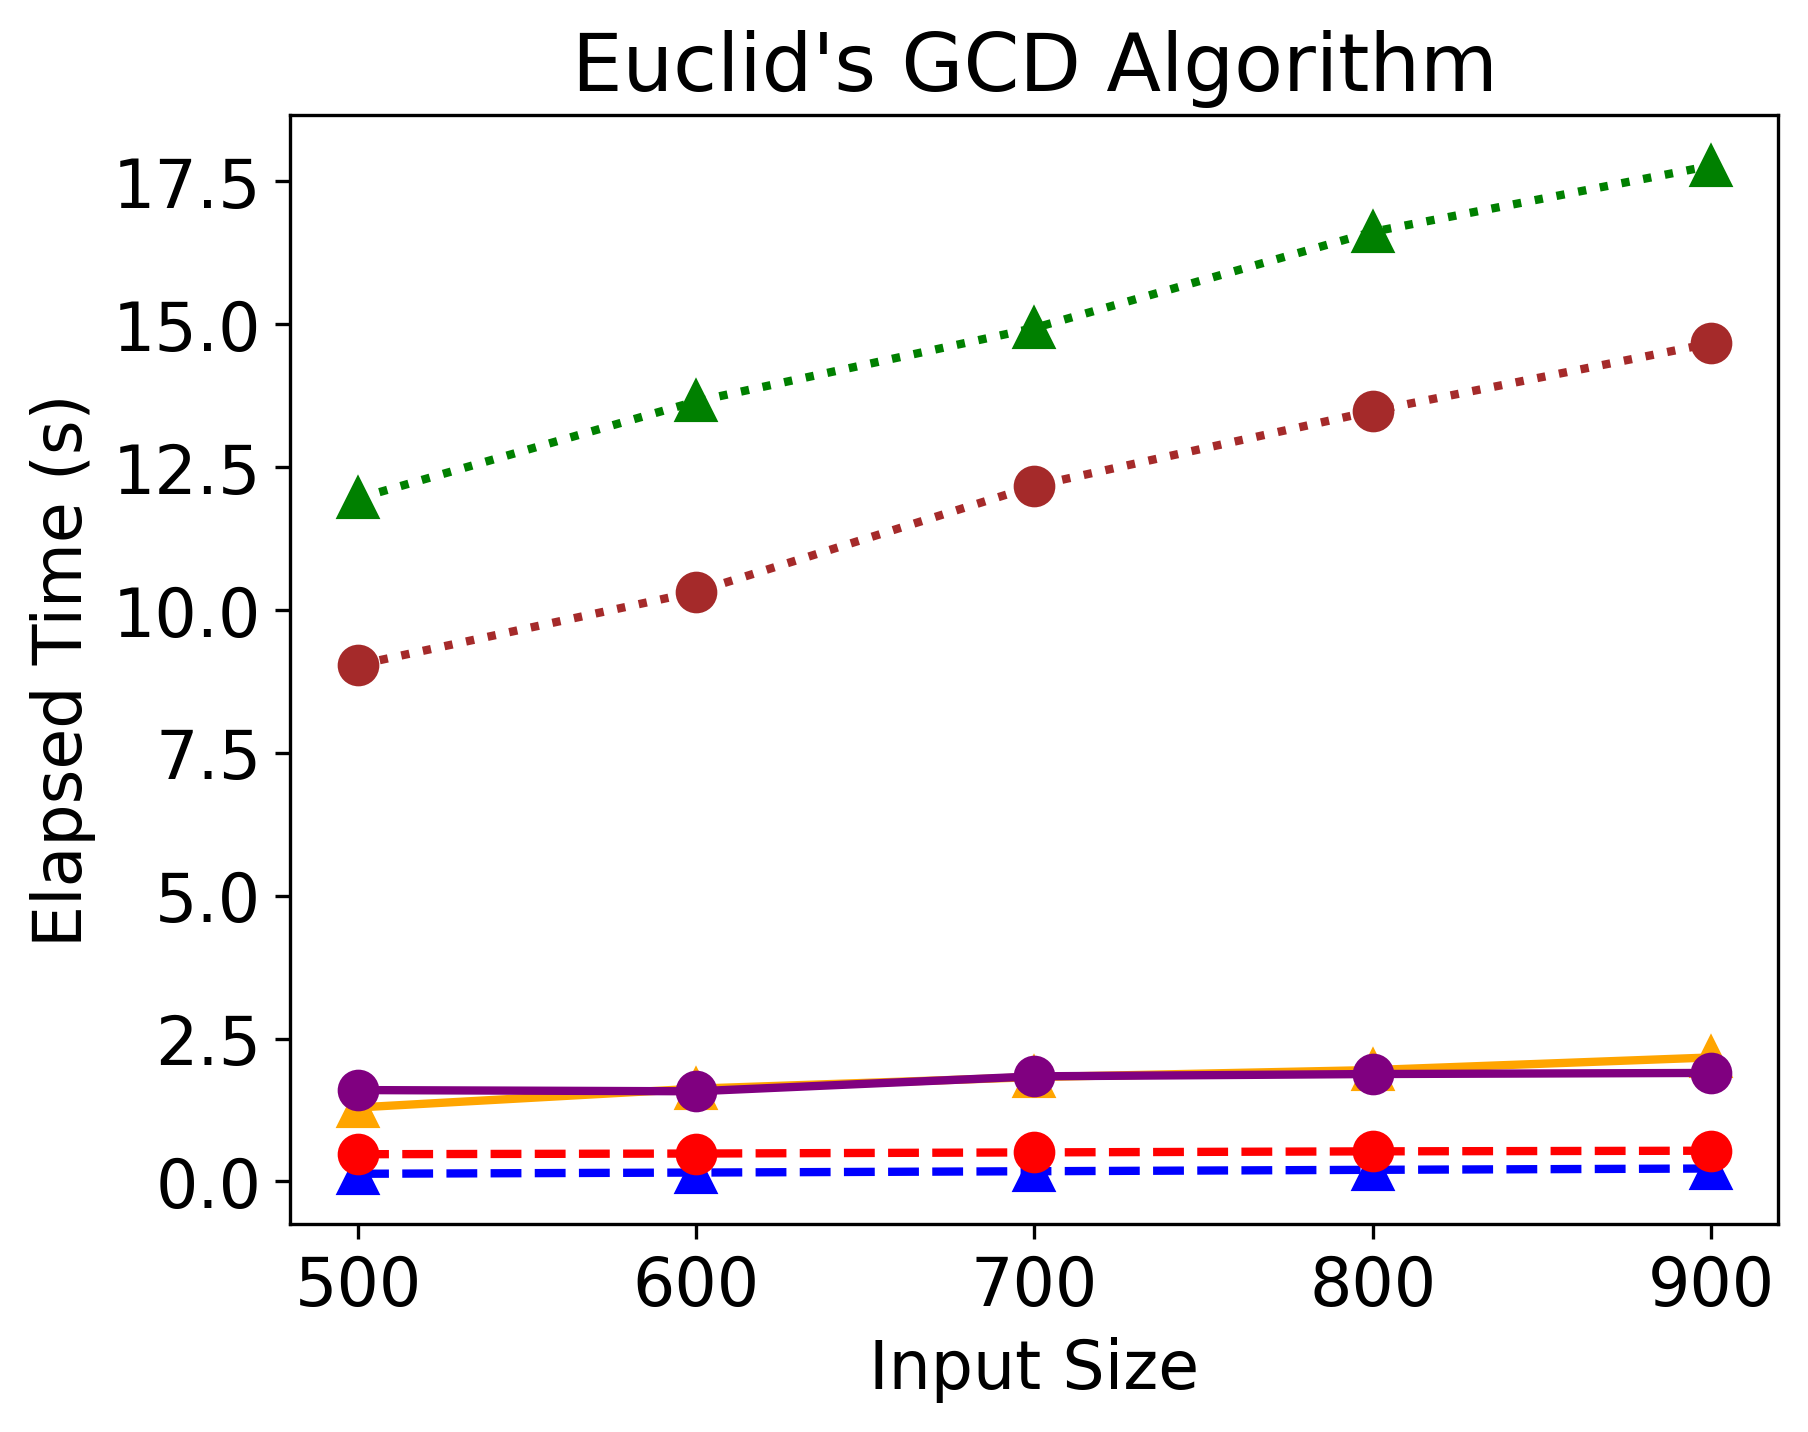
\includegraphics[width=.33\linewidth,align=t]{../figures/gcd-gc.png}
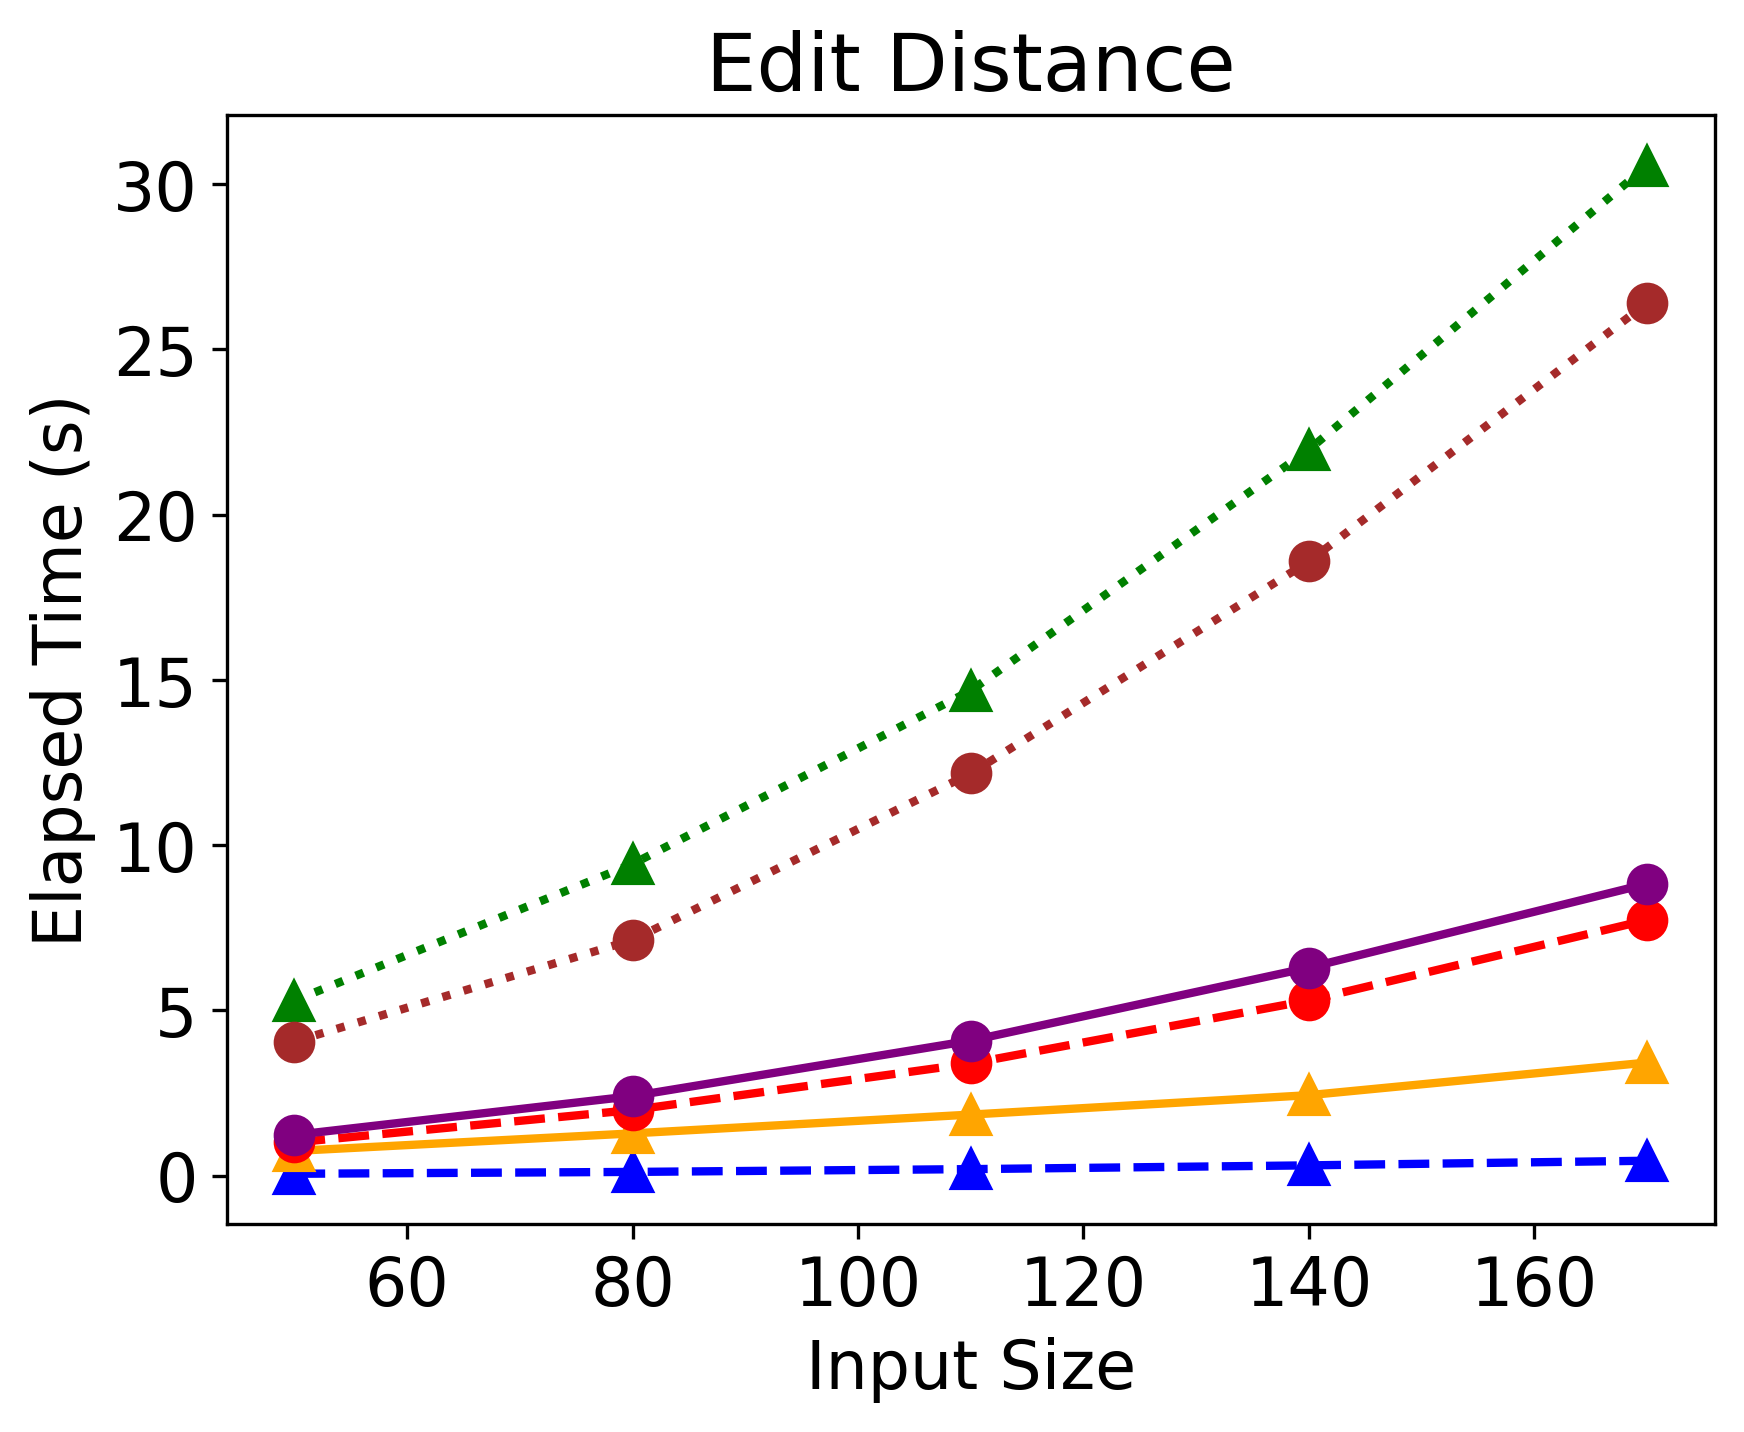
\includegraphics[width=.33\linewidth,align=t]{../figures/edit-distance.png}
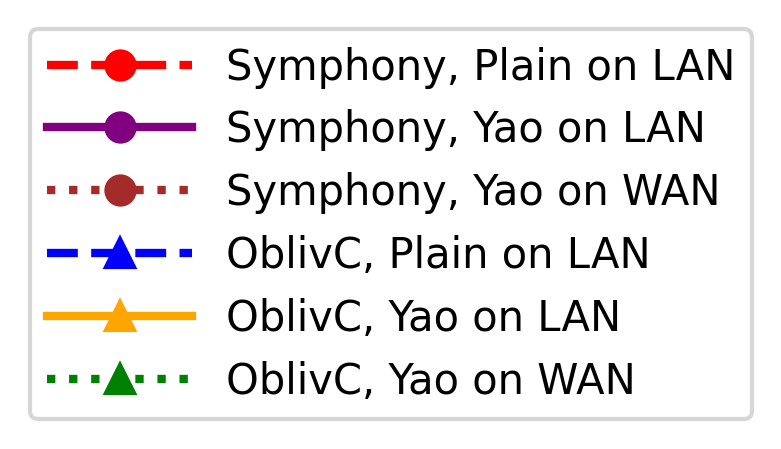
\includegraphics[width=.265\linewidth,align=t]{../figures/legend.png}
\caption{%
  End-to-end execution time (in seconds) of benchmarks, averaged over five samples.
  \textbf{LAN} is a simulated 1gbps connection with no delay. \textbf{WAN} is a simulated 100Mbps
  connection with a 50ms RTT latency. \textbf{Yao} and \textbf{Plain} protocols use EMP's \texttt{sh2pc}
  (semi-honest, two-party) and \texttt{plain} protocols respectively. \system{} uses EMP's Integer
  interface. OblivC uses EMP's Bit interface (compiling integer operations to circuits).
  Input sizes for all the benchmarks indicate the
  length of the list(s) provided as input, except for \texttt{gcd-gc} where the input size indicates
  the number of iterations of the GCD algorithm.
}\label{fig:mpc-impl-eval-etoe}
\end{figure*}

\paragraph{Runtime Performance}

Figure~\ref{fig:mpc-impl-eval-etoe} plots the end-to-end execution time of \system{}
and OblivC on the benchmarks. These results suggest that, as compared to OblivC,
\system imposes acceptable overhead. There are two primary sources for this overhead:

First, \system supports arbitrary numbers of parties while OblivC supports only two.
      This is significant because \system performs frequent runtime checks on the parties in scope.
      Since \system supports an arbitrary number of possible parties, we
      represent the parties in scope as a set (implemented by a balanced tree
      data structure).
      Thus checks on principals are implemented by set operations.
      OblivC also performs certain checks on parties but, since only two
      parties are supported, these are implemented as simple integer equality
      checks.

Second, our \system programs use linked lists and pattern matching while our
OblivC programs use arrays.  We believe that this is the dominant source of
overhead, and can be mitigated by rewriting \system programs to use arrays.

Comparing the LAN and WAN benchmarks confirms that the language overhead imposed by \system{} is dominated by
the time it takes to perform network communication during a WAN deployment of MPC. We believe \system{} is faster than OblivC in the WAN setting
due to its use of the EMP Integer interface, which uses the network
more efficiently than the Bit interface used by OblivC's callback
mechanism, and consequently the EMP backend for OblivC.

\paragraph{Generated Circuit Sizes}

\begin{table*}
  \centering
  \smaller
\begin{tabular}{ l l l l l l l l }
\hline \hline
& & \multicolumn{2}{c}{OblivC} & \multicolumn{2}{c}{\system{}} & \multicolumn{2}{c}{$\Delta$ (OblivC - \system{})} \\
\cmidrule(lr){3-4} \cmidrule(lr){5-6} \cmidrule(l){7-8}
Benchmark & Input Size & AND Gates & XOR Gates & AND Gates & XOR Gates & AND Gates & XOR Gates \\
\hline
Hamming Dist. & 10000 & 1249875  & 3159595  & 950000   & 2550000  & 299875  & 609595   \\
              & 20000 & 2499875  & 6319595  & 1900000  & 5100000  & 599875  & 1219595  \\
              & 30000 & 3749875  & 9479595  & 2850000  & 7650000  & 899875  & 1829595  \\
              & 40000 & 4999875  & 12639595 & 3800000  & 10200000 & 1199875 & 2439595  \\
              & 50000 & 6249875  & 15799595 & 4750000  & 12750000 & 1499875 & 3049595  \\
\hline
Bio. Matching & 100   & 2617868  & 6353496  & 2675500  & 8007000  & -57632  & -1653504 \\
              & 200   & 5235768  & 12706996 & 5351000  & 16014000 & -115232 & -3307004 \\
              & 300   & 7853668  & 19060496 & 8026500  & 24021000 & -172832 & -4960504 \\
              & 400   & 10471568 & 25413996 & 10702000 & 32028000 & -230432 & -6614004 \\
              & 500   & 13089468 & 31767496 & 13377500 & 40035000 & -288032 & -8267504 \\
\hline
DB Analytics  & 60    & 4609304  & 9569553  & 4732457  & 10425422 & -123153 & -855869  \\
              & 70    & 6246968  & 12970159 & 6413597  & 14128242 & -166629 & -1158083 \\
              & 80    & 8133020  & 16886701 & 8349937  & 18393262 & -216917 & -1506561 \\
              & 90    & 10268008 & 21320663 & 10541477 & 23220482 & -273469 & -1899819 \\
              & 100   & 12651370 & 26270229 & 12988217 & 28609902 & -336847 & -2339673 \\
\hline
GCD           & 500   & 2360091  & 6735821  & 2302192  & 6910016  & 57899   & -174195  \\
              & 600   & 2832991  & 8085621  & 2762592  & 8291916  & 70399   & -206295  \\
              & 700   & 3305891  & 9435421  & 3222992  & 9673816  & 82899   & -238395  \\
              & 800   & 3778791  & 10785221 & 3683392  & 11055716 & 95399   & -270495  \\
              & 900   & 4251691  & 12135021 & 4143792  & 12437616 & 107899  & -302595  \\
\hline
Edit Dist.    & 50    & 780882   & 1704539  & 637372   & 1779607  & 143510  & -75068   \\
              & 80    & 2003142  & 4378936  & 1631872  & 4556407  & 371270  & -177471  \\
              & 110   & 3790602  & 8291824  & 3085372  & 8614807  & 705230  & -322983  \\
              & 140   & 6143262  & 13443100 & 4997872  & 13954807 & 1145390 & -511707  \\
              & 170   & 9061122  & 19832759 & 7369372  & 20576407 & 1691750 & -743648  \\
\hline
\end{tabular}
\caption{%
  \textnormal{
  Gate counts (AND and XOR) of select benchmark programs. \textbf{Input Size} for Hamming Dist.,
  Bio. Matching, DB Analytics, and Edit Dist. is the length of the input lists. For GCD, it is
  the maximum number of GCD iterations. Gate counts were collected by modifying EMP to record
  AND or XOR gate execution. \system{} uses EMP's Integer interface where applicable,
  OblivC uses EMP's Bit interface (compiling integer operations to circuits).
  }
}
\label{tab:mpc-impl-eval-gates}
\end{table*}

As a second experiment, we instrumented the EMP backend to count the number of utilized AND and XOR gates.
Counting gates is primarily a sanity check that ensures \system is not
erroneously introducing large numbers of unneeded gates.
~\Cref{tab:mpc-impl-eval-gates} tabulates the number of
AND and XOR gates generated by \system{} and by OblivC.
The gate counts generated by \system{} and
OblivC are very similar, with differences caused by using the EMP
Integer interface vs OblivC compiling to the Bit interface (as
required by its callback mechanism. The optimizations
performed by EMP's circuit compiler and OblivC's circuit compiler are similar,
but not identical.

\paragraph{Experimental Conclusions}
Overall, our experiments indicate that the langauge design itself does not
impose significant overhead on either end-to-end execution time or generated
circuit sizes.
At the same time, \system{} is more expressive than frameworks like
OblivC (e.g., by allowing $N$ parties interleave many secure and cleartext computations)
and safer (e.g., by guaranteeing that the distributed deployment matches local
development). We leave a more sophisticated implementation which leverages
compilation, compiler optimizations, and mutable arrays, as future work. We
conjecture that such an implementation would be quite competitive with existing
state-of-the-art MPC languages.

\chapter{\obliv, A Language for Probabilistically Oblivious Computation}
\label{ch:obliv}

\mwh{Same point here as the last chapter: What's the high-level
  takeaway for a committee member that just wants to see the dots and
  assess the big picture, rather than see the detailed connections
  between the dots?}

An oblivious computation is one that is free of direct and indirect information leaks, e.g., due to observable differences
in timing and memory access patterns. In this chapter, we'll give a formal description of \obliv, a core language whose
type system enforces obliviousness. We show that \obliv satisfies~\nameref{thm:obliv-pmto}, a probabilistic variant of obliviousness.
We also show that \obliv's type system is expressive enough to typecheck an asymptotically optimal client-server ORAM implementation.

\section{Design}
\label{sec:obliv-design}

The formal language design consists of the syntax (\Cref{fig:obliv-syntax}), type system (\Cref{fig:obliv-types},
and a small-step, probabilistic operational semantics (\Cref{fig:obliv-sem}. The type system is sound, and designed to additionally
enforce that well-typed programs satisfy~\nameref{thm:obliv-pmto}. In other words, they are (probabilistically) oblivious.
The proof of~\nameref{thm:obliv-pmto} is complex and we elide the full details here. Interested readers can consult the full paper~\cite{}.

\FigureOblivSyntax{fig:obliv-syntax}{\obliv formal syntax.}

\subsection{Syntax}
\label{subsec:obliv-design-syntax}

Figure~\ref{fig:obliv-syntax} shows the syntax for \obliv. The term language is
expressions ⸨e⸩. The set of values ⸨v⸩ is comprised of (1) base values such as
variables ⸨x⸩ (included to enable a substitution-based semantics) and recursive function
definitions ⸨⦑fun⦒⸤y⸥(x{⦂}τ).e⸩ where the function body may refer to itself
using variable ⸨y⸩; and (2) connectives from the expression language ⸨e⸩ which
identify a subset of expressions which are also values, such as pairs ⸨⟨v,v⟩⸩
with type ⸨τ × τ⸩.

Expressions also include bit literals ⸨b⸤ℓ⸥⸩ (of type ⸨⦑bit⦒⸤ℓ⸥⸢⊥⸣⸩) which are
either ⸨⦑O⦒⸩ or ⸨⦑I⦒⸩ and annotated with their security label
⸨ℓ⸩.
%
A security label ⸨ℓ⸩ is either
⸨‹S›⸩ (secret) or ⸨‹P›⸩ (public). Values with the label ⸨‹S›⸩ are invisible to
the adversary. Bit types include this security label along with a probability
region ⸨ρ⸩. The expression ⸨⦑flip⦒⸢ρ⸣()⸩ produces a flip value, i.e.,
a uniformly random bit of type ⸨⦑flip⦒⸢ρ⸣⸩.
The annotation assigns the coin to region ⸨ρ⸩. Coin flips are semantically secret, and have
limited use; we can compute on one using ⸨⦑mux⦒⸩ or ⸨⦑xor⦒⸩, cast one to a
public bit via ⸨⦑cast⦒⸤‹P›⸥⸩, or cast to a secret bit via ⸨⦑cast⦒⸤‹S›⸥⸩. To
simplify the type system, casts only apply to values, however ⸨⦑cast⦒⸤ℓ⸥(e)⸩
could be used as shorthand for ⸨⦑let⦒␣x = e␣⦑in⦒␣⦑cast⦒⸤ℓ⸥(x)⸩.

The expression ⸨e₁ {¿} e₂ {◇} e₃⸩ unconditionally evaluates ⸨e₂⸩ and ⸨e₃⸩ and
returns their values as a pair in the given order if ⸨e₁⸩ evaluates to ⸨⦑I⦒⸩, or in the
opposite order if it evaluates to ⸨⦑O⦒⸩. This is very similar to the multiplexor
from \mpc, except that it returns a pair. The components of tuples
⸨e⸩ constructed as ⸨⟨e₁,e₂⟩⸩ can be accessed via ⸨⦑let⦒␣x₁,x₂=e␣⦑in⦒␣...⸩
\obliv also has normal let binding, function application, and means to manipulate
mutable reference cells.

\obliv captures the key elements that make implementing oblivious
algorithms possible, notably: random and secret bits, trace-oblivious
multiplexing, public revelation of secret random values, and general
computational support in tuples, conditionals and recursive functions.
Other features can be encoded in these, e.g., general numbers and
operators on them can be encoded as tuples of bits, and arrays can be
encoded as tuples of references (read/written using (nested) conditionals).
Our prototype interpreter implements these things directly.

\FigureOblivSemantics{fig:obliv-sem}{\obliv semantics.}

\subsection{Semantics}
\label{subsec:obliv-design-sem}

\Cref{fig:obliv-sem} presents a monadic, probabilistic small-step
semantics for \obliv programs. The top of the figure contains some new and
extended syntax. Values (and, by extension, expressions) are extended with
forms for bit values ⸨⦑bitv⦒⸤ℓ⸥(b)⸩, flip values ⸨⦑flipv⦒(b)⸩, and
reference locations ⸨⦑locv⦒(ι)⸩; these do not appear in source programs. Stores
⸨σ⸩ map locations to values. Stores are paired with expressions to form
\emph{configurations} ⸨ς⸩. A sequence of configurations arising during an
evaluation is collected in a \emph{trace} ⸨t⸩.  We define evaluation
contexts ⸨E⸩ (not shown) in the style of~\citet{felleisen1992revised} to enforce a
left-to-right, call-by-value evaluation strategy.

The semantics is defined using the standard “denotational” discrete probability monad
⸨𝒟⸩~\cite{10.1007/BFb0092872,Ramsey:2002:SLC:503272.503288}.

In the probability monad ⸨𝒟⸩, the ⸨‹return›⸩ operation constructs a point
distribution, and the ⸨‹bind›⸩ operation encodes the law of total probability,
{i.e.}, constructs a marginal distribution from a conditional one. We only use
proper distributions in the sense that the combined mass of all elements sums
to 1. We do not denote possibly non-terminating programs directly into the
monad, and therefore do not require the use of computable
distributions~\cite{huang-computable-distributions} or
sub-probability distributions~\cite{monniaux-ai-prob}—we use the monad only to denote distributions of
configurations which occur after a finite number of small-step transitions,
which is total.

The definition of ⸨‹step›⸩ describes how a single configuration advances in a
single probabilistic step, yielding a distribution of resulting configurations.
The definition uses Haskell-style ⸨‹do›⸩ notation as the usual notation for
⸨‹bind›⸩. Starting from the bottom, we can see that a value ⸨v⸩ advances to
itself (more on why, below) and evaluating a redex ⸨e⸩ within a context ⸨E⸩
steps the former and packages its result back with the latter, as usual. The
cases for let binding, pair deconstruction, and function application are
standard, using a substitution-based semantics. Likewise, rules for creating,
reading, and writing from references operate on the store ⸨σ⸩ as
usual.

Moving to the first case, we see that literals ⸨b⸤ℓ⸥⸩ evaluate in one
step to bit values. A ⸨⦑flip⦒⸢ρ⸣()⸩ expression evaluates to either
⸨⦑flipv⦒(⦑I⦒)⸩ or ⸨⦑flipv⦒(⦑O⦒)⸩ as determined by ⸨‹bit›⸩, which ⸨½⸩
probability for each outcome.
%
The ⸨⦑cast⦒⸤ℓ⸥⸩ case converts a flip to a similarly-labeled bit value.
%
The next few cases use the three-argument metafunction ⸨‹cond›(b,X,Y)⸩, which
returns ⸨X⸩ if ⸨b⸩ is ⸨⦑I⦒⸩, and ⸨Y⸩ otherwise.
%
The two ⸨⦑bitv⦒⸤𝓁⸥(b) ¿ v₂ ◇ v₃⸩ cases operate in a similar way: they return the
second two arguments of the multiplexor in order when the first
argument is ⸨⦑bitv⦒⸤ℓ⸥(⦑I⦒)⸩, and in reverse order when it is
⸨⦑bitv⦒⸤ℓ⸥(⦑O⦒)⸩. The security label of the result is the join of the labels of
all elements in involved. (This is not needed for flip values, since these are
always fixed to be secret.)
%
The case for ⸨⦑if⦒⸩ also uses ⸨‹cond›⸩ in the expected manner. The
case for ⸨⦑xor⦒⸩ permits xor-ing a bit with a flip, returning a
flip.

The bottom of the figure defines function ⸨‹nstep›(N,ς)⸩. It composes ⸨N⸩
invocations of ⸨‹step›⸩ starting at ⸨ς⸩ to produce a distribution of traces ⸨t⸩.

Both ⸨‹step›⸩ and ⸨‹nstep›⸩ are \emph{partial} in the usual way:
They are undefined (``stuck'') for nonsensical programs like
⸨⦑locv⦒(ι) (⦑bitv⦒⸤ℓ⸥(b))⸩ (treating a reference location as if it were
a function). The \obliv type system, explained next, rejects
such programs while also ensuring~\nameref{thm:obliv-pmto}.

\FigureOblivTypes{fig:obliv-types}{\obliv type system.}

\subsection{Type System}
\label{subsec:obliv-design-types}

Figure~\ref{fig:obliv-types} defines the type system for \obliv source programs
as rules for judgment ⸨Γ ⊢ e ⦂ τ ⨟ Γ'⸩, which states that under type
environment ⸨Γ⸩ expression ⸨e⸩ has type ⸨τ⸩, and yields residual type
environment ⸨Γ′⸩. We discuss typing configurations, including non-source
program values, in the next section. Type environments map variables to either
types ⸨τ⸩ or inaccessibility tags ⸨•⸩, which are used to enforce
affinity of flips. We discuss the three key features of the type
system---affinity, probability regions, and information flow
control---in turn.

\paragraph*{Affinity}
%
To enforce non-duplicability, when an affine variable is used by the
program, its type is removed from the residual
environment. Figure~\ref{fig:obliv-types} defines kinding metafunction ⸨𝒦⸩
that assigns a type either the kind universal ⸨⦑U⦒⸩ (freely duplicatable) or
affine ⸨⦑ A ⦒⸩ (non-duplicatable). Bits, functions, and references (but not
their contents, necessarily) are always universal,
and flips are always affine. A pair is considered affine if either of
its components is. Rule *⦗VarU⦘ in Figure~\ref{fig:obliv-types} types
universally-kinded variables; the output environment ⸨Γ⸩ is the same
as the input environment. Rule *⦗VarA⦘ types an affine variable by
marking it ⸨•⸩ in the output environment.

Rules *⦗Cast-S⦘ and *⦗Cast-P⦘ permit converting flips to bits
via the ⸨⦑cast⦒⸤‹S›⸥⸩ and ⸨⦑cast⦒⸤‹P›⸥⸩ coercions, respectively. The
first converts a ⸨⦑flip⦒⸢ρ⸣⸩ to a ⸨⦑bit⦒⸤‹S›⸥⸢ρ⸣⸩ and does \emph{not} make
its argument inaccessible (it returns the original ⸨Γ⸩) while the
second converts to a ⸨⦑bit⦒⸤‹P›⸥⸢⊥⸣⸩ and does make it inaccessible
(returning ⸨Γ'⸩). The type system is enforcing that any
random number is made adversary-visible at most once; secret copies
are allowed because they are never revealed.

References may contain affine values, but references themselves are
universal. Rather than track the affinity of aliased contents
specifically, the *⦗Read⦘ rule disallows reading out of a reference
cell whose contents are affine. Since the write operation returns the
\emph{old} contents of the cell, programs can see the existing
contents of any reference by first writing in a valid
replacement~\cite{Baker:1992:LLL:142137.142162}.

The *⦗Fun⦘ rule ensures that no affine variables in the defining
context are consumed within the body of the function, i.e., they are
not captured by its closure. We write ⸨Γ⊎[x↦‗, y↦‗ ]⸩ to split a
context into a part that binds ⸨x⸩ and ⸨y⸩ and a part ⸨Γ⸩ that binds the rest;
the ⸨Γ⸩ part is returned, dropping the ⸨x⸩ and ⸨y⸩
bindings. Both *⦗Let⦘ and *⦗Let-Tup⦘ similarly remove their bound
variables.

Finally, note that different variables could be made inaccessible in
different branches of a conditional, so *⦗If⦘ types each branch in the
same initial context, but then joins their the output contexts; if a
variable is made inaccessible by one branch, it will be inaccessible
in the joined environment. Contexts are joined pointwise, and the join of two
pointed types ⸨⇡•τ₁ ⊔ ⇡•τ₂⸩ is ⸨•⸩ when either ⸨⇡•τᵢ⸩ is ⸨•⸩, the same as
⸨⇡•τᵢ⸩ when both ⸨⇡•τᵢ⸩ are equal and not ⸨•⸩, and undefined otherwise.

\paragraph*{Information flow}
%
The type system aims to ensure that bits ⸨b⸤ℓ⸥⸩ whose security label
⸨ℓ⸩ is secret ⸨‹S›⸩ cannot be learned by an adversary. Bit types
⸨⦑bit⦒⸤ℓ⸥⸢ρ⸣⸩ include the security label ⸨ℓ⸩. The rules treat types
with different labels as distinct, preventing so-called \emph{explicit} flows. For
example, the *⦗Write⦘ rule prevents assigning a secret bit (of type
⸨⦑bit⦒⸤‹S›⸥⸢ρ⸣⸩) to a reference whose type is
⸨⦑ref⦒(⦑bit⦒⸤‹P›⸥⸢ρ⸣)⸩. Likewise, a function of type ⸨⦑bit⦒⸤‹P›⸥⸢ρ⸣ →
τ⸩ cannot be called with an argument of type ⸨⦑bit⦒⸤‹S›⸥⸢ρ⸣⸩, per the
*⦗App⦘ rule. In our implementation we relax *⦗App⦘ (but not *⦗Write⦘, due to
the invariance of reference types) to allow public bits
when secrets are expected; this is not done here just to keep things simpler.

The rules also aim to prevent \emph{implicit} information flows. A
typical static information flow type system~\cite{infoflow} would
require the type of the conditional's guard
to be less secret than the type of what it returns; e.g., the guard's
type could be ⸨⦑bit⦒⸤‹S›⸥⸢ρ⸣⸩ but only if the final type ⸨τ⸩ is secret
too. However, in \obliv we must be more restrictive: rule *⦗If⦘
requires the guard to be public since the
adversary-visible execution trace reveals which branch is taken, and
thus the truth of the guard. Branching on secrets must be done via
a multiplexor. Notice that rule *⦗Mux-Bit⦘ sets the label ⸨ℓ⸩ of the
each element of the returned pair to be the join of the labels on the
guard and the remaining components. As such, if the guard was secret,
then the returned results will be.  The *⦗Mux-Flip⦘ rule
always returns flips, which are invisible to the adversary, so the
guard can be secret or public.

\paragraph*{Probability regions.}
%
A probability region ⸨ρ⸩ appears on both ⸨⦑bit⦒⸩ and ⸨⦑flip⦒⸩
types. The region is a static name for a collection of flip values and
secret bit values that may be derived from them. A flip value is
associated with a region ⸨ρ⸩ when it is created, per rule *⦗Flip⦘. Rule
*⦗Cast-S⦘ ascribes the region ⸨ρ⸩ from the input ⸨⦑flip⦒⸢ρ⸣⸩ to the
output type ⸨⦑bit⦒⸤‹S›⸥⸢ρ⸣⸩, tracking the flip value(s) from which the
secret bit value was possibly derived. Per rule *⦗Bit⦘, bit literals
have probability region ⸨⊥⸩, as do public bits produced by
⸨⦑cast⦒⸤‹P›⸥⸩, per rule *⦗Cast-P⦘.

Regions form a join semi-lattice.
%
The type system maintains the invariant that flips at region ⸨ρ⸩ are
probabilistically independent of all secret bits in regions ⸨ρ′⸩ when
strictly ordered ⸨ρ′ ⊏ ρ⸩. Strict ordering is used because it is
«irreflexive» and «asymmetric». The semantic property of
interest—probabilistic independence—is likewise irreflexive (except
for point distributions), and asymmetry restricts future mux operations
between values in one direction only; we say more below.

Consider the *⦗Mux-Flip⦘ rule. If a secret
bit is typed at region ⸨ρ₁⸩ and a flip value at region ⸨ρ₂⸩, and ⸨ρ₁ ⫽⊏ ρ₂⸩,
then it may be that the values are correlated, and a ⸨⦑mux⦒⸩ involving the
values may produce flips that are non-uniform.
Both the *⦗Mux-Flip⦘ and *⦗Mux-Bit⦘ rules return outputs whose region is the join
of the regions of all inputs, indicating that the result of the ⸨⦑mux⦒⸩ is only
independent of values that were jointly independent of each of its components.

Because freshly generated random bits are always independent of each other, the
programmer is free to choose any regions when generating them via ⸨⦑flip⦒⸢ρ⸣()⸩
expressions. However, once chosen, the ordering establishes an invariant which
constrains the order in which mux operations can occur subsequently in the
program.
Let's look at how the type checker uses strict region ordering to accept and reject a safe and unsafe
multiplexor. The following code uses regions ⸨ρ₁ ⊏ ρ₂⸩.
\begin{center}
\begin{tabular}{cc}
\begin{minipage}{0.35\textwidth}
\begin{lstlisting}[escapeinside={([}{])}]
let sx,sy = (flip([$^{\rho_1}$])(),flip([$^{\rho_2}$])())
let sk,_ = castS(sx) ([⸨¿⸩]) sx ([⸨◇⸩]) sy
\end{lstlisting}
{\small (a) Incorrect example}
\end{minipage}
&
\begin{minipage}{0.45\textwidth}
\begin{lstlisting}[escapeinside={([}{])}]
 let sx = flip([$^{\rho_1}$])() in
 let sy,sz = castS(sx) ([⸨¿⸩]) flip([$^{\rho_2}$])() ([⸨◇⸩]) flip([$^{\rho_2}$])()
\end{lstlisting}
{\small (b) Correct example}
\end{minipage}
\end{tabular}
\end{center}
The type checker first ascribes types ⸨⦑flip⦒⸢{ρ₁}⸣⸩ and
⸨⦑flip⦒⸢{ρ₂}⸣⸩ to \code{sx} and \code{sy}, respectively, according to
rules *⦗Let-Tup⦘, *⦗Flip⦘, and *⦗Tup⦘. It uses *⦗Cast-S⦘ to give
\code{castS(sx)} type ⸨⦑bit⦒⸤‹S›⸥⸢{ρ₁}⸣⸩ and leaves \code{sx}
accessible so that *⦗VarA⦘ can be used to give it and \code{sy} types
⸨⦑flip⦒⸢{ρ₁}⸣⸩ and ⸨⦑flip⦒⸢{ρ₂}⸣⸩, respectively (then making them
inaccessible). Rule *⦗Mux-Flip⦘ will now fail because the independence
conditions do not hold. In particular, the region ⸨ρ₁⸩ of the
guard is not strictly less than the region ⸨ρ₁⸩ of the second
argument, i.e., ⸨ρ₁ ⫽⊏ ρ₁⸩.
%
The program labeled (b) above is well-typed.
Here, the bit in
the guard has region ⸨ρ₁⸩, the region of the two flips is ⸨ρ₂⸩ and ⸨ρ₁
⊏ ρ₂⸩ as required by *⦗Mux-Flip⦘. It is easy
to see that both \code{sy} and
\code{sz} are uniformly distributed and independent of \code{sx}.

Rule *⦗Xor-Flip⦘ permits xor'ing a secret with a flip, returning a
flip, as long as the secret's region and the flip's region are
well ordered, which preserves uniformity.

We might be tempted not to order regions but instead
maintain an invariant that flips and bits
in distinct regions are independent. This turns out to not work.
%
While at the outset a fresh flip value is independent of all other
values in the context of the program, the region ordering is needed to
ensure that multiplexor operations will only occur in ``one direction.''
{E.g.}, if two fresh flip values are created ⸨x = ⦑flip⦒⸢ρ₁⸣()⸩ and ⸨y
= ⦑flip⦒⸢ρ₂⸣⸩, it is true that ⸨x⸩ and ⸨y⸩ are mutually independent. Thus it would
seem reasonable that ⸨⦑cast⦒⸤S⸥(x) ¿ y ◇ …⸩ and
⸨⦑cast⦒⸤S⸥(y) ¿ x ◇ …⸩ should both be well typed. While they are
both safe in isolation, the combination is problematic. Consider the
results of each mux---they are both flip values, and they are both
valid to reveal using ⸨⦑cast⦒⸤P⸥⸩ individually. However, the resulting
values are correlated (revealing one tells you information about the
distribution of the other), which violates the uniformity guarantee of
all ⸨⦑cast⦒⸤P⸥⸩ results. By ordering the regions, we are essentially
promising to only allow ⦑mux⦒ operations like this in one direction
but not the other, and therefore uniformity is never violated for
revealed flip values. For example, by requiring ⸨ρ₁ ⊏ ρ₂⸩ we allow the
first multiplexor above but not the second.

\paragraph*{Type safety}

\obliv is type safe in the traditional sense, i.e., that a well-typed
program will not get stuck. However, our interest is in the stronger
property that type-safe \obliv programs do not reveal secret
information via inferences an adversary can draw from observing their
execution. We state and prove this stronger property in the next section.

\FigureOblivObs{fig:obliv-obs}{\obliv adversary observability.}

\subsection{Probabilistic Memory Trace Obliviousness}
\label{subsec:obliv-design-pmto}

The main metatheoretic result of this chapter is that \obliv's type
system ensures probabilistic memory trace obliviousness (PMTO). This
section defines the property, but does not go into details on the proof.

\Cref{fig:obliv-obs} presents a model ⸨‹obs›⸩ of the adversary's view of
a computation as a new class of values,
expressions and traces that ``hide'' sub-expressions
considered to be secret (written ⸨•⸩).  Secret bit expressions, secret bit values, and secret flip
values all map to ⸨•⸩. Compound values, expressions, stores, traces etc. call ⸨‹obs›⸩ in recursive
positions as expected.

Probabilistic memory trace obliviousness (PMTO), stated formally
below, holds when observationally equivalent configurations induce
distributions of traces that are themselves observationally equivalent
after $N$ steps, for any $N$.\footnote{Noninterference
  properties are often stated with a non-empty store.
  Our notion of expression equivalence is simpler, and supports
  low-equivalent expressions that pre-populate such a
  store, so there is no loss of generality.}
\begin{proposition}[PMTO]\label{thm:obliv-pmto}
  J⁅ If: ⸨e₁⸩ and ⸨e₂⸩ are closed source expressions, ⸨⊢ e₁ ⦂ τ⸩, ⸨⊢ e₂ ⦂ τ⸩ and ⸨‹obs›(e₁) = ‹obs›(e₂)⸩
  J⁃ Then: (1) ⸨‹nstep›(N,e₁)⸩ and ⸨‹nstep›(N,e₂)⸩ are defined
  J⁃ And: (2) ⸨⇡~*{‹obs›}(‹nstep›(N,e₁)) = ⇡~*{‹obs›}(‹nstep›(N,e₂))⸩.
  J⁆
\end{proposition}
\noindent
(1) ensures that information is not leaked due to lack of progress, {i.e.}, if
either program gets “stuck,” and that the main property (2) applies to all
related, well-typed source expressions ⸨e₁⸩ and ⸨e₂⸩.

\section{Implementation}
\label{sec:obliv-impl}

We have implemented an interpreter and type checker for \textsc{OblivML},  a language that extends \obliv in
several (straightforward) ways.
%
First, we add natural number literals and random values; these can be
  encoded in \obliv as fixed-width tuples of ⸨⦑bitv⦒⸩ and ⸨⦑flipv⦒⸩
  respectively. We write them annotated with a security level, e.g.,
  \code{2 S} or \code{2 P}, and write \code{rnd R ()} to generate a
  random number at region \code{R}. We write \code{natS} to be the
  type of a secret number in region ⸨⊥⸩; \code{natP} for the type of a
  public number; \code{R natS} for the type of a secret number in the
  region \code{R}.  We also write \code{R rnd} to be the
  type of a random natural number in the region \code{R}.
Second, we add arrays; in our code examples, we write
  \code{a[n]} and \code{a[n] <- e} to read and write array
  elements. An array of length $N$ can be encoded in \lang as
  an $N$-tuple of references, using nested conditional expressions to
  access the correct (public) index and swapping out affine
  contents, as must be done with references.
Finally, we add records, which are like tuples but permit field accessor
  notation, \code{r.x}; if \code{x} is affine, doing so only consumes the field \code{x}
rather than consuming all of \code{r}.

To demonstrate the expressiveness of \obliv, we used our interpreter to
program (and type check) a series of interesting oblivious
algorithms. We have implemented a modern \emph{non-recursive, tree-based ORAM} (NORAM), which
is a key component of state-of-the-art ORAM implementations~\cite{asiacrypt11,pathoram,circuitoram}.
To our knowledge, ours is the first implementation automatically verified to
be oblivious. Building on this NORAM, we also implemented a full \emph{recursive} ORAM.
Type checking it requires some advanced (but standard) language features we
have not implemented, including region polymorphism, recursive and variant
types, and existential quantification. Finally, we have implemented \emph{oblivious stacks}
(ostacks), a kind of oblivious data structure~\cite{ods} that builds on top of NORAM.
In doing so, we discovered that oblivious stacks are cryptographically secure, but merely
statistically secure~\cite{sweet-plas21}. They actually do leak information, but the security claim is the
amount of leakage is negligible. Our implementation and all the examples discussed can be
found online at \url{https://github.com/plum-umd/oblivml}.

\chapter{\lang, A Probabilistically Oblivious Language for Secure Multiparty Computation}
\label{ch:proposal}

\mwh{For the parts not yet done, here: Don't formalize these. Instead,
  describe the properties/ideas you imagine you will implement. This
  is research so you don't have to know the result. But you can have
  ideas for the direction, and ideas on the problems you'll have to
  solve. It's worth writing those down.}

Up to this point, we have seen two languages (\mpc and \obliv) which, individually, have all the language
features that we are interested in. \obliv is \textbf{Probabilistic} and \textbf{High Assurance} while \mpc
is designed for MPC and \textbf{Abstractly Sequential}. The purpose of \lang is to unify these two languages
into a single MPC language satisfying all three properties. In this chapter, we formally propose \lang and
provide sketch of how it could be designed and implemented. Along the way, we point out potential difficulties
and hypothesize about how to overcome them.

\section{Design}
\label{sec:proposal-design}

The formal language design for \lang consists of the syntax (\Cref{fig:lang-syntax}), type system,
a probabilistic sequential semantics, and a probabilistic distributed semantics.
The type system should be sound, and additionally it should enforce~\nameref{thm:lang-pmto}. We claim that~\nameref{thm:lang-pmto}
is the appropriate extension of \obliv's~\nameref{thm:obliv-pmto} to the MPC setting. The ``\%" should be read as ``modulo'' and refers
to the PMTO proerty being generalized to handle declassifications. The last theorem we expect \lang to satisfy is~\nameref{thm:lang-simulation}
which is the appropriate extension of \mpc's~\nameref{thm:mpc-simulation} to the probabilistic setting.

\FigureLangSyntax{fig:lang-syntax}{\lang formal syntax.}

\subsection{Syntax}
\label{subsec:proposal-design-syntax}

The proposed syntax of \lang is in~\Cref{fig:lang-syntax}. The syntax of \lang builds primarily
on that of \mpc (\Cref{fig:mpc-syntax}), with the addition of some features from \obliv (\Cref{fig:obliv-syntax}).
The syntax is not presented in ANF (as \mpc was) for clarity. In the future, we will likely transition
to ANF to simplify the metatheory.

Most of \lang's expressions are standard and work identically to \mpc and \obliv.
We have variables ⸨x⸩; integers ⸨i⸩; booleans ⸨b⸩; party sets ⸨p⸩;
binary operations ⸨e ⊙ e⸩;
conditionals ⸨⦑if⦒␣e␣⦑then⦒␣e␣⦑else⦒␣e⸩; multiplexors ⸨e ¿ e ◇ e⸩;
sum creation ⸨ιᵢ␣e⸩ and elimination ⸨⦑case⦒␣x␣❴y⍪e⸤1⸥❵␣❴y⍪e⸤2⸥❵⸩;
pair creation ⸨⟨e,e⟩⸩ and elimination ⸨πᵢ␣e⸩;
reference creation ⸨⦑ref⦒␣e⸩, dereference ⸨¡x⸩, and assignment ⸨x ≔ y⸩;
function creation ⸨λ⸤z⸥x⍪ e⸩ and application ⸨x␣y⸩;
local variable binding ⸨⦑let⦒␣x=e⸤1⸥␣⦑in⦒␣e⸤2⸥⸩;
par(allel) execution ⸨⦑par⦒[e]␣e⸩;
local read ⸨⦑read⦒␣μ⸩ and write ⸨⦑write⦒␣e⸩;
MPC share ⸨⦑share⦒[e→e]␣e⸩ and reveal ⸨⦑reveal⦒⸤b⸥[e]␣e⸩;
uniform distributions ⸨⦑unif⦒⸢ρ⸣␣μ⸩;
and observation of distributions ⸨⦑observe⦒␣e⸩.

Literals no longer have a label ⸨l⸩ attached to them. Instead, we use
the combination of the location annotation ⸨@m⸩ and protocol annotation
⸨ψ⸩ as the information flow label.
The multiplexor, ⸨e₁ ¿ e₂ ◇ e₃⸩, works as in \mpc evaluating to either
⸨v₂⸩ or ⸨v₃⸩. The \obliv multiplexor can be encoded as
⸨e₁ ¿ e₂ ◇ e₃ ⩴ e₁ ¿ ⟨e₂,e₃⟩ ◇ ⟨e₃,e₂⟩⸩. Pairs are eliminated using
projection ⸨πᵢ⸩ as in \mpc rather than with pattern matching ⸨⦑let⦒␣x,y = e␣⦑in⦒␣e⸩
as in \obliv. The local read operation ⸨⦑read⦒␣μ⸩ takes a base type ⸨μ⸩ which is
type we expect to read. The reveal expression ⸨⦑reveal⦒⸤b⸥[e]␣e⸩ takes a boolean
⸨b⸩ indicating if the revelation is expected to be benign (zero-leakage). When
⸨b = ⦑true⦒⸩, we can think of this as acting like ⸨⦑cast⦒⸤‹P›⸥⸩ in \obliv. We rename
the ⸨⦑flip⦒⸢ρ⸣()⸩ expression from \obliv to ⸨⦑unif⦒⸢ρ⸣␣μ⸩ because we may generate
uniform booleans or integers. Finally, the ⸨⦑observe⦒␣e⸩ expression acts like ⸨⦑cast⦒⸤‹S›⸥⸩
from \obliv taking a uniform value and ``observing'' the underlying sample.

Types ⸨τ⸩ have location annotations, just like the values in the sequential semantics of \mpc (\Cref{fig:mpc-seq-aux}).
The located types ⸨σ⸩ refer recursively to types ⸨τ⸩. ⸨⦑prins⦒⸩ is the type of principal sets. The mode annotation ⸨m⸩ on function types ⸨τ ᵐ→ τ⸩ is the static
analog of the mode captured by closures in \mpc. Finally, our base types ⸨μ⸩ are augmented with three annotations. The probability
annotation, ⸨φ⸩, indicates whether this type is uniform or not. ⸨⦑\faThumbsUp⦒⸩ indicates a uniform type (⸨⦑flip⦒⸩ in
\obliv) and ⸨⦑\faThumbsDown⦒⸩ indicates a non-uniform type (⸨⦑bit⦒⸩ in \obliv). The probability region annotation, ⸨ρ⸩,
serves the same purpose as the annotation on the ⸨⦑flip⦒⸩ and ⸨⦑bit⦒⸩ types in \obliv. The protocol annotation, ⸨ψ⸩,
serves the same purpose as the protocol annotation in \mpc. So, for example, the ⸨⦑flip⦒⸢ρ⸣⸩ type from \obliv can be
represented as ⸨⦑bool⦒⸢⦑\faThumbsUp⦒ ; ρ ; ⋅⸣⸩ in \lang. This also allows us to represent, for example, the type
of encrypted uniform distributions of type ⸨μ⸩ among parties ⸨m⸩: ⸨μ⸢⦑\faThumbsUp⦒ ; ρ ; ⦑enc⦒⋕m⸣⸩. We can
also encode types representable in \mpc. For example, ⸨⦑int⦒⸢⦑\faThumbsDown⦒ ; ⊥ ; ⦑enc⦒⋕m⸣⸩, the type of non-random
(⸨⊥⸩) integers encrypted among parties ⸨m⸩.

\subsection{Sequential Semantics}
\label{subsec:proposal-design-seq}

We expect the sequential semantics of \lang to be a standard combination of the sequential
semantics of \mpc (\Cref{fig:mpc-seq}) and \obliv (\Cref{fig:obliv-sem}). In particular, we
expect to be able to take the sequential semantics of \mpc suitably extended and lift them
to the probabilistic setting by defining a monadic semantics in the style of \obliv in which
each \mpc rule corresponds to a \lang rule that produces a point distribution (⸨‹return›⸩ in
the Giry monad). For example, here's two candidate rules for introducing pairs and performing
a zero-information revelation.

P⁅ Rː⦗Allyn-ST-Pair⦘
   R⁅{Aːrcl
      A⁅ v₁ ⧼=⧽ γ(x₁)↙⸤m⸥
      A⁃ v₂ ⧼=⧽ γ(x₂)↙⸤m⸥
      A⁆}
      -------------------------------------------
      γ ⊢⸤m⸥ δ,⟨x₁,x₂⟩ ↪ ‹return›(δ,⟨v₁,v₂⟩@m)
      R⁆
P⁃ Rː⦗Allyn-ST-Reveal-True⦘
   R⁅{Aː[b]rcl
      A⁅ p@m          ⧼=⧽ γ(x₁)↙⸤m⸥
      A⁃ q@m          ⧼=⧽ γ(x₂)↙⸤m⸥
      A⁃ i⸢⦑\faThumbsUp⦒ ; ⦑enc⦒⋕p⸣@p ⧼=⧽ γ(x₃)↙⸤p⸥
      A⁆}
   R⁃{Aː[b]rcl
      A⁅ q ⧼≠⧽ ∅
      A⁃ m ⧼=⧽ p ∪ q
      A⁆}
      -------------------------------------------
      γ ⊢⸤m⸥ δ,⦑reveal⦒⸤⦑true⦒⸥[x₁→x₂]␣x₃ ↪ ‹return›(δ,i⸢⦑\faThumbsDown⦒⸣@q)
   R⁆
P⁆

We expect most rules to follow this adaptation pattern. However, one design decision
that must be made is whether or not to constrain the mode when evaluating a uniform
expression, ⸨⦑unif⦒⸢ρ⸣␣μ⸩. The simplest design is to force the mode to be a singleton.
If we want multiple parties to agree on a uniform value, it must be explicitly sent (shared)
with those parties. Alternatively, we could allow ⸨⦑unif⦒⸢ρ⸣␣μ⸩ to be evaluated in an arbitrary
mode ⸨m⸩. However, this is more challenging to realize in a distributed implementation since the
entropy on all parties has to be identical throughout execution to ensure that the uniform values
they generate are also identical. The advantage of this approach is that it is (potentially) faster
since there is no communication needed among the parties.

As we will see, most of the complexity of \lang crops up in the design of the type system, and the
proof strategies required for~\nameref{thm:lang-pmto} and~\nameref{thm:lang-simulation}.

\subsection{Type System}
\label{subsec:proposal-design-types}

There are three questions which must be addressed to effectively
design \lang's type system. First, what should the information-flow
labels be? Second, how do we type-check code which uses party sets as values?
Third, how do we type-check code which uses probability regions as values?

The information-flow labels have to be determined before obliviousness
can be enforced. The traditional public and secret labels don't make
sense in the MPC setting. A clear notion of the information-flow
lattice and labels is necessary because it is the foundational
definition of trust. If this is wrong, then security
theorems like non-interference and obliviousness are meaningless.

What should the typing rule for parallel execution ⸨⦑par⦒[e₁]␣e₂⸩ be?
To determine how the mode should be modified, we need to know the value
of the party set ⸨p⸩ which results from evaluating ⸨e₁⸩. This is what
makes type-checking code which uses party sets as values difficult.

Although not as clearly necessary, we also anticipate that we will
need to type-check code which uses probability regions as values.
For example, expressions like ⸨⦑unif⦒⸢e⸣␣μ⸩ where ⸨e⸩ evaluates
to a probability region ⸨ρ⸩.

\paragraph*{Information Flow Labels}

The traditional information-flow lattice for confidentiality is
typically the simple lattice denoting privileged (secret) and
unprivileged (public) entities. In this lattice, public is
ordered lower than secret. This lattice works well for traditional
information flow research in which there is a conceptual untrusted
client and trusted server. However, in MPC we typically think of
the various parties who are jointly computing as each having their
own secrets which they want to keep private from each other. In
that sense, it makes sense for the information-flow lattice to
be the (dual) powerset lattice over the universe of parties. The
bottom of the lattice is the universe of all parties, analogous
to ``public.'' The top of the lattice is the empty set, analogous
to ``secret.''

If we ignore MPC for a moment, then we can see that the location
annotations on types and values serve as static and dynamic information
flow labels. When a value is introduced, the mode determines its location (label).
When a value is eliminated, the mode is checked against its location (label).
The location checks necessary for simulation are pulling ``double-duty'' as
information-flow checks.

However, we must decide how MPC and encrypted types should be integrated into
the information-flow lattice. Our first attempt at such a lattice was to ``stack''
two powerset lattices, one for cleartext values and one for encryted values. We
use the location annotation as the label for cleartext values, and we use the
encryption annotation ⸨⦑enc⦒⋕m⸩ as the label for encrypted values. We then
sum these two lattices by asserting that top in the cleartext lattice ⸨⊤⸢‹c›⸣⸩
(cleartext values with empty location) are ordered below the bottom of the
encryption lattice ⸨⊥⸢‹e›⸣⸩ (encrypted values among all parties in the universe).
This approach breaks down when considering the least upper bound of a cleartext
label ⸨p⸢‹c›⸣⸩ and an encrypted label ⸨q⸢‹e›⸣⸩ where ⸨q ⊂ p⸩. The least upper
bound of two such labels is ⸨p⸢‹e›⸣⸩ according to the candidate lattice. However,
this doesn't match our intuition. A cleartext value known to ⸨p = \{A,B,C\}⸩ cannot
be used in a context that expects a value encrypted amongst ⸨q = \{A,B\}⸩.

We are confident that the location and encryption tags can be used to derive an appropriate
information-flow label, but it is ongoing work to figure out what the labels should be. Doing
so is a pre-requisite for the design of our type system.

\paragraph*{Polymorphic Types (Party Sets and Probability Regions)}

The most expressive type system design which handles first-class party sets
and probability regions is a dependent type system. Types would be allowed to
depend fully on party sets and probability regions (but not other kinds of values).
The advantage of this approach is that it is maximally expressive, meaning that
many programs can be made to type-check. The disadvantages are that it significantly
increases the burden on the language designer and the programmer. The language designer
must deal with issues such as normalization of open (symbolic) terms. The programmer
is often responsible for proving to the type-checker that a term has the appropriate type.
For example, if a given term ⸨e₂⸩ must be in mode ⸨m'⸩ in order to type-check, then the
programmer must prove that ⸨m ⊓ p = m'⸩ where ⸨p⸩ is the value of ⸨e₂⸩ at runtime.

A more ergonomic approach is to instead use refinement types. This approach is very expressive,
while eliminating the burden on the language designer and the programmer. The language
designer can offload reasoning about refinements to an auxiliary judgement which defers to
a decidable logical theory. Likewise, the programmer does not receive any proof obligations from
the type-checker. This same approach was taken by Wysteria~\cite{todo},
where refinements are singletons sets, subsets, or equality. Since \lang's ⸨⦑par⦒⸩ expressions
check non-empty intersection, we will likely also need to intersection as a value form.

\paragraph*{Adapting Obliviousness}

The definition of obliviousness for \lang must be adapted from the~\nameref{thm:obliv-pmto} theorem
to account for declassifications. In \mpc and \lang, revealing the result of an MPC computation
(potentially) leaks information about the secret inputs. There is a rich history of literature
on information-flow type systems which capture various security properties in the presence of
declassification. \citet{sabelfeldsandsjcs07} provides a comprehensive overview of these properties.
Our proposed definition of obliviousness is sketched in~\Cref{thm:lang-pmto}. Premise (1) says that
the closed programs ⸨e₁⸩ and ⸨e₂⸩ must be well-typed. Premise (2) says that ⸨e₁⸩ and ⸨e₂⸩ must be
indistinguishable to ⸨l⸩-observers. Premise (3) says that ⸨e₁⸩ and ⸨e₂⸩ both terminate, producing trace
distributions ⸨⇡~*{t₁}⸩ and ⸨⇡~*{t₂}⸩. Premise (4) says that the distribution of declassifications
in ⸨⇡~*{t₁}⸩ must be equivalent to the distribution of declassifications in ⸨⇡~*{t₂}⸩. If all of
these hold, then we may conclude that the trace distributions are indistinguishable to ⸨l⸩-observers.

\nameref{thm:lang-pmto} does not attempt to limit \emph{what} information may be released through a declassification.
Instead, it attempts to limit \emph{when} information may be released. In particular, it enforces that information may
only be released at declassifications (i.e. ⸨⦑reveal⦒⸤⦑false⦒⸥⸩). The ⸨ℛ⸩ metafunction achieves this by restricting
its view of the trace to only those configurations that contain a ⸨⦑reveal⦒⸤⦑false⦒⸥⸩ reducible expression. This means
that any reduction which is not a declassification will be ignored by ⸨ℛ⸩. If information is released somewhere else,
then premise (4) can still be satisfied, but the conclusion does not hold. We believe that this security theorem is
similar to Gradual Release~\cite{todo}. We believe that the primary difference between the two is that the presentation
of Gradual Release is epistemic, dealing with information release and attacker knowledge, whereas~\nameref{thm:lang-pmto}
is more syntactic, dealing with observable differences between pairs of traces.

The SCVM language~\cite{todo} proves a similar property, called ⸨Γ-simulatabilty⸩. This property is very similar to MTO\%
(non-probabilistic \nameref{thm:lang-pmto}), and to Gradual Release. The primary novelty in \lang is the generalization to
arbitrary parties (SCVM only supports two), and the generalization to the probabilistic setting.

\begin{theorem}[PMTO\%]\label{thm:lang-pmto}
  J⁅
  J⁃ If:  (1) ⸨e₁ : τ⸩, ⸨e₂ : τ⸩
  J⁃ And: (2) ⸨e₁ ≈⸤l⸥ e₂⸩
  J⁃ And: (3) ⸨e₁ ⇓ ⇡~*{t₁}⸩, ⸨e₂ ⇓ ⇡~*{t₂}⸩
  J⁃ And: (4) ⸨⇡~*ℛ⸤l⸥(⇡~*{t₁}) ≈ ⇡~*ℛ⸤l⸥(⇡~*{t₂})⸩
  J⁃ Then: ⸨⇡~*{t₁} ≈⸤l⸥ ⇡~*{t₂}⸩.
  J⁆
\end{theorem}

\subsection{Distributed Semantics}
\label{subsec:proposal-design-dist}

We expect the distributed semantics of \lang to be a straight-forward combination of the
distributed semantics of \mpc and \obliv. Since none of the expression forms added to
\lang require synchronization, we anticipate that these will be handled by \lang's version
of the *⦗DS-Step⦘ rule in~\Cref{fig:mpc-dist}. A \lang distributed configuration, ⸨ ⇡~*C ⸩,
will be a finite map from parties to \emph{distributions} of local configurations ⸨⇡.ς⸩.
We need not lift the distribution over the entire finite map, since there are no expressions
which are both probabilistic and synchronizing.

Here's an candidate adaptation of the *⦗DS-Step⦘ rule, according to the description above. As
a notational convenience, we notate distributions of local configurations as ⸨⇡^ς⸩.

P⁅ Rː⦗Allyn-DS-Step⦘
   R⁅ ⇡^ς —→⸤A⸥ ⇡^{ς'}
      ----------------
      ❴A ↦ ⇡^ς ❵ ⊎ ⇡~*C ↝ ❴A ↦ ⇡^{ς′} ❵ ⊎ ⇡~*C
   R⁆
P⁆

The local step relation, ⸨⇡^ς —→⸤A⸥ ⇡^ς⸩, is adapted in the same way as described
in~\Cref{para:mpc-design-dist-sem-nonsync}, and then the relation is lifted monadically.

We give a sketch of~\Cref{thm:lang-simulation} below, but the notation is intended to be evocative rather
than precise. We denote distributions using~⸨⇡~*{}⸩. Generally, we expect to have to lift most definitions from~\Cref{subsec:mpc-design-sim}
to a probabilistic variant. What does it mean for a distribution of configurations to be terminal? What is the definition of slicing, ⸨‗↯⸩,
over distributions of configurations? Does the natural lifting relate sequential and distribution configurations appropriately? These
are all questions we will investigate.

\begin{theorem}[Simulation (\lang)]\label{thm:lang-simulation}
    If ⸨ς ⇡~*{—→}⋆ ⇡~*{ς'}⸩ then ⸨⇡~*{ς'}⸩ is a terminal configuration and ⸨⇡~*C = ⇡~*{ς'}↯⸩ ⸨⟺⸩ ⸨ς↯ ⇡~*{↝}⋆ ⇡~*C ⸩ and ⸨ ⇡~*C ⸩ is a terminal configuration.
\end{theorem}

If we phrase the sequential semantics as a \emph{deterministic} semantics over \emph{distributions} of configurations
(rather than a \emph{probabilistic} semantics over \emph{individual} configurations) we may be able to recover much
of the proof strategy used in the proof of~\nameref{thm:mpc-simulation}. Since the distributions in the distributed
semantics are over local configurations, we anticipate that the semantics will still satisfy confluence up to equivalence
of distributions. Since the sequential semantics will still be deterministic (over distributions), we anticipate that the
proof of~\nameref{thm:lang-simulation} will also be easily adapted. The bulk of the work, then, will go to proving that
\lang satisfies Forward Simulation (appropriately adapted to distributions).

\section{Implementation}
\label{sec:proposal-impl}

Our implementation of \lang will build on the existing Haskell interpreter for \mpc, \system, described in~\Cref{sec:mpc-impl}.
The interpreter will need to be extended with support for a cryptographically secure PRNG. This will serve as a secure foundations for
generating uniform, random distributions which are suitable for use in cryptographic protocols. One possibility is to link the interpreter
against OpenSSL and use AES in CTR mode.

Perhaps the biggest implementation effort will be adding a sufficiently expressive type checker to the interpreter. As discussed
in~\Cref{subsec:proposal-design-types}, the type system will require polymorphism over probability regions and party sets. To
type check interesting programs, we will also need to support constraints over regions and party sets. To implement such a type system
will require linking against an SMT solver like Z3~\cite{} to check that constraints are satisfiable. All that being said, we have
implemented a type checker for \obliv as part of the \textsc{OblivML} interpreter so we anticipate that consulting this code
will make the implementation effort much easier.

As discussed in~\Cref{sec:mpc-impl}, the \system interpreter already has an extensive standard library, test suite, and benchmark
suite. We will evaluate how much of this existing \system code can be made to typecheck (i.e. by adding type annotations where necessary).
However, none of this existing code uses randomness. So, we anticipate that this will primarily evaluate the expressiveness of our
typing rule for party set polymorphism and associated constraints. To evaluate the expressiveness of code which uses randomness,
we'll implement a new set of benchmark programs. Our hope is to implement and type check One-Time Pad, Circuit ORAM,
Binary Search (on top of Circuit ORAM), and an optimized QuickSort using permutation~\cite{hamada}. All four of these programs
will rely on the type system to ensure that certain revelations leak zero information. The inclusion of One-Time
Pad and optimized QuickSort will provide evidence that our type system generalizes to programs beyond ORAM.

We will evaluate the efficiency of \lang using a methodology identical to the one described in \Cref{sec:mpc-impl} on the
benchmark programs described above (OTP, Circuit ORAM, Binary Search, and optimized QuickSort). We will also repeat the MPC
benchmarks to see how much performance improvement we achieve through static typing. We expect at least a modest improvement,
since we can omit all runtime checks for well-typed programs.

\chapter{Open Problems}
We briefly discuss some important open problems which affect the design of languages for
MPC and obliviousness. These are not addressed by \lang and we feel that they are promising
areas for future research.

\paragraph{Resource Awareness}
MPC programs are expensive. Small changes, such as using logical operators in place of multiplexors, can have dramatic
affects on execution time. The factors which affect performance include the circuit size, the amount of communication,
and the network's performance characteristics. For example in GMW, an AND gate requires a round of communication and the 1-4 OT requires an encryption scheme.
Programmers who are not experts in MPC will require information about the cost of the programs they are writing. There may
be opportunities to integrate resource-based reasoning into the language itself. Languages like Resource-Aware ML~\cite{10.1007/978-3-642-31424-7_64}
might provide a good starting place.

\paragraph{\lang Compiler}
Evaluating a sophisticated compiler for \lang against other MPC frameworks such as Obliv-C and ABY is left to future work. We conjecture
that such an implementation would be competitive with state-of-the-art MPC languages, while also providing strong safety and security
guarantees.

\paragraph{Oblivious Data Structures}
Our prior work has shown that Oblivious Data Structures (ODS's)~\cite{ods}, do not satisfy~\nameref{thm:obliv-pmto}.
Even though ODS's are safe due to negligible overflow probability, we are unable to verify that fact in \lang. We would like to find some
way to support ODS's within the language while retaining the security guarantees provided by the type system.

\paragraph{Other Security Policies}
PMTO\% is perhaps the most obvious security policy one could prove about MPC programs which admit ORAM. However, it is not the only property
one could prove. There is a rich literature of different declassification policies, as well as weaker variants of (P)MTO like Differential
MTO~\cite{10.5555/3310435.3310585} and manual computational proofs of security with explicit complexity-theoretic reductions~\cite{easycrypt}.

\paragraph{Usability of Abstractly Sequential Languages}
We claim in this proposal that abstractly sequential languages are a good choice for MPC. We justify that claim by arguing that
programmers need not think about the distributed deployment of their program. Furthermore, the type safety theorem for the sequential
semantics implies safety of the distributed semantics. However, a more empirical approach to the question of usability is warranted.
A user study comparing two languages, one of which exposes more of the distributed computation, would lend more credibility to our claim
that abstractly sequential languages are preferable.

\paragraph{Support for PIR-based ORAM}
The most efficient modern ORAM schemes in the MPC context use Private Information Retrieval (PIR) protocols~\cite{10.1145/3133956.3133967}. These protocols rely on
features such as function secret sharing and cryptographic pseudo-random functions. These more sophisticated cryptographic protocols
are not in the current scope of \lang.


\bibliography{abbrev0,refs,crypto,crypto-obliv,ref,shared,custom,local}

\appendix

\chapter{The GMW Protocol}
\label{ch:gmw}

MPC works by allowing a secret, in cleartext, to be split up into many ``shares'' which are considered ciphertext
and therefore may be safely distributed to other parties and recombined later. More specifically, shares have the following properties:
\begin{enumerate}
\item Shares can be combined to reveal the original cleartext secret.
\item A share does not reveal any information about the secret.
\item Parties can cooperate to compute over shares. For example, being able to create shares of boolean values
  and compute XOR and AND over those shares forms a complete basis for computation. Primitives such as addition,
  comparison, etc. can be built from these boolean operations.
\end{enumerate}

The languages discussed in this proposal are agnostic to the underlying MPC protocol. We only require that the underlying MPC protocol
have the properties listed above. For the purposes of exposition, however, we choose to use the GMW protocol~\cite{10.1145/28395.28420} as a
representative for MPC protocols in general.

In GMW, the secrets being shared are booleans. To represent integers with arithmetic, comparison, etc. we use a two's
complement representation. For example, a digital circuit with only XOR and AND gates can be used to half adders,
full-adders, and ripple-carry adders. A party \alice can generate her share of her (boolean) secret \aliceSec by
generating a random number:

M⁅
\aliceSh{\aliceSec} ← 𝒰(❴0,1❵)
M⁆

The notation ⸨⌊v⌋⸤P⸥⸩ indicates that this is ⸨P⸩'s share of the value ⸨v⸩. Then, \alice generates \bob's share of \aliceSec
as the XOR of her share with the original secret:

M⁅
\bobSh{\aliceSec} ← \aliceSh{\aliceSec} ⊕ \aliceSec
M⁆

At this point, there are a few important things to notice. First, \bob's share is effectively another random number.
As long as he never sees \aliceSh{\aliceSec} he can't distinguish his share \bobSh{\aliceSec} from a fresh, uniform
boolean value. This establishes property (2) of MPC above. Second, XOR has the following properties:

\begin{fact}[⸨⊕⸩-Assoc]
\label{fact:xor-assoc}
  ⸨∀ b₁,b₂,b₃ ∈ 𝔹␣.␣(b₁ ⊕ b₂) ⊕ b₃ = b₁ ⊕ (b₂ ⊕ b₃)⸩
\end{fact}

\begin{fact}[⸨⊕⸩-Inverse]
\label{fact:xor-inverse}
  ⸨∀ b ∈ 𝔹␣.␣b ⊕ b = 0⸩
\end{fact}

\begin{fact}[⸨⊕⸩-Identity]
\label{fact:xor-identity}
  ⸨∀ b ∈ 𝔹␣.␣b ⊕ 0 = 0 ⊕ b = b⸩
\end{fact}

These two properties ensure that the original secret, \aliceSec, can be recovered by XOR'ing the shares together:

M⁅
  Aːllll
  A⁅ \aliceSh{\aliceSec} ⊕ \bobSh{\aliceSec} ⧼=⧽ \aliceSh{\aliceSec} ⊕ \aliceSh{\aliceSec} ⊕ \aliceSec & ␠⟅ Definition of \bobSh{\aliceSec} ⟆
  A⁃                                         ⧼=⧽ 0 ⊕ \aliceSec & ␠⟅ \nameref{fact:xor-inverse} ⟆
  A⁃                                         ⧼=⧽ \aliceSec & ␠⟅ \nameref{fact:xor-identity} ⟆
  A⁆
M⁆

which establishes MPC property (1) above. Now, let's assume that \bob executes the same protocol to share his secret, \bobSec,
with \alice by splitting it into \aliceSh{\bobSec} and \bobSh{\bobSec}. So, at this point \alice has her shares of both secrets
and similarly for \bob. How can we accomplish property (3) of MPC? To compute ⸨\aliceSec ⊕ \bobSec⸩ we can simply have \alice and \bob
evaluate the XOR of their shares independently:

M⁅
  Aːllll
  A⁅ \aliceSh{A⸨ \aliceSec ⊕ \bobSec A⸩} ⧼←⧽ \aliceSh{\aliceSec} ⊕ \aliceSh{\bobSec}
  A⁃ \bobSh{A⸨ \aliceSec   ⊕ \bobSec A⸩} ⧼←⧽ \bobSh{\aliceSec}   ⊕ \bobSh{\bobSec}
  A⁆
M⁆

Why does this work? Well, it's because XOR is associative:

M⁅
  Aːllll
  A⁅ \aliceSh{\aliceSec ⊕ \bobSec} ⊕ \bobSh{\aliceSec ⊕ \bobSec} ⧼=⧽
    (\aliceSh{\aliceSec} ⊕ \aliceSh{\bobSec}) ⊕ (\bobSh{\aliceSec} ⊕ \bobSh{\bobSec}) & ␠⟅ Definition of \aliceSh{A⸨ \aliceSec ⊕ \bobSec A⸩} and \bobSh{A⸨ \aliceSec   ⊕ \bobSec A⸩} ⟆
  A⁃ ⧼=⧽
  (\aliceSh{\aliceSec} ⊕ \bobSh{\aliceSec}) ⊕ (\aliceSh{\bobSec} ⊕ \bobSh{\bobSec}) & ␠⟅ \nameref{fact:xor-assoc} ⟆
  A⁃ ⧼=⧽
      \aliceSec ⊕ \bobSec & ␠⟅ Share Recovery ⟆
  A⁆
M⁆

Now for the tricky bit. How do we compute ⸨\aliceSec ∧ \bobSec⸩? To describe this gate we assume that we have access to a
protocol called 1-4 Oblivious Transfer (OT). This protocol allows a sender, ⸨S⸩, to send 4 messages to a receiver, ⸨R⸩, in such a
way that (a) ⸨R⸩ is only allowed to see 1 of the 4 messages and (b) ⸨S⸩ cannot tell which message ⸨R⸩ chose.

Assuming that we have access to such a protocol, we can compute \alice's share of the AND very simply:

M⁅
  Aːllll
  A⁅ \alices{σ}                          ⧼←⧽ 𝒰(❴0,1❵)
  A⁃ \aliceSh{A⸨ \aliceSec ∧ \bobSec A⸩} ⧼←⧽ \alices{σ}
  A⁆
M⁆

Now, we still need to figure out how \bob will compute his share of the AND. This will involve the 1-4 OT protocol in which \alice is the
sender and \bob is the receiver. Consider Table~\ref{tab:and-ot}, which is constructed by \alice. Each row indicates one of the possible
outcomes for \bob's shares, \bobSh{\aliceSec} and \bobSh{\bobSec}.

\begin{table}[h]
  \centering
  \begin{tabular}{|c|c|c|c|}
    \hline
    \bobSh{\aliceSec} & \bobSh{\bobSec} & A⸨ \aliceSh{\aliceSec} ⊕ \bobSh{\aliceSec} ∧ \aliceSh{\bobSec} ⊕ \bobSh{\bobSec} A⸩ & ⸨r⸩ \\ \hline
    ⸨0⸩ & ⸨0⸩ & A⸨ α⸤0,0⸥ = \aliceSh{\aliceSec} ⊕ 0 ∧ \aliceSh{\bobSec} ⊕ 0 A⸩ & A⸨ r⸤0,0⸥ = \alices{σ} ⊕ α⸤0,0⸥ A⸩ \\ \hline
    ⸨0⸩ & ⸨1⸩ & A⸨ α⸤0,1⸥ = \aliceSh{\aliceSec} ⊕ 0 ∧ \aliceSh{\bobSec} ⊕ 1 A⸩ & A⸨ r⸤0,1⸥ = \alices{σ} ⊕ α⸤0,1⸥ A⸩ \\ \hline
    ⸨1⸩ & ⸨0⸩ & A⸨ α⸤1,0⸥ = \aliceSh{\aliceSec} ⊕ 1 ∧ \aliceSh{\bobSec} ⊕ 0 A⸩ & A⸨ r⸤1,0⸥ = \alices{σ} ⊕ α⸤1,0⸥ A⸩ \\ \hline
    ⸨1⸩ & ⸨1⸩ & A⸨ α⸤1,1⸥ = \aliceSh{\aliceSec} ⊕ 1 ∧ \aliceSh{\bobSec} ⊕ 1 A⸩ & A⸨ r⸤1,1⸥ = \alices{σ} ⊕ α⸤1,1⸥ A⸩ \\ \hline
  \end{tabular}
  \label{tab:and-ot}
\end{table}

If \alice now sends ⸨(r⸤0,0⸥,␣r⸤0,1⸥,␣r⸤1,0⸥,␣r⸤1,1⸥)⸩ via 1-4 OT to \bob, then \bob can select the message which corresponds the outcome
of his shares. For example, if \bob's shares are ⸨\bobSh{\aliceSec} = \bobSh{\bobSec} = 0⸩ then he would select ⸨r⸤0,0⸥⸩ (corresponding
to the first row in Table~\ref{tab:and-ot}).

M⁅
  Aːllll
  A⁅ \bobSh{\aliceSec ∧ \bobSec} ⧼←⧽ r␣‹where›␣& r = r⸤0,0⸥␣‹if›␣\bobSh{\aliceSec} = 0␣‹and›␣\bobSh{\bobSec} = 0
  A⁃ & & & r = r⸤0,1⸥␣‹if›␣\bobSh{\aliceSec} = 0␣‹and›␣\bobSh{\bobSec} = 1
  A⁃ & & & r = r⸤1,0⸥␣‹if›␣\bobSh{\aliceSec} = 1␣‹and›␣\bobSh{\bobSec} = 0
  A⁃ & & & r = r⸤1,1⸥␣‹if›␣\bobSh{\aliceSec} = 1␣‹and›␣\bobSh{\bobSec} = 1
  A⁆
M⁆

Finally, let's check that this is correct and secure. First, correctness:

M⁅
  Aːllll
  A⁅ \aliceSh{\aliceSec ∧ \bobSec} ⊕ \bobSh{\aliceSec ∧ \bobSec} ⧼=⧽ \alices{σ} ⊕ (\alices{σ} ⊕ α⸤i,j⸥) & ␠⟅ Definition of ⸨∧⸩ ⟆
  A⁃ & & ‹where›␣i = \bobSh{\aliceSec}␣‹and›␣j = \bobSh{\bobSec}
  A⁃ ⧼=⧽ α⸤i,j⸥ & ␠⟅ \nameref{fact:xor-assoc},~\nameref{fact:xor-inverse},~\nameref{fact:xor-identity} ⟆
  A⁃ ⧼=⧽ \aliceSh{\aliceSec} ⊕ \bobSh{\aliceSec} ∧ \aliceSh{\bobSec} ⊕ \bobSh{\bobSec} & ␠⟅ Definition of OT (Table~\ref{tab:and-ot}) ⟆
  A⁃ ⧼=⧽ \aliceSec ∧ \bobSec & ␠⟅ Share Recovery ⟆
  A⁆
M⁆

Now, why is this secure? The security relies crucially on the properties of 1-4 OT. If \alice could tell which message \bob chose she would
immediately learn the values of \bob's shares and be able to recover \bob's secret. However, 1-4 OT guarantees that \alice cannot tell
which message \bob chose. Likewise, if \bob were able to see more than one of the messages sent by \alice then ⸨α ⊕ \alices{σ}⸩ would not
sufficiently protect ⸨α⸩\footnote{More formally, the XOR with a random value forms a one-time pad (OTP) encryption scheme, which is only secure
  if the key is never reused.}. However, 1-4 OT guarantees that \bob can only see the message that he chooses.

\chapter{Oblivious RAM}
\label{ch:oram}


\end{document}
